\documentclass[10pt]{article}
% 한국어 번역본. 영문 원고는 ../tmlr/main.tex 이며, 수치·표·그림은 영문 원고의 생성물을 그대로 쓴다.
% 표의 한국어판은 build_korean.py 가 ../tmlr/generated 에서 만들고, 본문 수치는 영문 원고와 대조한다.
% 빌드: make paper-tmlr-ko (tectonic, XeTeX). 글꼴이 없으면 kotex 기본 글꼴로 대체된다.
\makeatletter\def\input@path{{../tmlr/}}\makeatother
\usepackage[preprint]{tmlr}
\usepackage{fontspec}
\usepackage{kotex}
\IfFontExistsTF{Nanum Myeongjo}{\setmainhangulfont{Nanum Myeongjo}[AutoFakeSlant=0.15]}{%
  \IfFontExistsTF{Noto Serif CJK KR}{\setmainhangulfont{Noto Serif CJK KR}[AutoFakeSlant=0.15]}{}}
\IfFontExistsTF{Apple SD Gothic Neo}{\setsanshangulfont{Apple SD Gothic Neo}}{%
  \IfFontExistsTF{Noto Sans CJK KR}{\setsanshangulfont{Noto Sans CJK KR}}{%
    \IfFontExistsTF{NanumGothic}{\setsanshangulfont{NanumGothic}}{}}}
\usepackage{amsmath,amssymb}
\usepackage{booktabs}
\usepackage{graphicx}
\usepackage{hyperref}
\usepackage{url}
\usepackage{placeins}
\graphicspath{{../tmlr/generated/}{../tmlr/figures/}}

\newcommand{\R}{\mathbb{R}}
\newcommand{\ip}[2]{\langle #1,#2\rangle}
\newcommand{\term}[1]{\textsf{#1}}
\hypersetup{pdftitle={근접도는 특이성이 아니다: 텍스트-이미지 생성에서 화가의 이름이 더하는 것 (한국어 번역본)}}

\renewcommand{\figurename}{그림}
\renewcommand{\tablename}{표}
\renewcommand{\refname}{참고문헌}
\makeatletter
\renewenvironment{abstract}{\vskip.075in\centerline{\large\bf\sffamily
초록}\vspace{0.5ex}\begin{quote}}{\par\end{quote}\vskip 1ex}
\makeatother
\lhead{한국어 번역본 (영문 원고: TMLR 투고용 익명 원고)}
\linespread{1.08}
\setlength{\emergencystretch}{2em}

\title{근접도는 특이성이 아니다:\\텍스트-이미지 생성에서 화가의 이름이 더하는 것}

\author{\name 익명 저자 \\
      \addr 이중 맹검 심사용 원고의 한국어 번역본}

\def\month{MM}
\def\year{YYYY}
\def\openreview{\url{https://openreview.net/forum?id=XXXX}}

\begin{document}

\maketitle

\begin{abstract}
화가의 화풍을 지정하는 프롬프트는 흔히, 화가의 이름을 넣어 생성한 이미지가 그 화가의 작품과 얼마나
유사한지, 또는 이름을 넣었을 때 그 유사도가 얼마나 높아지는지로 평가된다. 우리는 이 근접도가 무엇을
측정하는지 묻는다. 여섯 가지 상용 텍스트-이미지 구성(모델과 설정의 조합)으로 고정된 장면 14개를 회화
지시 없이, 일반적인 유화 지시와 함께, 그리고 서로 가까운 네 화가, 곧 모네, 시슬레, 피사로, 세잔 각각의
화풍으로 두 번씩 생성했다. 일반 지시문에 더해 이름이 추가하는 변화를 네 이름 모두에 공통된 변화와 이름
간 차이로 분해한다. 해석 가능한 이미지 특징 31개에서 공통 변화는 제곱 변화량의 66.7--88.4\%를 차지한다.
이는 화가들이 일반 출력으로부터의 거리에 비해 서로 가까울 때, 모방이 잘 이루어지더라도 예상되는 결과이며,
검정을 미리 정해 둔 두 번째 수집이 이를 확인한다. 네 세기에 걸친 네 화가에서는 공통 비율이
17.7--29.5\%, 허드슨강 화파의 네 화가에서는 89.4--98.6\%이고, 이들의 화가 쌍 28개에 걸쳐 두 이름의
이미지 간 차이는 화가들의 작품 간 차이와 함께 커진다(스피어만 0.85, CLIP과 CSD 임베딩도 일치한다). 이
임베딩에서는 하나의 정확한 항등식이, 이미지 임베딩에 대해 선형인 모든 근접도 이득을 어떤 이름을 썼는지와
무관한 항과 화가에 특이적인 항으로 분해한다. 서로 가까운 화가들에서는 앞의 항이 이득의 대부분을 차지하고
구성 간 이득의 차이도 좌우한다. 특이성은 이름 간 차이가 화가들의 참조 차이와 얼마나 일치하는지에서 읽는
편이 낫다. 생성기는 서로 먼 화가들의 차이를 올바른 방향으로 그 크기에 가깝게 재현하고, 인상파 화가들의
차이는 일부만, 허드슨강 화파 화가들의 차이는 거의 재현하지 못한다. 사전 지정한 검정을 제외한 분석은
서술적이다.
\end{abstract}

\begin{quote}\small
\textbf{번역 안내.} 이 문서는 영문 원고의 한국어 번역본이다. 수치, 표, 그림은 영문 원고와 같으며,
그림 속 표기와 프롬프트 원문은 영어 그대로 두었다. 모델 구성의 이름도 영문 표기를 따른다.
\end{quote}

\section{서론}\label{sec:intro}

화가의 이름은 텍스트-이미지 프롬프트에서 가장 흔히 쓰이는 화풍 제어 수단 가운데 하나이다
\citep{wang2023diffusiondb}. 그 효과는 흔히 근접도, 곧 화풍 임베딩에서 생성 이미지가 화가의 작품과
얼마나 유사한지로 측정된다. CSD는 생성 이미지를 평균 화가 프로토타입과의 유사도로 점수화하고
\citep{somepalli2024style}, 화풍 임베딩 유사도는 모델이 화가를 모방하는 시점을 판정하는 데에도 쓰였으며
\citep{verma2025imitation}, \citet{frochte2026csd}은 원시 CSD 코사인이 화풍 충실도 점수로 널리 읽힌다고
기술한다. 관련 지표들은 프롬프트에 지정한 화가를 인식할 수 있는지를 묻고
\citep{casper2023measuring,su2025prompted,moayeri2025rethinking}, 화풍의 모방·보호·제거에 관한 연구는
화풍이 재현되는지, 차단되는지, 지워지는지를 묻는다
\citep{shan2023glaze,honig2025adversarial,gandikota2023erasing,kumari2023ablating,zhang2024unlearncanvas}.
우리는 일반적인 회화 지시에 이름이 더하는 근접도 이득을 분석한다. 원시 근접도에는 일반 지시문 출력
자체의 유사도도 들어 있는데, 이 부분은 이름에 의존하지 않는다.

근접도는 모호하다. 프롬프트 집합의 화가들이 서로 가까운 관계라면, 이름은 화가들을 서로 구분하지
않으면서도 모든 출력을 화가 집단 전체 쪽으로 옮길 수 있다. 이런 공통 이동은 프롬프트에 지정한 화가를
포함해 집단 내 모든 화가에 대한 유사도를 높인다. 생성기가 한 화가를 다른 화가와 구별 짓는 특징을
재현하는지는 별개의 문제이다.

우리는 이 구분을 측정할 수 있게 만든다. 고정된 장면 설명을 회화 지시 없이, 일반적인 유화 지시와 함께,
또는 같은 지시에 서로 가까운 네 화가(클로드 모네, 알프레드 시슬레, 카미유 피사로, 폴 세잔) 가운데 한
명의 화풍을 지정해 생성한다. 화가를 지정한 네 조건의 평균을 내면, 이름이 더하는 변화가 네 이름 모두에
공통된 변화와, 그 평균으로부터의 편차인 이름 간 차이로 나뉜다(그림~\ref{fig:schematic}). 조건마다
따로 요청한 두 번의 생성 덕분에 서로 다른 반복 간의 곱으로 제곱 크기를 추정할 수 있고, 이로써 표집
잡음이 제곱 추정값에 더하는 양의 편향이 제거된다. 서로 가까운 화가들이라면 완벽한 모방자에게서도 공통
변화가 클 것이므로, 관측된 양을 화가들의 참조 컬렉션에서 계산한 두 가지 벤치마크와 비교한다. 하나는
화가 지정 출력이 각 화가의 참조 평균에 정확히 놓이는 \term{충실한 모방자}(faithful imitator)이고, 다른
하나는 관측된 공통 변화는 유지하되 화가 간 참조 차이를 정확히 재현하는 \term{정확 차이}(exact-differences)
생성기이다.

주 컬렉션은 여섯 텍스트-이미지 구성(그중 넷은 OpenAI의 GPT Image 계열)에 장면 14개, 지시문 여섯 가지,
반복 두 번을 교차한 이미지 1,008개로 이루어진다. 검정을 수집 전에 정해 둔 두 번째 수집은 서로 먼 화가
집단과 또 하나의 가까운 화가 집단을 더한다(요청 1,680건). 해석 가능한 색채·공간·텍스처 특징 31개를 측정하고,
비교를 위해 같은 이미지의 CLIP \citep{radford2021} 및 CSD \citep{somepalli2024style} 임베딩도 구한다.
주요 결과는 다음과 같다.
\begin{itemize}
\item \textbf{이름이 더하는 변화의 대부분은 공통이며, 충실한 모방이라면 공통 비율이 더 높을 것이다.}
31개 특징에서 공통 비율은 66.7--88.4\%이다. 충실한 모방자라면 84.8--95.2\%일 것이고, 화가 간 차이를
정확히 재현하더라도 57.6--84.2\%는 공통으로 남는다(\ref{sec:shared}절).
\item \textbf{공통 비율은 화가들이 서로 얼마나 가까운지를 따른다.} 두 번째 수집에서 네 세기에 걸친 네
화가는 변화의 17.7--29.5\%를, 허드슨강 화파의 네 화가는 89.4--98.6\%를 공통으로 남기며, 그 차이는
72.7퍼센트포인트(95\% 구간 62.6--76.5)이다. 또한 이들의 화가 쌍 28개에 걸쳐 이름 간 차이는 참조 차이와
함께 커진다(스피어만: 특징 0.85, CLIP 0.86, CSD 0.92, 각각 정확 $p<0.001$). 서로 먼 화가들의 차이는
올바른 방향으로 그 크기에 가깝게 재현되지만, 허드슨강 화파 화가들의 차이는 거의 재현되지 않는다
(\ref{sec:groups}절).
\item \textbf{서로 가까운 화가들에서는 근접도 이득이 주로 공통 변화를 측정한다.} CLIP과 CSD에서 어떤
이름을 썼는지와 무관한 부분이 인상파 화가들의 경우 이득의 54.2--83.8\%를 차지하며, 이는 충실한 모방자의
값에 가깝다(세잔만 보면 3분의 1 수준까지 낮다). 또한 여섯 구성에 걸쳐 이득은 이 부분을 따라 움직이며,
상관계수는 0.96(CLIP)과 0.95(CSD)이다(\ref{sec:learned}절). 이 부분은 허드슨강 화파에서는
92.5--98.3\%를 차지하지만, 서로 먼 화가들에서는 6.5--49.0\%에 그친다.
\item \textbf{특이성은 이름 간 차이에서, 방향과 크기를 분리해 읽어야 한다.} 인상파 화가들에서 여섯
구성 모두 참조 차이와 양의 방향으로 정렬된다. 우리가 수집 이후에 정의한 정렬 비로 보면 GPT Image 2가 세 표현 모두에서 가장
좋으며, 장면 재표집의 98.0\%(31개 특징), 99.7\%(CLIP), 100.0\%(CSD)에서 그러하다. 차이의 크기와 장면 간
변동에도 벌점을 주는 사전 지정 오차 $D$는 표현마다 구성의 순위를 다르게 매기며, 사전 지정한 쌍별 비교
15개 중 2개만 판별된다. 서술적으로 보면, 실제 모네와 시슬레의 작품을 잘 구분하지 못하는 31개 특징에서는
Flare와 Sunburst의 오차가 화가를 전혀 구분하지 않는 생성기보다 크고, 이는 주로 참조 패턴에서 벗어난
차이 때문이다(GPT Image 1도 그렇지만, 다중성 보정 후에는 그렇지 않다). CSD에서는 네 구성이 그 수준보다
낮은 것으로 판별되고, 높은 것으로 판별되는 구성은 없다(\ref{sec:agreement}절).
\item \textbf{지표들은 크기를 다르게 반영하는 지점에서 엇갈린다.} 여섯 구성에 걸쳐 인식 정확도는 정렬
비와 함께 높아지고(스피어만 상관: CLIP 0.94, CSD 0.89), 근접도는 공통 변화를 따르며, $D$는 작은 차이를
선호한다(\ref{sec:readouts}절).
\end{itemize}
이 결과는 네 화가씩으로 이루어진 세 집단, 하나의 프롬프트 템플릿, 복제 이미지에 대한 디지털 측정에 관한
것이다. 우리의 집단들 사이에서는 화가들의 가까움과 이름의 친숙도가 뒤섞여 있으며, 이 설계로는 한 집단을
향한 이동과 임의의 화가 이름이 갖는 일반적 효과를 구분할 수 없다(\ref{sec:limitations}절).

\begin{figure}[t]
\centering
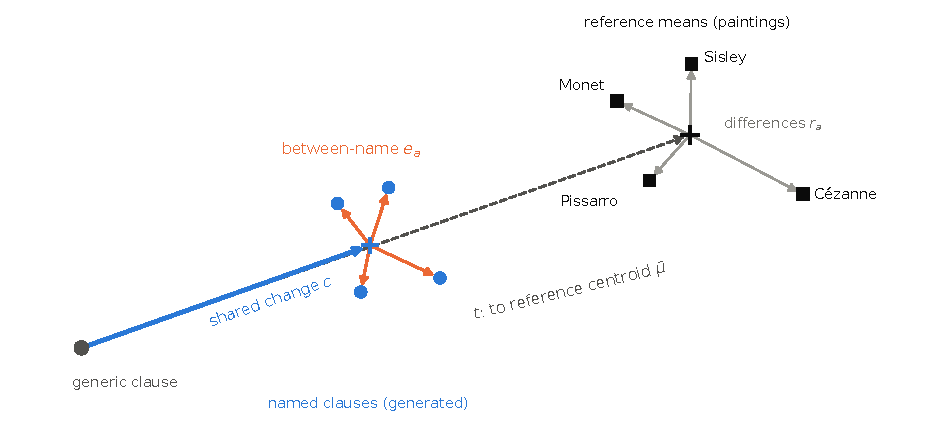
\includegraphics[width=0.92\linewidth]{fig_schematic.pdf}
\caption{분해의 개념도(위치는 설명을 위한 것이며 데이터가 아니다). 일반 지시문을 기준으로, 화가를
지정한 네 출력은 공통 변화 $c$만큼 이동하고 이름 간 차이 $e_a$만큼 서로 다르다. 네 화가의 참조 평균은
그 중심점 $\bar\mu$에서 $r_a$만큼 떨어져 있다. 충실한 모방자라면 일반 출력을 $t$를 따라 끝까지 옮기고
$r_a$를 재현할 것이다. 화가들이 $\|t\|$에 비해 서로 가깝기 때문에, 그 이동의 대부분 역시 공통일 것이다.
그림 속 표기: shared change는 공통 변화, between-name은 이름 간 차이, generic clause는 일반 지시문,
named clauses (generated)는 화가 지정 지시문(생성 이미지), reference means (paintings)는 참조
평균(회화)이다.}
\label{fig:schematic}
\end{figure}

\section{관련 연구}\label{sec:related}

\paragraph{화풍 유사도와 화가 인식.}
\citet{somepalli2024style}은 대조 학습 기반의 화풍 기술자(CSD)를 학습하고, 생성 이미지를 평균 화가
프로토타입에 비추어 점수화한다. \citet{verma2025imitation}은 이러한 화풍 유사도를 이용해 모델이 화가를
모방하기까지 필요한 학습 이미지 수를 추정한다. \citet{casper2023measuring}은 화가 70명에 대한 Stable
Diffusion의 모방 이미지를 CLIP으로 분류하여, 평균적으로 인식 가능함을 보인다. \citet{su2025prompted}은
화가 110명을 대상으로 프롬프트에 지정한 화가를 식별하는 과제를 벤치마크하며, 내용을 통제한 이름 치환과,
같은 시드에서 화가 이름 없이 생성한 이미지와의 비교를 사용한다. \citet{moayeri2025rethinking}은 화가
본인의 작품이 인식 가능하고 그 화풍이 생성 이미지에서도 인식될 때 그 화가의 화풍이 위험에 처한 것으로
보는데, 화가 372명 중 약 5분의 1이 이에 해당한다. \citet{frochte2026csd}은 화가 91명으로 이루어진
말뭉치의 일부에서 원시 CSD 코사인이 같은 화가의 쌍과 다른 화가의 쌍을 구분하지 못함을 보이고, 프롬프트로
생성한 이미지의 인식도 평가한다. \citet{xing2026beyond}은 화가에 기반한 생성이 일반적인 팔레트나
반복되는 모티프 같은 전형적인 지름길에 흔히 의존한다고 관찰한다. 이처럼 화가 미지정 조건과의 비교, 그리고
이름 간 정보를 이용하는 폐쇄 집합 인식은 이미 확립된 지표이다. 우리는 여기에 일반 화풍 대조 조건을
추가하고, 이름이 더하는 변화를 공통 부분과 이름 간 부분으로 나누며, 두 부분 모두를 화가들의 참조
컬렉션에 비추어 벤치마크한다.

\paragraph{화풍의 모방, 보호, 제거.}
Glaze \citep{shan2023glaze}는 미세조정을 통한 모방을 방해하도록 작품에 섭동을 가하며,
\citet{honig2025adversarial}은 사용자 연구를 통해 이러한 보호가 우회될 수 있음을 보인다. 개념
소거(concept erasure) \citep{gandikota2023erasing}와, 화가의 화풍을 일반 회화 같은 앵커 개념으로
사상하는 개념 절제(concept ablation) \citep{kumari2023ablating}는 확산 모델에서 화풍을 제거하며,
UnlearnCanvas \citep{zhang2024unlearncanvas}는 이러한 제거를 벤치마크한다. 개념 절제의 일반 회화 앵커는
우리의 일반 대조 조건과 가깝다.

\paragraph{변화 기반 지표와 미술의 정량적 연구.}
방향성 CLIP 유사도는 이미지 변화의 방향을 텍스트 방향에 비추어 점수화한다
\citep{gal2022stylegannada,brooks2023instructpix2pix}. 이를 화가 이름에 적용하면, 공통 성분을 제거하지
않는 한 그 성분이 포함된다. \citet{deliege2025}은 전문가 평가자와 함께 화풍 모방을 평가하고, AI-Pastiche
\citep{asperti2025pastiche}는 생성 회화의 진정성과 프롬프트 준수를 연구하며, \citet{fu2025aiwikiart}은
작가 귀속과 생성 회화 탐지에서 시각-언어 모델을 시험한다. 정량적 미술 연구는 회화를 색채, 구도, 이미지
통계로 기술하고 \citep{kim2014,sigaki2018,lee2020}, 학습된 임베딩에서 역사적 변화를 추적한다
\citep{kim2026}. 우리의 특징은 이 전통을 따른다. 우리의 추정량은 표상 유사성 분석의 교차검증 거리이며
\citep{diedrichsen2017representational}, 조건부 평가 지표도 이와 비슷하게 조건 내 변동과 조건 평균 간의
관계를 분리한다 \citep{benny2021conditional}.

\section{실험 설계와 측정}\label{sec:design}

\paragraph{화가와 참조 컬렉션.}
참조 컬렉션은 디지털 복제 이미지 649개로 이루어진다. 모네 297개, 시슬레 106개, 피사로 141개, 세잔
105개이다. 포함 기준을 충족한 복제 이미지 가운데 네 개는 측정할 수 없었다(하나는 투명 레이어가 있었고,
셋은 프로파일이 없는 비RGB 색 공간이었다). 포함 기준은 Wikidata에 해당 화가 단독의 회화로 기록되어
있고, 고정된 어휘 목록이 제목과 메타데이터를 야외 장소로 분류하며, Wikimedia Commons에 짧은 변이
1,024픽셀 이상인 복제 이미지가 있는 것이다 \citep{wikimediacommons,vrandecic2014wikidata}. 같은 화가들의
작품 221개로 이루어진 별도의 개발 패널이 특징의 척도를 정한다. 작품은 이 실험 이전에 고정된 해시
규칙으로 두 패널에 배정되었다. 주 비교에는 참조 컬렉션만 사용하고, 개발 패널은 민감도 점검에서 대안
목표로 등장한다. 화가 가운데 셋은 비슷한 모티프를 자주 그린 인상주의 화가이고, 세잔의 작품은 이들과 더
뚜렷이 구별된다. 컬렉션마다 소재의 분포가 다르다(제목 기준으로 모네 작품 297개 중 191개가 수면 장면인
반면 세잔은 105개 중 31개이다. 사람이 확인하지 않은 AI 어시스턴트의 시각적 감사는 작품 870개 중
230개에서 제목 기반 분류와 일치하지 않았다). 이 문제는 내용 대응 목표로 다룬다. 화가 평균에는 항상
동일한 가중치를 준다.

\paragraph{프롬프트.}
고정된 야외 장면 설명 14개가 수면, 건축 환경, 육지, 혼합 구도를 포괄한다(부록 표~\ref{tab:scenes}). 각
장면에 여섯 가지 지시문을 교차한다. 지시문 없음, ``Render as an oil painting.''(유화로 그려라), 그리고
``Render as an oil painting in the style of Claude Monet.''(클로드 모네의 화풍으로 유화를 그려라; 또는
Alfred Sisley, Camille Pissarro, Paul Cezanne. 프롬프트에서는 세잔을 악센트 없이 표기한다)이다. 지시문은
장면 설명 앞에 오며, 모든 프롬프트는 ``No text or frame.''(글자나 액자 없이)로 끝난다.

\paragraph{생성기.}
모든 요청은 OpenRouter 이미지 API를 통해, 구성마다 제공자 하나를 고정하고 대체 경로(fallback)를
비활성화한 상태로 보냈다. \texttt{openai/\allowbreak gpt-\allowbreak image-1}과
\texttt{gpt-\allowbreak image-2}(GPT Image 1과 2), \texttt{gpt-\allowbreak image-\allowbreak
2.5-\allowbreak flare}와 \texttt{gpt-\allowbreak image-\allowbreak 2.5-\allowbreak sunburst}(Flare와
Sunburst)는 모두 중간 품질로, Nano Banana 2(\texttt{google/\allowbreak
gemini-\allowbreak 3.1-\allowbreak flash-\allowbreak image})는 1K 해상도로 요청했고, FLUX.2 Max
(\texttt{black-\allowbreak forest-\allowbreak labs/\allowbreak flux.2-\allowbreak max})도 사용했다. 수집
당시 게이트웨이의 카탈로그는 Flare와 Sunburst를 OpenAI 제공자의 GPT Image 2.5 변형으로 등재하고 있었다.
두 변형이 어떻게 다른지에 대한 추가 문서는 없으며, 계속 제공된다고 보장할 수도 없다. 모든 구성은
$1024\times1024$ 이미지를 반환한다. 구성--장면--지시문 셀마다 별도의 요청을 두 번 보내, 총 1,008개의
이미지를 2026년 9월 10일(UTC)에 수집 전에 고정한 무작위 순서로 수집했다. 응답에는 모델 식별자가 포함되지
않고, 명시적 경로를 유효하지 않은 식별자로 시험하지도 않았으므로, 구성의 이름은 요청한 구성을 가리킨다.
Flare와 Sunburst를 포함해 어느 두 구성의 이미지든, 모든 표현에서 장면--지시문 셀의 91.7\% 이상에서 각
구성 자체의 두 반복 사이보다 서로 더 멀리 떨어져 있다(부록~\ref{app:provenance}).
그림~\ref{fig:examples}는 한 장면을 여섯 지시문 모두로 생성한 예를 보여 준다.

\paragraph{두 화가 집단의 추가.} 공통 비율이 화가들이 서로 얼마나 가까운지에 달려 있는지 검정하기 위해,
위의 결과와 첫 심사 라운드들 이후에 두 집단을 추가했다. 하나는 시대와 화법이 서로 먼 화가들로 이루어진
\term{세기 집단}(century group)으로, 야코프 판 라위스달, 카날레토, 빈센트 반 고흐, 에른스트 루트비히
키르히너이다(17세기부터 20세기까지 세기마다 한 명씩이며, 모두 야외 풍경으로 알려져 있다). 다른 하나는
서로 가까운 허드슨강 화파의 앨버트 비어슈타트, 프레더릭 에드윈 처치, 토머스 콜, 애셔 브라운 듀랜드이다.
이들의 참조 컬렉션은 네 화가 컬렉션과 같은 규칙을 따르되, 이들의 소재에 맞는 제목 용어를 더했고 최소
크기는 두지 않았다. 작품은 788점, 화가당 36--255점이다(부록 표~\ref{tab:v3-panels}). 같은 여섯 구성이
같은 요청 설정으로 같은 14개 장면을 열 가지 지시문(지시 없음, 일반 지시문, 같은 템플릿의 여덟 이름)으로
두 번씩, 2026년 10월 3일에 생성했다. 각 집단은 이 수집에서 얻은 자체의 지시 없음 조건과 일반 지시문
조건으로 분석한다. 31개 특징에서 세기 집단의 참조 화가 산포는 허드슨강 화파의 5.6배이다(부록
표~\ref{tab:v3-predictions}).

\begin{figure}[t]
\centering
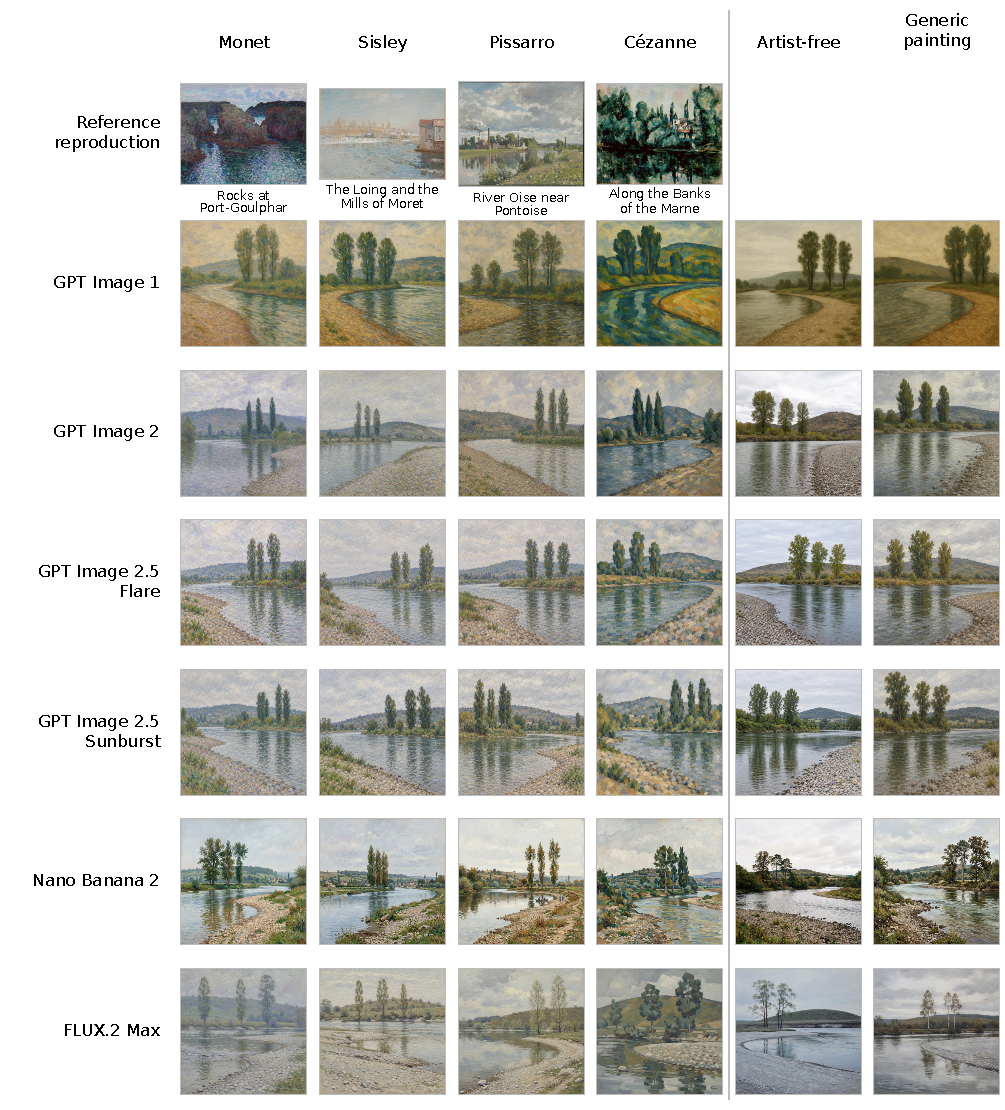
\includegraphics[width=\linewidth]{specificity_original_generated.pdf}
\caption{하나의 장면 설명(자갈 강둑을 지나 굽이치는 강, 건너편 강둑의 나무 세 그루, 흐린 하늘 아래 낮은
언덕)을 각 구성에서 여섯 지시문 모두로 생성한 결과(첫 번째 반복; 결과를 보기 전에 고정한 규칙으로
선정). GPT Image 2.5 Flare와 Sunburst는 본문에서 Flare와 Sunburst로 줄여 쓴다. 맨 위 행은 참고를
위해 화가별로 퍼블릭 도메인 참조 복제 이미지를 하나씩 보여 준다(Wikimedia Commons; 제목은 패널에
표기). 참조 작품은 장면에 맞춰 고른 것이 아니다.}
\label{fig:examples}
\end{figure}

\paragraph{측정.}
주 표현은 세 특징군에 속하는 해석 가능한 좌표 31개로 이루어진다. 색채 특징 11개(명도, 채도, 색상
집중도와 엔트로피, 세 가지 공간 척도에서의 색차), 공간 특징 8개(스펙트럼 기울기와 이방성, 그래디언트
통계, 방향 엔트로피와 균형, 사분면 변동), 텍스처 특징 12개(웨이블릿 에너지, 국소 이진 패턴 엔트로피,
국소 대비)이며, 정의는 부록~\ref{app:features}에 있다. 이미지는 sRGB로 변환하고 짧은 변이 512픽셀이
되도록 크기를 조정한다. 각 좌표는 개발 패널의 화가 가중 중앙값과 사분위 범위로 중심화하고 척도화한다.
또한 모든 이미지를 CLIP ViT-L/14 \citep{radford2021}와 공개된 CSD ViT-L 체크포인트
\citep{somepalli2024style}로 임베딩하며, 각 인코더 고유의 $224\times224$ 중앙 크롭과 단위 정규화된
768차원 출력을 사용한다(부록~\ref{app:learned}). 세 표현은 화가들의 실제 작품을 구분하는 정도가 다르다.
각 개발 작품을 가장 가까운 참조 평균에 배정하면 31개 특징에서 매크로 정확도는 49.8\%이고, 모네 작품의
39.6\%와 시슬레 작품의 30.6\%만 맞게 분류된다. 반면 CLIP에서는 79.8\%, CSD에서는 79.6\%이다. 31개 특징은
해석 가능성 때문에 사전에 지정했고, 임베딩은 이후에 추가했다. 임베딩 지표는 이미지의 내용에 반응할 수
있다 \citep{kynkaanniemi2023role}. CSD는 이 화가들을 화풍 태그에 포함하여 학습되었다.

\section{공통 변화와 이름 간 변화의 분리}\label{sec:method}

아래의 양들은 세 가지 질문에 따라 정리된다. 공통 비율과 그 두 벤치마크
(\ref{sec:split}--\ref{sec:benchmarks}절)는 이름이 더하는 변화 가운데 얼마만큼이 모든 이름에 공통인지를
말해 준다. 정렬 진폭 $\beta$, 상대 크기 $Q$, 정렬 비 $\beta/\sqrt{Q}$, 그리고 1이 화가를 전혀 구분하지
않음을 뜻하는 오차 $D$(\ref{sec:agreement-method}절)는 이름 간 차이가 방향과 크기에서 화가 간 차이와
일치하는지를 말해 준다. 근접도에 대한 정확한 항등식의 공통 항(\ref{sec:proximity}절)은 근접도 이득
가운데 얼마만큼이 모든 이름에 공통인지를 말해 준다. 주요 기호는 부록 표~\ref{tab:estimands}에 정리했다.

\subsection{분해}\label{sec:split}

한 구성에서 장면 $s=1,\dots,S$ ($S=14$), 지시문 $a$, 반복 $k\in\{1,2\}$의 특징 벡터를 $z_{sak}$라 하자.
여기서 $a$는 f(화가 미지정), g(일반), 또는 화가 $1,\dots,4$ 가운데 하나이다. 각 반복 안에서 장면에 대해
평균하면 $\bar z_{ak}$를 얻는다. 일반 지시문을 기준으로, 화가를 지정한 네 평균은 공통 변화와 이름 간
차이로 분해된다.
\begin{equation}
\bar z_{ak}-\bar z_{\mathrm{g}k}=c_k+e_{ak},\qquad
c_k=\tfrac14\sum_{a=1}^4\bar z_{ak}-\bar z_{\mathrm{g}k},\qquad
e_{ak}=\bar z_{ak}-\tfrac14\sum_{a'=1}^4\bar z_{a'k},
\label{eq:split}
\end{equation}
제곱 크기는 다음과 같다.
\begin{equation}
N=4\ip{c_1}{c_2},\qquad B=\sum_{a=1}^4\ip{e_{a1}}{e_{a2}}.
\label{eq:components}
\end{equation}
각 반복이 고정된 평균에, 평균이 0이고 반복 간에 독립인 잡음을 더한 것이라면, 이러한 교차 반복 곱의
기댓값은 평균의 제곱 크기이다. 반면 한 반복을 제곱하면 잡음 분산이 더해진다. 추정값은 음수가 될 수
있으며, 그대로 둔다. \term{공통 비율}은 $N/(N+B)$이다. 이름 간 차이는 기준선에 의존하지 않는다. 화가
미지정 기준선에 대한 분해는 부록~\ref{app:estimators}에 있다.

\subsection{벤치마크}\label{sec:benchmarks}

화가 $a$의 평균 참조 벡터를 $\mu_a$, 그 중심점을 $\bar\mu$, $r_a=\mu_a-\bar\mu$라 하고,
$H=\sum_a\|r_a\|^2$를 \term{참조 화가 산포}라 하자. $B/H$는 생성된 이름 간 차이의 크기를 참조 차이의
크기와 비교한다. 두 벤치마크는 관측된 일반 출력은 그대로 두고 이름의 작용만 바꾼다.
\begin{itemize}
\item \textbf{충실한 모방자.} 화가를 지정한 각 평균이 그 화가의 참조 평균과 같다. 따라서 공통 변화는
$t=\bar\mu-\bar z_{\mathrm{g}}$, 이름 간 차이는 $r_a$가 되고, 공통 비율은 $N^*/(N^*+H)$,
$N^*=4\ip{t_1}{t_2}$이다. 이 값에는 생성 이미지와 촬영된 회화 사이의 거리가 포함되므로, 목표나 한계가
아니라 하나의 기준점이다. 이름 간 차이가 작은 구성은 이 값을 넘을 수 있다.
\item \textbf{정확 차이.} 관측된 공통 변화를 유지하고 이름 간 차이가 $r_a$와 같다고 하면 $N/(N+H)$를
얻는다. 이렇게 하면 일반 출력이 회화에서 얼마나 떨어져 있는지에 대한 의존성이 사라진다. 관측된 비율은
$B/H$가 1과 다른 만큼만 이 값과 달라진다.
\end{itemize}
관측된 비율은 서로 다른 두 가지 양을 통해 충실한 모방자의 비율과 달라진다. 공통 변화가 $t$의 얼마만큼을
덮는지, 그리고 이름 간 차이가 $H$에 비해 얼마나 큰지이다. 우리는 교차 반복 곱으로 보정한 $c$와 $t$ 사이의
코사인과, $t$ 방향으로 덮인 거리의 비율 $\lambda=\ip{c}{t}/\|t\|^2$를 보고한다.

\subsection{참조 차이와의 일치}\label{sec:agreement-method}

이름 간 차이가 참조 차이와 일치하는지 검정하기 위해, 각 장면을 따로 중심화하여
$d_{sak}=z_{sak}-\frac14\sum_{a'}z_{sa'k}$로 두고 다음을 정의한다.
\begin{equation}
\widehat\beta=\frac1S\sum_s\frac{1}{2}\sum_{k=1}^2\frac{\sum_a\ip{d_{sak}}{r_a}}{H},\qquad
\widehat D=\frac1S\sum_s\frac1H\sum_a\ip{d_{sa1}-r_a}{d_{sa2}-r_a};
\label{eq:beta-d}
\end{equation}
이하에서는 모자 기호를 생략한다. 정렬 진폭 $\beta$는 생성된 차이를 참조 패턴에 사영한 것이다.
$\beta=1$이면 그 패턴 방향의 크기가 참조와 일치하고, $\beta>0$이면 전체적으로 올바른 방향의 반응임을
뜻한다. 오차 $D$는 다른 방향의 차이까지 센다. 그 기댓값은 완전히 일치할 때 0, 이름이 아무런 차이도
만들지 않을 때 1, 참조 패턴이 $\kappa$배 크기로 재현될 때 $(\kappa-1)^2$이다. 참조에 대한 생성 차이의
제곱 크기 $Q=(SH)^{-1}\sum_{s,a}\ip{d_{sa1}}{d_{sa2}}$를 쓰면 $D=1-2\beta+Q$이다. 사전 지정한 분해는
$D$를 참조 패턴 방향 진폭의 오차와, 그 패턴에 직교하는 차이의 크기인 패턴 외 부분의 합으로 정확히
나타낸다(부록~\ref{app:estimators}). 정렬 비 $\beta/\sqrt{Q}$는 장면별 차이가 통합 참조 패턴과 얼마나
정렬되는지를 나타낸다. 차이의 크기를 재조정해도 변하지 않지만, 패턴 외 차이와 장면 간 변동이 있으면
낮아진다. 차이를 최적으로 재조정하면 $D=1-\beta^2/Q$가 남는다. $D_{\mathrm{held}}$는 다른 장면들에서
적합한 재조정을 적용한 것이므로 정렬 비를 거의 그대로 따른다. 모든 장면을 동일한 통합 목표와 비교하므로
$D$는 장면마다 달라지는 차이에도 벌점을 준다. 즉 $D=D_{\mathrm{agg}}+V_{\mathrm{scene}}$이며, 여기서
$D_{\mathrm{agg}}$는 장면 평균 차이를 평가하고 $Q=B/H+V_{\mathrm{scene}}$이다. 장면 평균 정렬은
$\beta/\sqrt{B/H}$이다. 화가당 두 작품이 한 장면의 두 반복을 대신하게 하면 실제 회화도 $D=0$에 이르지
못하므로, 홀드아웃한 참조 회화에 대해서도 이 오차를 보고한다. 여기서 특이성은 주어진 표현에서 화가들의
참조 평균 간 차이와 일치하는 정도를 뜻하며, 지각적 판단은 들어가지 않는다.

\subsection{임베딩에서의 근접도와 인식}\label{sec:proximity}

임베딩에서 화가 $a$와 일반 지시문에 대한 평균 단위 임베딩을 $g_a$와 $g_{\mathrm{g}}$, 그 화가의 단위 참조
임베딩의 평균을 $\mu_a$라 하자. 그러면 $g_a^\top\mu_a$는 화가 지정 이미지와 그 화가의 참조 작품 사이의
평균 코사인 유사도이다. 이 유사도에서 화가 지정 조건이 일반 조건보다 얻는 이득은 다음과 같이 정확히
분해된다.
\begin{equation}
\underbrace{\frac14\sum_a g_a^\top\mu_a-g_{\mathrm{g}}^\top\bar\mu}_{\text{근접도 이득}}
=\underbrace{(\bar g-g_{\mathrm{g}})^\top\bar\mu}_{\text{공통}}
+\underbrace{\frac{H\beta}{4}}_{\text{화가 특이적}},
\label{eq:prototype-gain}
\end{equation}
여기서 $H$와 $\beta$는 해당 임베딩에서 계산한다(부록~\ref{app:learned}). 화가가 $K$명이면 화가 특이적
항은 $H\beta/K$이다. 공통 항은 어떤 이름이 어떤 이미지를 만들었는지에 의존하지 않는다. 이 항등식은 이미지
임베딩에 대해 선형인 모든 점수에 성립하며, 단위 길이로 정규화한 프로토타입과의 코사인 유사도도 여기에
포함된다. 정규화한 프로토타입을 쓰면 아래의 비율은 최대 0.5포인트 달라진다(부록
표~\ref{tab:learned-settings}). 검색, 상위 $k$개 유사도, 모방 판정처럼 순위·최댓값·임계값에 기반한
지표는 이 항등식의 범위 밖이다. 기준선이 없는 원시 근접도에는 $g_{\mathrm{g}}^\top\bar\mu$가 더해지는데,
이 역시 이름에 의존하지 않는다. 충실한 모방자 벤치마크는 $g_a=\mu_a$로 두고, 정확 차이 벤치마크는 공통
항을 유지한 채 화가 특이적 항을 $H/4$로 둔다. 따라서 공통 항이 $H/4$를 넘으면, 곧 화가들의 공통
프로토타입을 향한 공통 이동이 화가 산포의 4분의 1보다 크면, 정확 차이 생성기의 이득에서 공통 항이 과반을
차지한다. 인식은 별개의 지표이다. 화가를 지정한 각 이미지를 단위 길이로 정규화한 참조 프로토타입 가운데
코사인 유사도가 가장 큰 것에 배정하고, 네 화가에 대한 매크로 정확도를 보고한다.

\subsection{추론과 분석의 지위}\label{sec:inference}

수집 전에 프로토콜은 31개 특징에서 21개 비교로 이루어진 추론 검정군, 곧 여섯 정렬 진폭과 $D$의 쌍별 차이
15개를 고정하고, 장면 대응(paired-scene) 스튜던트 구간과 21개 전체에 대한 본페로니 보정을 지정했다.
프로토콜은 또한 쌍별 차이에 대한 미보정 구간과 장면 대응 부트스트랩(부록 표~\ref{tab:pairs}), 화가
내에서의 참조 작품 재표집, 화가 미지정 기준의 공통/이름 간 분해, 참조 패턴 방향과 패턴 외로의 $D$ 분해,
분포 진단(부록 표~\ref{tab:diversity})을 규정했다. 프로토콜의 장면 고정효과 회귀는 쌍별 차이를 그대로
재현하며, 전체 분포를 보여 주는 참조 PCA 도식은 평균의 사영도(부록 그림~\ref{fig:projection})로
대신했다. 그 밖의 구간은 모두 미보정이다. 장면별 통계량에는 장면 대응 스튜던트 구간을, 재표집한
통계량에는 백분위수 구간을 쓴다. 구간이 비교값을 포함하지 않을 때 그 차이가 \term{판별된다}(resolved)고
한다. 보정된 구간은 사전 지정한 21개 비교에만 쓰이며, $D$와 1의 비교는 이 검정군에 속하지 않는다.
프로토콜은 $D$만으로 구성의 순위를 매겼다. 정렬 비와 $D_{\mathrm{held}}$, 그리고 이들의 재표집은 $D$
순위가 표현에 따라 달라진다는 사실을 알게 된 뒤, 수집 이후에 정의했다. 구간은 직접 작성한 14개 장면과
유한한 참조 패널에 대한 것이며, 새로운 장면이나 화가에 대한 것이 아니다. 첫 번째 수집 시도는 게이트웨이
경로가 유효하지 않은 모델 식별자를 받아들이는 것이 확인되어 어떤 이미지도 측정하기 전에 중단했고, 이후
예산에 맞추기 위해 장면 패널을 16개에서 14개로 줄였다(부록~\ref{app:provenance}). 그 밖의 모든 것, 곧
일반 기준선 분해, 벤치마크, 임베딩 분석, 인식, 실제 회화 대조군, 그리고 이 양들의 재표집은, 다른 결과가
이미 알려진 이미지에 대해 서면 계획에 따라 사후에 추가했다. 보충 자료에 포함된 이 계획서들은 각 계획을
작성할 당시 이미 알려져 있던 값을 기록하고 있다. 이 분석들은 서술적이다.

두 번째 수집은 그 이미지가 생기기 전에 작성한 자체 프로토콜을 따랐다. 이 프로토콜은 31개 특징에서 두
검정을 정했고, CLIP과 CSD의 같은 통계량은 보조로 두었다. H1은 구성에 걸쳐 평균한 세기 집단의 공통
비율이 허드슨강 화파보다 낮다는 것이며, 짝지은 장면 재표집 5,000회에서 95\% 구간을 구한다. H2는 새
여덟 화가의 쌍 28개에 걸쳐, 두 이름의 이미지 간 교차 반복 거리가 화가들의 참조 평균 간 거리와 함께
커진다는 것이며, 구성에 걸쳐 평균한 스피어만 상관으로 측정하고 화가 이름표의 재배열 40,320가지 전부에
대해 정확 검정한다. 참조 거리는 패널 크기에 대해 보정한다. 프로토콜은 예측된 참조 산포와 충실한 모방자
벤치마크도 기록했고, 이 논문의 추정량을 각 집단에 적용했다. 임베딩 지표(구간, 인식, 근접도)에 대한 별도
계획은 이미지를 측정하기 전에 확정했다. 참조 규칙에 대한 두 번의 수정은 어떤 요청보다도 앞섰고, 게이트웨이
오류에 대해 유보된 금액을 흡수하기 위해 수집 중에 지출 상한을 올렸다(부록~\ref{app:second}).

\section{결과}\label{sec:results}

첫 번째 수집의 이미지 1,008개 모두에서 유효한 측정값을 얻었다. 두 번째 수집에서는 요청 1,680건 가운데
1,678건이 이미지를 반환했다. 한 제공자의 안전 시스템이 두 건(듀랜드를 지정한 Sunburst와 비어슈타트를
지정한 GPT Image 1, 서로 다른 두 장면)을 거부했으며, 이는 대체하지 않으므로 집단 간 검정은 모든 조건과
구성이 갖추어진 12개 장면을 사용한다. 범위, 차이, 비율은 반올림하지 않은 값으로 계산했다.

\subsection{이름이 더하는 변화의 대부분은 공통이며, 충실한 모방이라면 공통 비율이 더 높을 것이다}\label{sec:shared}

% 한국어판: paper/tmlr_ko/build_korean.py 가 생성한다. 직접 고치지 않는다.
% Generated by paper/tmlr/build_assets.py; do not edit by hand.
% input reports/painter_tmlr_diagnostics_v1/analysis.json sha256 76792fa35f90e3d8fec1a75b0eec27d69cac14ed875fce8b64096b8e2525a4d4
% input reports/painter_tmlr_diagnostics_v2/analysis.json sha256 bed891f767a98f4b281b6783b1021956f4d2c3ff80becbf6b2693ee45987ef1a
\begin{table}[t]
\caption{일반 지시문에 더해 네 이름이 추가하는 변화의 공통 비율 $N/(N+B)$(31개 특징)과 장면 재표집 5,000회에서 구한 95\% 구간, 그리고 참조 화가 산포 $H$에 대한 공통 변화($N$)와 이름 간 차이($B$)의 제곱 크기. 충실: 같은 일반 출력에서 출발하여 화가를 지정한 각 평균이 그 화가의 참조 평균과 같을 때의 비율. 정확 차이: 관측된 공통 변화를 유지하고 $B/H$가 1일 때의 비율, $N/(N+H)$. 관측$<$충실: 관측 비율이 충실한 모방자의 비율보다 낮은 장면 재표집의 비율. 공통 변화의 방향은 부록 표~\ref{tab:direction}에 있다.}
\label{tab:shared}
\vspace{2pt}
\centering\small\setlength{\tabcolsep}{4pt}
\begin{tabular}{@{}lrcrrrrr@{}}
\toprule
 & \multicolumn{4}{c}{관측} & \multicolumn{3}{c}{벤치마크}\\
\cmidrule(lr){2-5}\cmidrule(l){6-8}
구성 & 비율 (\%) & 장면 95\% & $N/H$ & $B/H$ & 충실 (\%) & 정확 차이 (\%) & 관측$<$충실 (\%)\\
\midrule
GPT Image 1 & 71.3 & [67.6, 74.9] & 5.26 & 2.12 & 95.2 & 84.0 & 100.0\\
GPT Image 2 & 70.9 & [66.5, 75.6] & 4.98 & 2.04 & 89.3 & 83.3 & 100.0\\
Flare & 71.1 & [66.7, 76.7] & 4.99 & 2.03 & 84.8 & 83.3 & 100.0\\
Sunburst & 66.7 & [63.3, 71.1] & 3.97 & 1.98 & 86.9 & 79.9 & 100.0\\
Nano Banana 2 & 69.1 & [52.0, 75.8] & 1.36 & 0.61 & 92.5 & 57.6 & 100.0\\
FLUX.2 Max & 88.4 & [76.8, 94.2] & 5.34 & 0.70 & 90.4 & 84.2 & 84.1\\
\bottomrule
\end{tabular}
\end{table}


일반 지시문에 더해 이름이 추가하는 제곱 변화량의 66.7--88.4\%는 네 이름 모두에 공통이다
(표~\ref{tab:shared}). 같은 일반 출력에서 출발하는 충실한 모방자라면 84.8--95.2\%를 보일 것이다
(그림~\ref{fig:benchmark}). 일반 출력은 네 화가가 서로 떨어져 있는 것보다 회화에서 훨씬 더 멀리 있으므로,
회화를 향한 충실한 이동은 대부분 공통이기 때문이다. 다섯 구성에서는 모든 장면 재표집에서 관측 비율이
충실한 모방자의 비율보다 낮다. FLUX.2 Max는 재표집의 84.1\%에서 낮으며, 그 구간 [76.8, 94.2]는 충실한
모방자의 값을 포함한다.

정확 차이 벤치마크는 회화까지의 거리를 비교에서 제거한다. 각 구성의 공통 변화를 유지하면서 화가 간
차이를 정확히 재현하는 생성기는 57.6--84.2\%를 보일 것이므로, 이름 간 차이가 완벽하더라도 모든 구성에서
변화의 대부분은 공통으로 남는다. 관측 비율은 이름 간 차이의 크기를 통해서만 이 벤치마크와 달라진다.
$B/H$는 네 GPT 구성에서 1.98--2.12여서 이들의 비율은 벤치마크보다 낮고, Nano Banana 2와 FLUX.2
Max에서는 0.61--0.70이어서 벤치마크보다 높다. 그러므로 충실한 모방자의 값보다 낮다고 해서 더
특이적이라는 뜻은 아니다. 예를 들어 Nano Banana 2가 충실한 모방자의 값보다 훨씬 낮은 것은 공통 변화가
참조 중심점까지 거리의 24.8\%만 덮기 때문이다. 화가 간 차이가 정확하다면 그 비율은 57.6\%로 떨어질
것이다.

공통 변화는 참조 중심점을 향하며, 보정된 코사인은 0.57--0.86이다(부록 표~\ref{tab:direction}). Nano
Banana 2와 FLUX.2 Max에서는 공통 변화 제곱 크기의 55.5\%와 52.8\%가 화가 미지정에서 일반 조건으로의 이동
방향에도 놓여 있는 반면, 네 GPT 구성에서는 0.1--22.0\%이다. 즉 이 두 구성에서는 이름이 더하는 변화의
일부가 일반 회화 지시의 연장이다. 장면 내에서 계산하면 공통 비율은 52.8--93.6\%이고, 회화 지시 자체를
포함하는 화가 미지정 기준선에 대해서는 82.5--95.7\%이다(부록~\ref{app:hand}).

\begin{figure}[t]
\centering
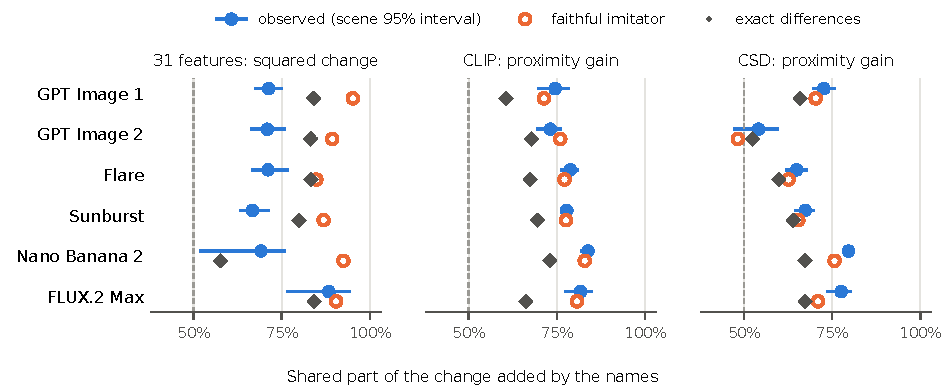
\includegraphics[width=\linewidth]{fig_benchmark.pdf}
\caption{일반 지시문에 더해 네 이름이 추가하는 변화 가운데 공통인 부분(채운 점; 장면 재표집의 95\%
구간 포함)과, 충실한 모방자(빈 원) 및 정확 차이 생성기(마름모)가 보일 값. 왼쪽: 31개 특징에서의 제곱
변화량. 가운데와 오른쪽: 임베딩에서 근접도 이득 가운데 공통 항의 비율(식~\ref{eq:prototype-gain}). 제곱
변화량은 참조 패턴에서 벗어난 것까지 포함해 이름 간 차이 전체를 세는 반면, 근접도 이득은 그 가운데
정렬된 부분 $H\beta/4$만 센다. 관측값이 왼쪽에서는 충실한 모방자의 값보다 낮지만 임베딩에서는 대체로 그
이상인 것은 이 때문이다(임베딩에서의 제곱 변화량 비율은 부록 표~\ref{tab:learned-squared} 참조).
임베딩에서는 충실한 모방자 벤치마크가 참조 작품의 다양성도 물려받는다. 참조 작품의 평균 임베딩은 생성
이미지의 평균 임베딩보다 짧으며, CSD에서 특히 그렇다. 점선은 50\%를 나타낸다. 그림 속 표기: observed는
관측값, faithful imitator는 충실한 모방자, exact differences는 정확 차이, squared change는 제곱
변화량, proximity gain은 근접도 이득이다.}
\label{fig:benchmark}
\end{figure}

\subsection{공통 비율은 화가들이 서로 얼마나 가까운지를 따른다}\label{sec:groups}

% 한국어판: paper/tmlr_ko/build_korean.py 가 생성한다. 직접 고치지 않는다.
% Generated by paper/tmlr/build_assets.py; do not edit by hand.
% input reports/painter_tmlr_diagnostics_v2/analysis.json sha256 bed891f767a98f4b281b6783b1021956f4d2c3ff80becbf6b2693ee45987ef1a
% input reports/painter_specificity_v3/analysis.json sha256 75ef2a23c04a5c570fd224a0ada396271ad7026ef0657a1908023daca709cbc4
\begin{table}[t]
\caption{일반 지시문에 더해 네 이름이 추가하는 변화의 공통 비율 $N/(N+B)$ (\%), 관측값과 충실한 모방자의 값, 31개 특징, 네 인상파 화가(첫 번째 수집)와 추가한 두 집단(두 번째 수집, 각자의 일반 지시문 조건). 마지막 열: 세기 집단의 비율에서 허드슨강 화파의 비율을 뺀 값과, 짝지은 장면 재표집 5,000회에서 구한 본페로니 보정(여섯 구성) 백분위 구간. 평균 행은 사전 지정 검정 H1이며 95\% 구간을 함께 적었다.}
\label{tab:v3-shared}
\vspace{2pt}
\centering\small\setlength{\tabcolsep}{3.5pt}
\begin{tabular}{@{}lrrrrrrrc@{}}
\toprule
 & \multicolumn{2}{c}{인상파} & \multicolumn{2}{c}{세기 집단} & \multicolumn{2}{c}{허드슨강 화파} & \multicolumn{2}{c}{세기 $-$ 허드슨}\\
\cmidrule(lr){2-3}\cmidrule(lr){4-5}\cmidrule(lr){6-7}\cmidrule(l){8-9}
구성 & 관측 & 충실 & 관측 & 충실 & 관측 & 충실 & 차이 & 95\%\\
\midrule
GPT Image 1 & 71.3 & 95.2 & 29.5 & 67.6 & 95.7 & 90.2 & $-$66.1 & [$-$76.8, $-$53.3]\\
GPT Image 2 & 70.9 & 89.3 & 18.5 & 53.3 & 98.6 & 92.5 & $-$80.1 & [$-$84.3, $-$69.2]\\
Flare & 71.1 & 84.8 & 18.9 & 66.8 & 93.8 & 96.0 & $-$75.0 & [$-$78.8, $-$65.0]\\
Sunburst & 66.7 & 86.9 & 23.6 & 67.8 & 93.5 & 96.2 & $-$69.9 & [$-$75.0, $-$64.4]\\
Nano Banana 2 & 69.1 & 92.5 & 21.6 & 75.4 & 95.1 & 97.0 & $-$73.5 & [$-$80.1, $-$59.7]\\
FLUX.2 Max & 88.4 & 90.4 & 17.7 & 45.0 & 89.4 & 89.4 & $-$71.6 & [$-$198.2, +90.2]\\
\midrule
평균 & & & & & & & $-$72.7 & [$-$76.5, $-$62.6]\\
\bottomrule
\end{tabular}
\end{table}


두 번째 수집의 사전 지정 검정은 둘 다 지지된다(표~\ref{tab:v3-shared}). 31개 특징에서 세기 집단의
공통 비율은 17.7--29.5\%, 허드슨강 화파는 89.4--98.6\%이다. 구성에 걸쳐 평균하면 세기 집단이
72.7퍼센트포인트 낮고, CLIP에서는 40.1, CSD에서는 47.4퍼센트포인트 낮다(부록 표~\ref{tab:v3-tests}).
수집 전에 기록한 예측은 이 순서를 예상했다. 새 일반 출력에서 출발하면 충실한 모방자는 세기 집단에서
45.0--75.4\%, 허드슨강 화파에서 89.4--97.0\%를 보일 것이다. 여덟 화가의 쌍 28개에 걸쳐, 두 이름의
이미지 간 거리는 화가들의 참조 평균 간 거리와 함께 커지며(그림~\ref{fig:v3-pairs}), 스피어만 상관은
31개 특징에서 0.85, CLIP에서 0.86, CSD에서 0.92이다.

\begin{figure}[t]
\centering
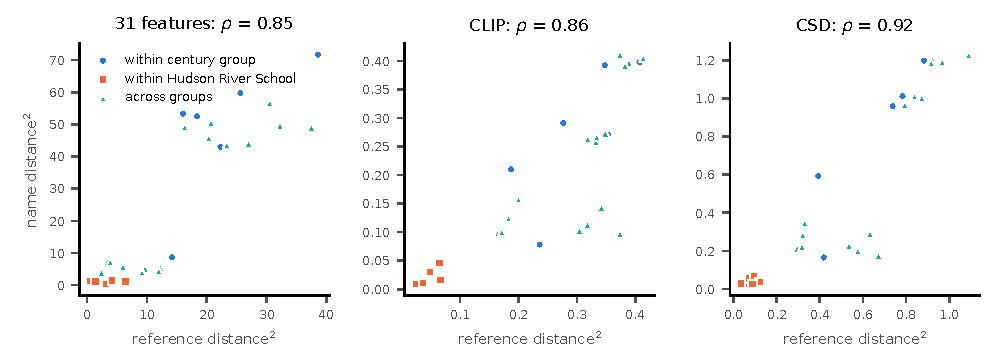
\includegraphics[width=\linewidth]{fig_v3_pairs.pdf}
\caption{두 번째 수집의 여덟 화가로 이루어진 쌍 28개 각각에 대해, 두 이름의 이미지 간 제곱 거리(장면
평균, 서로 다른 반복 간의 곱, 구성 평균)를 화가들의 참조 평균 간 제곱 거리(패널 크기에 대해 보정)에 대해
표현별로 나타냈다. 세기 집단 안의 쌍(원), 허드슨강 화파 안의 쌍(사각형), 두 집단에 걸친 쌍(삼각형).
그림 속 표기: within century group은 세기 집단 안, within Hudson River School은 허드슨강 화파 안, across
groups는 집단 간, name distance는 이름 간 거리, reference distance는 참조 거리.}
\label{fig:v3-pairs}
\end{figure}

두 집단은 이름이 공통 변화 외에 하는 일에서 다르다. 세기 집단에서는 이름 간 차이가 참조 차이와 방향이
맞고 크기도 대략 맞는다. 31개 특징에서 $\beta$는 0.840--1.292이고 정렬 비는 0.698--0.805로 인상파
화가들에 대한 어떤 구성보다도 높으며, 임베딩에서 프롬프트에 지정한 화가는 이미지의 71.9--89.6\%에서
인식된다(네 화가 중 선택, 우연 수준 25\%). 허드슨강 화파에서는 이름들이 거의 다르지 않다. $\beta$는
특징에서 $-$0.014에서 0.198, 임베딩에서 0.095--0.395이고, 인식률은 29.2--50.0\%이며, GPT Image 1과
GPT Image 2에서는 공통 비율이 충실한 모방자 벤치마크보다도 높다(부록 표~\ref{tab:v3-detail}과
\ref{tab:v3-embeddings}). 작은 패널로는 이를 설명할 수 없다. 허드슨강 화파의 산포를 패널 크기에 대해
보정하면 6.24에서 4.21로 낮아지므로, 보정된 평균을 모방하는 생성기도 관측된 패턴에 대해 $\beta$가 0.68
근처일 것이다. 인상파 화가들은 두 집단 사이에 놓인다. 근접도도 이를 따른다. 식~\ref{eq:prototype-gain}의
공통 항은 허드슨강 화파에서 임베딩 근접도 이득의 92.5--98.3\%를, 세기 집단에서는 6.5--49.0\%를
차지한다. 두 수집에서 세 주 간격으로 똑같이 요청한 지시 없음 및 일반 지시문 출력은 반복 잡음 이상으로
다르지 않다(부록 표~\ref{tab:v3-drift}).

\subsection{서로 가까운 화가들에서는 근접도 이득이 주로 공통 변화를 측정한다}\label{sec:learned}

% 한국어판: paper/tmlr_ko/build_korean.py 가 생성한다. 직접 고치지 않는다.
% Generated by paper/tmlr/build_assets.py; do not edit by hand.
% input reports/painter_tmlr_diagnostics_v2/analysis.json sha256 bed891f767a98f4b281b6783b1021956f4d2c3ff80becbf6b2693ee45987ef1a
\begin{table}[t]
\caption{CLIP과 CSD에서 화가 지정 조건이 일반 조건보다 얻는 근접도 이득 가운데 공통 부분의 비율(\%)(식~\ref{eq:prototype-gain})과 장면 재표집 5,000회에서 구한 95\% 구간. 충실: 화가를 지정한 모든 평균 임베딩이 그 화가의 평균 참조 임베딩과 같을 때의 같은 비율. 정확 차이: 관측된 공통 항을 유지하고 화가 특이적 항이 참조 값 $H/4$일 때의 비율.}
\label{tab:learned}
\vspace{2pt}
\centering\small\setlength{\tabcolsep}{3.5pt}
\begin{tabular}{@{}lrcrrrcrr@{}}
\toprule
 & \multicolumn{4}{c}{CLIP} & \multicolumn{4}{c}{CSD}\\
\cmidrule(lr){2-5}\cmidrule(l){6-9}
구성 & 관측 & 장면 95\% & 충실 & 정확 차이 & 관측 & 장면 95\% & 충실 & 정확 차이\\
\midrule
GPT Image 1 & 74.5 & [69.9, 78.2] & 71.3 & 60.6 & 72.7 & [69.7, 75.6] & 70.4 & 66.0\\
GPT Image 2 & 73.2 & [69.7, 75.9] & 76.0 & 67.7 & 54.2 & [47.4, 59.3] & 48.3 & 52.5\\
Flare & 78.8 & [76.4, 80.7] & 77.1 & 67.5 & 65.0 & [62.1, 67.6] & 62.7 & 59.9\\
Sunburst & 77.7 & [76.3, 79.2] & 77.6 & 69.4 & 67.4 & [64.6, 69.6] & 65.4 & 64.0\\
Nano Banana 2 & 83.8 & [82.0, 85.3] & 82.9 & 73.0 & 79.7 & [78.5, 80.8] & 75.7 & 67.3\\
FLUX.2 Max & 81.7 & [77.4, 84.9] & 80.7 & 66.2 & 77.6 & [73.7, 80.3] & 71.0 & 67.4\\
\bottomrule
\end{tabular}
\end{table}

% 한국어판: paper/tmlr_ko/build_korean.py 가 생성한다. 직접 고치지 않는다.
% Generated by paper/tmlr/build_assets.py; do not edit by hand.
% input reports/painter_learned_audit_v1/analysis.json sha256 06c77de4be133afc203dda122b2816d4f866e1389999f18bc94b3d9c668f28f7
% input reports/painter_tmlr_diagnostics_v5/analysis.json sha256 5747902e4fae5ff111a52b5f2b8da112bc26c611555e82314b278de953981f6b
\begin{table}[t]
\caption{각 임베딩에서 같은 이미지에 대한 지표. 근접도: 프롬프트에 지정한 화가의 참조 작품과의 평균 코사인 유사도에서 화가 지정 조건이 일반 조건보다 얻는 이득으로, 식~\ref{eq:prototype-gain}에 따라 공통 항과 화가 특이적 항 $H\beta/4$로 나뉜다. 인식: 화가 지정 이미지 112개 각각을 가장 가까운 참조 프로토타입으로 프롬프트의 화가에 배정할 때의 매크로 정확도(우연 수준 25\%). 일치: 정렬 비(높을수록 좋음)와 오차 $D$(낮을수록 좋음). 31개 특징의 값은 표~\ref{tab:agreement}에 있다. 굵은 글씨는 각 열과 임베딩에서 가장 큰 값($D$는 가장 낮은 값)을 나타낸다. 장면 재표집에서 각 구성이 얼마나 자주 가장 좋은지는 부록 표~\ref{tab:stability}에 있다.}
\label{tab:readouts}
\vspace{2pt}
\centering\small
\begin{tabular}{@{}lrrrrrr@{}}
\toprule
 & \multicolumn{3}{c}{근접도 이득} & 인식 & \multicolumn{2}{c}{일치}\\
\cmidrule(lr){2-4}\cmidrule(l){6-7}
구성 & 전체 & 공통 & 화가 특이적 & (\%) & $\beta/\sqrt{Q}$ & $D$\\
\midrule
\multicolumn{7}{@{}l}{\textit{CLIP}}\\
GPT Image 1 & 0.072 & 0.053 & 0.018 & 60.7 & 0.555 & \textbf{0.847}\\
GPT Image 2 & 0.100 & 0.073 & \textbf{0.027} & \textbf{68.8} & \textbf{0.609} & 1.061\\
Flare & 0.091 & 0.072 & 0.019 & 59.8 & 0.515 & 1.057\\
Sunburst & 0.101 & 0.079 & 0.023 & 58.9 & 0.543 & 1.136\\
Nano Banana 2 & \textbf{0.112} & 0.094 & 0.018 & 51.8 & 0.493 & 1.078\\
FLUX.2 Max & 0.083 & 0.068 & 0.015 & 41.1 & 0.453 & 1.058\\
\midrule
\multicolumn{7}{@{}l}{\textit{CSD}}\\
GPT Image 1 & \textbf{0.217} & 0.158 & 0.059 & 72.3 & 0.667 & 0.735\\
GPT Image 2 & 0.166 & 0.090 & \textbf{0.076} & \textbf{75.9} & \textbf{0.737} & 0.741\\
Flare & 0.187 & 0.121 & 0.065 & 62.5 & 0.673 & 0.819\\
Sunburst & 0.214 & 0.144 & 0.070 & 61.6 & 0.666 & 0.944\\
Nano Banana 2 & 0.210 & 0.167 & 0.043 & 50.9 & 0.513 & 0.999\\
FLUX.2 Max & \textbf{0.217} & 0.168 & 0.049 & 39.3 & 0.627 & \textbf{0.714}\\
\bottomrule
\end{tabular}
\end{table}


CLIP과 CSD에서 식~\ref{eq:prototype-gain}의 공통 항은 화가 지정 조건이 일반 조건보다 얻는 근접도 이득의
73.2--83.8\%와 54.2--79.7\%를 차지한다(표~\ref{tab:learned}). 충실한 모방자라면 이득의 71.3--82.9\%와
48.3--75.7\%를 같은 항에서 얻을 것이다. 관측된 비율은 이 값들과 $-$2.8에서 +6.5퍼센트포인트만큼 차이
나며, CSD에서는 여섯 구성 모두에서 이 값보다 높다. 화가 간 차이가 정확한 경우에도 공통 항은 이득의
60.6--73.0\%(CLIP)와 52.5--67.4\%(CSD)를 차지할 것이다. 네 화가의 공통 프로토타입을 향한 공통 이동이 모든
경우에 화가 산포의 4분의 1을 넘기 때문이다. 구성--인코더 쌍 12개 중 11개에서 공통 항은 이득의 과반이며
장면 구간도 50\% 위에 있다. 예외는 CSD에서의 GPT Image 2로, 54.2\% [47.4, 59.3]이며 충실한 모방자라면
48.3\%를 얻을 것이다. 화가별로 보면 12개 쌍 중 11개에서 세잔의 이득이 가장 덜 공통적이며, 34.6\%까지
낮아진다(부록 표~\ref{tab:per-painter}). 감사한 원본 영역이나 개발 패널을 참조 목표로 사용해도 관측
비율은 최대 1.6포인트 달라질 뿐이다(부록 표~\ref{tab:learned-settings}).

공통 항은 구성 간 이득의 차이도 좌우하는데, 근접도는 바로 이런 방식으로 모델을 비교하는 데 쓰인다
(표~\ref{tab:readouts}). 여섯 구성에 걸쳐 이득과 공통 항의 상관계수는 CLIP에서 0.96 [0.91, 0.98],
CSD에서 0.95 [0.79, 0.99]이다(장면 재표집의 95\% 구간). 구성 간 변동도 공통 항이 화가 특이적 항보다
커서, 분산 기준으로 CLIP에서 11배 [4.6, 29.3], CSD에서 5.8배 [2.5, 13.8]이다. 구성이 여섯 개뿐이고
이득이 두 항의 합이므로, 이 수치들은 서술적이다. CLIP에서는 이득에 따른 구성의 순위가 공통 항에 따른
순위와 정확히 같고, CSD에서는 이득과 화가 특이적 항의 상관계수가 $-$0.65이다. Nano Banana 2는 CLIP
이득이 가장 크지만 화가 특이적 항은 다섯 번째로 크고, GPT Image 2는 CSD 이득이 가장 작지만 화가 특이적
항은 가장 크다.

\subsection{이름 간 차이는 올바른 방향을 가리키지만, 크기는 제각각이다}\label{sec:agreement}

% 한국어판: paper/tmlr_ko/build_korean.py 가 생성한다. 직접 고치지 않는다.
% Generated by paper/tmlr/build_assets.py; do not edit by hand.
% input reports/painter_specificity_v2/psv2-20260911/models.csv sha256 eed121f77626d8a37235b5bb19e370e3fbd7b6bae44b559d1b866e27e9cac41c
% input reports/painter_specificity_review_v1/analysis.json sha256 2fabb78e15dfcc7b027a73170f6ad0c87af0196c754b4e6f45275269c2c961e2
% input data/manifests/painter_specificity_v2/psv2-20260911/analysis.json sha256 c1d21b16f840a10fd253c1d558743a09671acf3d4e48601ddcc96625a5a90be0
% input reports/painter_tmlr_diagnostics_v2/analysis.json sha256 bed891f767a98f4b281b6783b1021956f4d2c3ff80becbf6b2693ee45987ef1a
\begin{table}[t]
\caption{이름 간 차이와 참조 화가 간 차이의 일치(31개 특징). $\beta=1$이면 참조 패턴 방향의 크기가 참조와 일치한다. $Q$는 참조에 대한 생성 차이의 제곱 크기이고, $\beta/\sqrt{Q}$는 참조 패턴과의 정렬로서 차이의 크기를 재조정해도 변하지 않는다(참조 패턴을 일정 배율로 복제한 경우 1). $D=1-2\beta+Q$는 완전히 일치할 때 0, 이름이 차이를 만들지 않을 때 1이다. 장면: $\beta$는 21개 비교에 대해 사전 지정한 95\% 동시 스튜던트 구간, $D$는 미보정 95\% 스튜던트 구간. 참조: 화가 내에서 참조 작품을 재표집해 구한 사전 지정 95\% 백분위수 구간. 재표집은 $H$에 유한 표본 편향을 한 번 더 더하므로, $\beta$의 이 구간은 약간 낮게 놓인다. $D<1$: 장면과 참조 작품의 결합 재표집 2,000회 가운데 $D$가 1보다 낮은 비율.}
\label{tab:agreement}
\vspace{2pt}
\centering\small\setlength{\tabcolsep}{3pt}
\begin{tabular}{@{}lrccrrrccr@{}}
\toprule
 & \multicolumn{3}{c}{정렬 진폭 $\beta$} & & & \multicolumn{4}{c}{오차 $D$}\\
\cmidrule(lr){2-4}\cmidrule(l){7-10}
구성 & 추정 & 장면 & 참조 & $Q$ & $\beta/\sqrt{Q}$ & 추정 & 장면 & 참조 & $D<1$ (\%)\\
\midrule
GPT Image 1 & 0.938 & [0.709, 1.168] & [0.767, 0.989] & 2.449 & 0.600 & 1.572 & [1.129, 2.016] & [1.260, 1.892] & 0.7\\
GPT Image 2 & 0.999 & [0.893, 1.104] & [0.804, 1.067] & 2.223 & 0.670 & 1.226 & [0.957, 1.495] & [0.976, 1.507] & 9.9\\
Flare & 0.772 & [0.680, 0.864] & [0.568, 0.878] & 2.281 & 0.511 & 1.738 & [1.477, 1.999] & [1.407, 2.032] & 0.0\\
Sunburst & 0.824 & [0.680, 0.968] & [0.620, 0.929] & 2.289 & 0.545 & 1.641 & [1.312, 1.971] & [1.318, 1.925] & 0.1\\
Nano Banana 2 & 0.442 & [0.256, 0.629] & [0.342, 0.499] & 0.994 & 0.444 & 1.109 & [0.582, 1.636] & [0.961, 1.266] & 33.4\\
FLUX.2 Max & 0.470 & [0.239, 0.701] & [0.369, 0.509] & 0.741 & 0.546 & 0.801 & [0.586, 1.016] & [0.693, 0.945] & 94.2\\
\bottomrule
\end{tabular}
\end{table}


\paragraph{방향.} 모든 구성이 참조 방향으로 반응한다(표~\ref{tab:agreement}). 31개 특징에서 여섯 정렬
진폭은 모두 0.442--0.999이고, 사전 지정한 장면 구간은 0보다 위에 있으며, 참조 재표집 구간의 하한은 0.342
이상이다. 임베딩에서는 0.438--0.936이고 장면 구간이 모두 0보다 위에 있다(부록
표~\ref{tab:embedding-calibration}). 정렬 비로 보면 GPT Image 2가 세 표현 모두에서 가장 좋다. 정렬 비는
0.670, 0.609, 0.737(31개 특징, CLIP, CSD)이고, 장면 재표집의 98.0\%, 99.7\%, 100.0\%에서 가장 높다. 각
표현에서 홀드아웃 재조정 후의 오차도 가장 낮은데(표~\ref{tab:calibration},
\ref{tab:embedding-agreement}), 이는 사실상 정렬 비를 다시 말한 것이다. 장면 평균 정렬
$\beta/\sqrt{B/H}$도 0.699, 0.711, 0.782로 가장 높다. 여섯 구성에 걸쳐 정렬 비는 세 표현에서 구성의
순서를 비슷하게 매긴다(스피어만 0.60--0.77; $D$는 $-$0.14에서 0.66). 한 화가 쌍은 반대 방향을 가리킨다.
특징에서 Sunburst의 모네--시슬레 진폭은 $-$0.249이고 장면 구간은 [$-$0.369, $-$0.140]이다. 다만 참조
구간은 0을 포함한다(부록 표~\ref{tab:pair-intervals}).

\paragraph{31개 특징에서의 크기와 오차 $D$.} GPT Image 1, Flare, Sunburst는 두 종류의 재표집 모두에서
오차가 1보다 크다(구간 하한의 최솟값은 장면 1.129, 참조 1.260). 참조 패턴 방향으로는 이들의 진폭이 참조에
가깝지만($\beta=$ 0.772--0.938), 오차의 96.9--98.2\%는 패턴 밖에 놓여 있다(부록
표~\ref{tab:calibration}). 즉 이름이 화가들의 참조 작품에는 나타나지 않는 차이를 더한다. GPT Image 2의
오차 1.226은 구간이 1을 포함하며, 마찬가지로 거의 전부가 패턴 밖에 있다. FLUX.2 Max와 Nano Banana 2는
패턴 방향의 반응이 더 약하고 패턴 외 부분도 더 작다(오차의 62.0\%와 71.5\%). FLUX.2 Max는 오차가 가장
낮아 $D=0.801$이고, 장면과 참조의 결합 재표집 가운데 94.2\%에서 1보다 낮다(그다음은 Nano Banana 2로
33.4\%). 그러나 그 일치는 주로 세잔과의 대비에 기대고 있다. 세잔을 빼면 진폭은 0.096이고, 인상주의 화가
세 쌍에 대한 진폭은 0.02--0.17이며, 모네--시슬레와 모네--피사로 쌍의 오차는 1.16과 1.51이다(부록
표~\ref{tab:coverage}, 그림~\ref{fig:pairs}). 사전 지정한 검정군 안에서는 쌍별 차이 15개 중 2개가
판별된다. Flare와 Sunburst의 오차가 FLUX.2 Max보다 높다(미보정으로는 스튜던트 구간에서 15개 중 6개, 장면
대응 부트스트랩에서 8개; 부록 표~\ref{tab:pairs}). 1과의 비교는 반복이 독립이라고 가정한다. 여섯 구성에
대해 본페로니 보정을 하면 GPT Image 1의 $D$ 구간 [0.935, 2.210]은 1을 포함하며, 두 반복이 잡음 전력의
0.22를 공유한다면 그 오차는 1로 떨어진다. Flare는 0.64, Sunburst는 0.52에서 그렇게 된다
(부록~\ref{app:provenance}).

% 한국어판: paper/tmlr_ko/build_korean.py 가 생성한다. 직접 고치지 않는다.
% Generated by paper/tmlr/build_assets.py; do not edit by hand.
% input reports/painter_tmlr_diagnostics_v3/analysis.json sha256 2aa36a87cd6d23ee909cdf94bd9f512d5743138f1d8a8f7c236d56f33fbceb57
% input reports/painter_tmlr_diagnostics_v4/analysis.json sha256 67431bd384586f294651136b214b9649cfd911059133ec79181eec7527d6b67b
% input reports/painter_tmlr_diagnostics_v5/analysis.json sha256 5747902e4fae5ff111a52b5f2b8da112bc26c611555e82314b278de953981f6b
\begin{table}[t]
\caption{임베딩에서 이름 간 차이와 참조 차이의 일치. $\beta/\sqrt{Q}$(정렬 비)와 $D_{\mathrm{held}}$(홀드아웃 재조정 후의 오차)는 차이의 크기를 재조정해도 변하지 않는다. 굵은 글씨는 각 임베딩에서 가장 좋은 값이다. 장면: 표~\ref{tab:agreement}의 $D$와 같은 미보정 장면 대응 95\% 스튜던트 구간. $D<1$: 장면과 참조의 결합 재표집 2,000회 가운데의 비율. 11개 장면: 혼합이 아닌 장면에서 통합 목표와 제목 기반 내용 범주별 목표에 대한 $D$.}
\label{tab:embedding-agreement}
\vspace{2pt}
\centering\small\setlength{\tabcolsep}{3.5pt}
\begin{tabular}{@{}lrrrrcrrrr@{}}
\toprule
 & & & & \multicolumn{3}{c}{오차 $D$} & & \multicolumn{2}{c}{11개 장면}\\
\cmidrule(lr){5-7}\cmidrule(l){9-10}
구성 & $\beta$ & $Q$ & $\beta/\sqrt{Q}$ & 추정 & 장면 & $D<1$ (\%) & $D_{\mathrm{held}}$ & 통합 & 범주\\
\midrule
\multicolumn{10}{@{}l}{\textit{CLIP}}\\
GPT Image 1 & 0.527 & 0.900 & 0.555 & 0.847 & [0.746, 0.947] & 99.9 & 0.694 & 0.886 & 0.904\\
GPT Image 2 & 0.770 & 1.602 & \textbf{0.609} & 1.061 & [0.905, 1.217] & 21.1 & \textbf{0.631} & 1.067 & 1.091\\
Flare & 0.558 & 1.173 & 0.515 & 1.057 & [0.947, 1.167] & 14.4 & 0.735 & 1.059 & 1.074\\
Sunburst & 0.651 & 1.439 & 0.543 & 1.136 & [1.047, 1.225] & 0.1 & 0.705 & 1.163 & 1.200\\
Nano Banana 2 & 0.523 & 1.124 & 0.493 & 1.078 & [0.918, 1.238] & 15.8 & 0.759 & 1.107 & 1.103\\
FLUX.2 Max & 0.438 & 0.933 & 0.453 & 1.058 & [0.935, 1.182] & 16.4 & 0.796 & 1.019 & 1.023\\
\midrule
\multicolumn{10}{@{}l}{\textit{CSD}}\\
GPT Image 1 & 0.728 & 1.192 & 0.667 & 0.735 & [0.629, 0.842] & 100.0 & 0.557 & 0.778 & 0.767\\
GPT Image 2 & 0.936 & 1.612 & \textbf{0.737} & 0.741 & [0.652, 0.830] & 100.0 & \textbf{0.458} & 0.750 & 0.759\\
Flare & 0.804 & 1.428 & 0.673 & 0.819 & [0.771, 0.867] & 100.0 & 0.547 & 0.819 & 0.804\\
Sunburst & 0.860 & 1.664 & 0.666 & 0.944 & [0.852, 1.037] & 80.8 & 0.556 & 0.933 & 0.930\\
Nano Banana 2 & 0.526 & 1.051 & 0.513 & 0.999 & [0.850, 1.148] & 51.3 & 0.739 & 0.976 & 0.971\\
FLUX.2 Max & 0.598 & 0.910 & 0.627 & 0.714 & [0.609, 0.818] & 100.0 & 0.610 & 0.708 & 0.699\\
\bottomrule
\end{tabular}
\end{table}


\paragraph{임베딩에서의 오차 $D$.} 임베딩은 구성의 순서를 다르게 매긴다
(표~\ref{tab:embedding-agreement}). CLIP에서는 GPT Image 1의 오차가 0.847 [0.746, 0.947]로 가장 낮고,
Sunburst의 구간 [1.047, 1.225]만 1보다 위에 있는데, 이 판정은 반복 상관이 0.14이면 뒤집힌다. CLIP의 장면
평균 오차는 모두 1보다 낮으므로(0.587--0.798), 1을 넘는 CLIP 오차는 장면 간 변동에서 비롯된다. CSD에서
오차는 0.714--0.999이다. 네 구간은 전부 1 아래에 있고 1 위에 있는 구간은 없으며, 반복 간 의존성이 있다면
오차는 더 낮아질 뿐이다. 참조 쪽에서 내용을 맞추는 것으로는 이 차이가 설명되지 않는다. 혼합이 아닌 11개
장면에서 제목 기반 내용 범주별 목표를 쓰면, 같은 장면의 통합 목표 대비 임베딩 오차는 최대 0.037 달라지고
순서는 유지된다. 정렬 비는 표현이 달라도 구성의 순서를 비슷하게 매기므로, 표현들은 주로 이름 간 차이의
크기와 장면 간 변동을 반영하는 방식에서 다르다. 따라서 우리는 여러 표현에 걸쳐 $D$로 구성의 순위를
매기지 않는다.

\paragraph{실제 회화.} 홀드아웃한 참조 회화를 생성 이미지와 같은 방식으로 표집하면, 곧 화가와 유사
장면마다 서로 다른 두 작품을 뽑아 각 컬렉션의 나머지 절반에서 구한 목표와 비교하면, 평균 오차는 31개
특징에서 0.125--0.328, 임베딩에서 0.060--0.216이다(부록 표~\ref{tab:genuine}). 유사 장면에는 고정된
내용이 없으므로 통합 대조군의 기대 오차는 절반 크기 목표의 잡음뿐인 반면(부록~\ref{app:hand}), 생성
이미지의 오차에는 장면 간 차이의 변동도 들어 있다. 실제 회화의 어떤 분할도 1을 넘지 않는 임베딩에서는
모든 구성의 오차가 실제 회화보다 분명히 크다. 31개 특징에서는 실제 회화 분할의 변동이 매우 커서 중심
95\% 범위의 상단이 1.16--1.36에 이르고 분할의 5.1--9.1\%가 1을 넘으므로, 이 대조군의 변별력은 약하다.

\paragraph{집계와 척도.} 장면 평균 차이로 평가하면 Nano Banana 2의 오차(0.723)가 FLUX.2 Max(0.761)보다
낮은데, Nano Banana 2의 차이가 장면에 따라 더 크게 변하기 때문이다. 각 구성의 차이를 나머지 13개
장면에서 적합한 스칼라 하나로 축소하면 과도한 진폭과 함께 패턴 외 부분의 상당량이 제거되어 모든 오차가
1 아래로 내려가고, 구성의 순서는 대략 정렬 비를 따르게 된다. GPT Image 2가 0.554로 가장 낮고 GPT Image
1(0.645)과 Sunburst(0.706)가 뒤를 이으며, 모두 FLUX.2 Max의 0.714보다 낮다(부록
표~\ref{tab:calibration}). 차이의 크기 가운데 일부는 깨끗한 생성 이미지와 촬영된 회화 사이의 척도 차이를
반영할 수 있으며, 정렬 비는 이러한 척도 차이의 영향을 받지 않는다.

\subsection{지표들은 크기를 다르게 반영하는 지점에서 엇갈린다}\label{sec:readouts}

표~\ref{tab:readouts}은 같은 이미지에 대한 지표들을 나란히 놓고, 부록 표~\ref{tab:stability}는 14개
장면을 재표집할 때 각 구성이 얼마나 자주 가장 좋은지를 보여 준다. CLIP 안에서만 보아도, Nano Banana 2는
근접도 이득이 0.112로 재표집의 85.8\%에서 가장 크지만, 프롬프트에 지정한 이름이 인식되는 이미지는
51.8\%이다. GPT Image 2는 인식 정확도가 68.8\%로 재표집의 98.7\%에서 가장 높고, GPT Image 1은 오차가
0.847로 99.3\%에서 가장 낮다. 표현 간에 보면 FLUX.2 Max는 재표집의 84.7\%에서 31개 특징 오차가 가장
낮지만 이름의 인식 정확도는 CLIP 41.1\%, CSD 39.3\%로 가장 낮고, 두 인코더 모두에서 재표집의 99.9\%에서
Nano Banana 2보다 낮다. 그 밖의 순서는 안정적이지 않다. CSD에서는 GPT Image 1과 FLUX.2 Max의 이득이
0.217로 함께 가장 크고, 어느 구성도 재표집의 33.6\%를 넘는 비율로 이득이 가장 크거나 47.2\%를 넘는
비율로 오차가 가장 낮지는 않다.

이러한 불일치는 각 지표가 무엇을 반영하는지에서 비롯된다. 근접도는 공통 변화를 따른다
(\ref{sec:learned}절). 여섯 구성에 걸쳐 인식 정확도는 정렬 비와 함께 높아진다(스피어만 상관: CLIP 0.94,
CSD 0.89). 둘 다 올바른 방향의 차이에 보상을 주기 때문이다. 다만 인식은 개별 이미지의 산포에 대한 차이의
상대적 크기와 공통 오프셋(아래)에도 의존한다. $D$는 크기에도 벌점을 주므로 이 둘과 달라지며, 패턴 외
부분을 가진 큰 차이보다 FLUX.2 Max처럼 작은 차이를 선호한다.

공통 오프셋은 화가 간 차이를 전혀 바꾸지 않고도 인식을 바꿀 수 있다. 화가를 지정한 생성 이미지의 평균을
참조 프로토타입의 평균에 맞추는 고정된 평행이동 하나를 화가 라벨 없이 나머지 13개 장면에서 적합하면,
중심화된 차이는 모두 그대로이지만 인식 정확도는 CLIP에서 $-$5.4에서 +12.5퍼센트포인트, CSD에서 +0.9에서
+26.8퍼센트포인트 달라진다(부록~\ref{app:transfer}).

\subsection{특징군과 민감도}\label{sec:sensitivity}

\paragraph{특징군.} 구성에 대해 평균하면 공통 비율은 색채 특징에서 74.3\%, 공간 특징에서 71.5\%, 텍스처
특징에서 68.2\%이다. 그러나 정확 차이 벤치마크도 텍스처에서 더 낮고(74.7\%; 색채 77.8\%, 공간 79.1\%),
모든 특징군이 자신의 벤치마크보다 3.6--7.6포인트 낮다(부록 표~\ref{tab:families}). 따라서 텍스처와 색채의
차이 $-$6.1포인트 [$-$13.5, $-$2.0]는 일부 참조 차이에서 예상되는 것이며, 텍스처와 공간의 순서는 판별되지
않는다(장면 대응 재표집의 65.2\%에서 텍스처가 더 낮다). GPT Image 1의 텍스처 비율 48.6\%는 50\% 미만인
유일한 값으로, 과도하게 큰 텍스처 차이에서 비롯된다($B/H=$ 3.11; 정확 차이 값 74.6\%). 다른 템플릿과 시드
설계로 이전에 수집한 SD-Turbo 이미지 2,000개에서는 전체 특징에서 변화의 64.2\%, 텍스처에서 36.6\%가
공통이며, 전체 특징에 대한 충실한 모방자와 정확 차이의 값은 92.5\%와 67.4\%이다
(부록~\ref{app:sdturbo}). 이 컬렉션은 같은 참조를 재사용하며 사후 점검의 역할을 한다.

\paragraph{참조 원본.} 공통 비율은 참조 컬렉션에 의존하지 않지만, 그 벤치마크와 일치 점수는 의존한다. AI
어시스턴트가 참조 및 개발 복제 이미지 870개를 모두 감사하여, 그 가운데 131개에서 액자나 색 보정 띠 같은
주변부 요소를 잘라 냈다. 이 크롭은 사람이 검증하지 않았다. 잘라 낸 영역과 원래의 특징 척도를 사용하면
FLUX.2 Max의 오차는 0.832가 되고, 여섯 정렬 진폭은 모두 0보다 위에 머무르며, 쌍별 차이 가운데서는
Flare--FLUX.2 Max만 여전히 판별된다. 특징 척도까지 다시 적합하면 FLUX.2 Max의 오차는 0.872이고, 진폭은
0보다 위에 머무르며, Flare--FLUX.2 Max와 GPT Image 1--FLUX.2 Max가 판별된다.

\paragraph{그 밖의 점검.} FLUX.2 Max는 장면을 하나씩 제외한 모든 경우, 정사각형 측정 창, 내용 대응 참조
목표, 두 가지 대안적 특징 가중, 두 가지 원본 보정 모두에서 31개 특징 오차 추정값이 가장 낮다(부록
표~\ref{tab:sensitivity}). 그러나 텍스처 특징만 보면 Nano Banana 2가 0.886으로 FLUX.2 Max의 0.906보다
낮다(부록 표~\ref{tab:family-agreement}). 참조 산포 $H$의 유한 표본 편향(6.7\%)을 보정하면 $\beta$, $Q$,
$D-1$이 같은 배율로 조정된다. 정렬 진폭은 0.474--1.071, FLUX.2 Max의 오차는 0.787이 되고, 순서는 바뀌지
않으며, 정확 차이 비율은 59.3--85.1\%로 올라간다(부록 표~\ref{tab:robustness}). 모든 구성에서 화가 지정
이미지는 그 화가의 참조 작품보다 덜 다양하고(대각합 비 0.25--0.88), 구성--화가 조합 24개 중 21개에서
일반 이미지보다 그 화가의 작품에 더 가깝다(부록 표~\ref{tab:diversity}).

\section{논의}\label{sec:discussion}

\paragraph{공통 변화의 정체.}
공통 변화는 31개 특징에서 이 참조 복제 이미지들의 중심점을 향하고, 두 임베딩 모두에서 평균 프로토타입과의
유사도를 높인다. 충실한 모방자라면 그 중심점을 향해 더 멀리 이동할 것이므로, 서로 가까운 화가들에게서
공통 비율이 큰 것은 예상되는 일이며 특이성에 대해서는 말해 주는 바가 거의 없다. 두 번째 수집은 이
해석을 뒷받침한다. 서로 먼 화가들은 변화를 훨씬 적게 공통으로 남기며, 쌍마다 이름 간 차이가 참조 차이를
따른다. Nano Banana 2와 FLUX.2 Max에서는 공통 변화의 약 절반이 일반 회화 지시의 연장이기도 하다.
중심점에는 화가들의 공통 화풍뿐 아니라 오래된 회화를 촬영한 이미지의 속성도 담겨 있으며, 우리의
설계로는 여전히 한 집단을 향한 이동과 어떤 화가 이름이든 가질 일반적 효과를 구분할 수 없다. 가상의
이름이나 집단을 지칭하는 지시문(``Impressionist'')이라면 구분할 수 있을 것이다. 가까움과 친숙도도 구분할
수 없다. 반 고흐와 카날레토는 듀랜드나 콜보다 훨씬 널리 복제되므로, 허드슨강 화파의 작은 차이는 부분적으로
생성기가 덜 아는 이름 때문일 수 있다. 이 개입은 프롬프트 조건
간의 차이를 식별할 뿐이며, 생성기 내부에서 그 차이가 생기는 원인은 열린 문제로 남는다.

\paragraph{화풍 평가를 위한 권고.}
첫째, 표현이 화가들의 실제 작품을 구분하는지 확인하고, 사용하는 각 표현에서 이름 간 차이로부터 특이성을
읽는다. 방향과 크기는 따로 보고한다. 곧 $\beta$, $Q$, 정렬 비, 그리고 참조 패턴 방향과 패턴 외로 분해한
$D$를 장면 구간 및 참조 구간과 함께, 전체뿐 아니라 화가 쌍별로도 보고하고, $D$를 같은 방식으로(서로 다른
작품으로) 표집한 실제 회화와 비교한다. $D$가 1보다 큰 구성은, 종합하면 차이를 전혀 만들지 않는 것보다
참조에서 더 먼 화가 간 차이를 만든다. 분해는 그것이 패턴 방향의 진폭에서 오는지 패턴 외 차이에서 오는지를
보여 주며, 정렬 비는 생성 이미지와 촬영된 회화 사이의 척도 차이에 영향받지 않는다. 둘째, 근접도, 근접도
이득, 또는 공통 비율을 보고할 때는 정확 차이 벤치마크와 충실한 모방자 벤치마크를 함께 제시한다. 이
벤치마크들은 일반 화풍 대조 조건과 참조 평균만 있으면 계산할 수 있으며, 화가들이 서로 얼마나 가까운지도
밝힌다. 공통 항이 화가 산포의 4분의 1보다 크면, $\beta\le1$인 한 공통 항이 근접도 이득을 지배한다. 두
가까운 집단에서는 그랬지만, 먼 집단에서는 그렇지 않았다. 셋째, 가능하다면 참조 목표를 프롬프트의 내용에
맞추고, 오차를 장면별로 평가했는지 평균한 뒤 평가했는지 밝힌다. 여기서는 집계 방식에 따라 순서가 바뀌었다.
넷째, 인식은 별개의 지표로 다루고, 장면 재표집에서 순위가 얼마나 안정적인지 보고하며, 인식이 화가 간
차이를 전혀 바꾸지 않는 공통 오프셋에 반응한다는 점에 유의한다. 이 지표들 가운데 어느 것도 지각적
판단이나 전문가 판단, 또는 화가 간 차이가 알려진 양성 대조군에 비추어 검증되지 않았다.

\section{한계}\label{sec:limitations}

\paragraph{범위.} 실험은 네 화가씩으로 이루어진 세 집단(첫 번째 수집의 인상파 화가들, 두 번째 수집의 두
집단), 하나의 지시문 템플릿, 직접 작성한 14개 장면, 셀당 두 번의 반복을 사용하며, 여섯 구성 가운데 넷은
OpenAI 계열이다. 두 번째 수집은 첫 결과 이후에 추가했으며, 그 검정은 수집 전에 정했다. 허드슨강 화파의
참조 컬렉션은 작고(36--92점), 두 건의 거부로 집단 간 검정은 14개 장면 중 두 개를 잃었으며, 집단
사이에서는 가까움과 이름의 친숙도가 뒤섞여 있다. 결과는 이 화가들과 구성들에 대한 것이다.
충실한 모방자 벤치마크에는 화가의 화풍과 함께, 생성 이미지와 촬영된 회화 사이의 내용 및 이미지 형성
과정의 차이가 섞여 있다. 정확 차이 벤치마크는 이를 피하지만 관측된 공통 변화를 전제한다.

\paragraph{목표.} 특이성은 선택한 표현에서 참조 평균 간 차이와 일치하는 정도로 조작적으로 정의했다.
우리의 목표는 31개 특징과 서로 관련된 두 인코더로 측정한 디지털 복제 이미지이며, 오차는 표현에 따라
다르다. 이들 가운데 어느 것도 지각되는 화가 유사성을 입증하지 않으며, 사람에 의한 평가는 보고하지 않는다.
31개 특징은 실제 회화에서도 모네와 시슬레를 잘 구분하지 못한다. 참조 컬렉션에는 회화의 속성과 함께 소재
선택과 복제 과정이 섞여 있다. 원본 감사는 눈에 보이는 주변부 영역만 다루었고 사람이 검증하지 않았다.

\paragraph{서비스와 추론.} 여섯 구성은 체크포인트를 검증할 수 없는 폐쇄형 서비스이며, 프롬프트를 다시
쓰는지도 알 수 없다. 두 번의 반복만으로는 반복 요청이 독립임을 입증할 수 없다. 두 반복이 오차 성분을
공유한다면 교차 반복 곱에 그 성분이 남아 $N$, $B$, $D$가 모두 위쪽으로 편향된다. 1보다 낮은 오차는 1
아래에 머무르지만 1보다 높은 오차는 그 아래로 내려갈 수 있고(특징에서 GPT Image 1은 반복 상관 0.22에서,
CLIP에서는 0.03--0.14에서), 공통 상관이 0.251이면 Nano Banana 2와 FLUX.2 Max의 오차 추정값 순서가
뒤바뀐다. 한 셀의 두 반복은 중앙값 기준 3.1분 간격으로 요청되었고, 선형 드리프트 모형은 두 반복의 차이를
예측하지 못한다(부록~\ref{app:provenance}). 그러나 이것으로 공유 상태의 가능성을 배제할 수는 없다.
SD-Turbo 컬렉션은 같은 역사적 참조를 공유한다. 생성 이미지는 익명 보충 자료에 포함되어 있지 않으므로,
아직 다른 연구자가 픽셀에서 특징을 다시 추출할 수는 없다.

\section*{폭넓은 영향에 관한 진술}
이 연구는 화가 이름 프롬프팅의 측정 결과를 어떻게 해석할 것인가에 관한 것이다. 평가자가 화가의 작품
컬렉션에 대한 근접도를, 모델이 그 화가를 구별 짓는 특징을 재현한다는 증거로 취급하지 않도록 돕는다는
점에서 화풍 모방을 둘러싼 논의에 의미가 있다. 반대로 우리의 측정값이 상용 서비스의 품질 순위로, 또는 작가
귀속·저작자성·법적 문제에 대한 증거로 잘못 읽힐 수도 있는데, 우리의 측정은 이러한 문제를 다루지 않는다.
모델이 화가를 구별 짓는 특성을 재현하는지를 점수화하는 지표는 생존 작가의 모방을 최적화하는 데에도 쓰일
수 있다. 우리는 이 지표를 역사적 화가에게만 적용하며, 주된 용도는 보호 및 소거 평가와 함께 쓰는 데
있다고 본다. 열두 화가는 모두 1938년까지 세상을 떠났다. 우리는 퍼블릭 도메인, CC0, 또는 CC BY/BY-SA
표시가 있는 참조 복제 이미지만 사용하며, 전체 해상도의 참조 이미지는 재배포하지 않는다. 생존 작가나 사람 참여자는
관여하지 않는다.

\section*{재현 가능성 진술}
\ref{sec:design}절과 부록에 프롬프트, 요청 구성, 특징, 추정량, 분석 규칙을 제시했다. 보충 자료
아카이브에는 이미지별 특징과 임베딩, 요청 기록, 여기서 사용한 모든 분석 출력, 두 수집의 수집 전
프로토콜과 분석 계획서, 그리고 코드가 들어 있다. 이 코드는 모든 표와, 그림~\ref{fig:examples}의 이미지 패널을 제외한
모든 그림을 다시 생성하고(이미지 패널은 선정 매니페스트를 포함한다), 본문에 인용된 등록 수치를 모두
검사한다. 생성 이미지는 아카이브 크기 제한 때문에 포함하지 않았다. AI 어시스턴트는 코드,
\ref{sec:design}절에서 기술한 참조 원본 및 내용 감사, 그리고 편집에 사용했으며, 보고된 모든 결과는
저자들이 확인했다.

\bibliography{../tmlr/references}
\bibliographystyle{../tmlr/tmlr}

\clearpage
\appendix
\section{프롬프트, 요청, 출처}\label{app:provenance}

\paragraph{장면과 프롬프트.}
장면 설명 14개(표~\ref{tab:scenes})는 직접 작성해 고정한 패널이며, 가능한 내용에서 뽑은 표본이
아니다. 각 프롬프트는 지시문, 공백 하나, 장면 설명, ``No text or frame.''(글자나 액자 없이)을 차례로
이어 붙인 것이다. 이름 지시문은 ``Render as an oil painting in the style of'' 뒤에 ``Claude Monet.'',
``Alfred Sisley.'', ``Camille Pissarro.'', ``Paul Cezanne.'' 가운데 하나를 붙인 형태이고, 화가 미지정
프롬프트에는 지시문이 없다.

% 한국어판: paper/tmlr_ko/build_korean.py 가 생성한다. 직접 고치지 않는다.
% Generated by paper/tmlr/build_assets.py; do not edit by hand.
% input data/manifests/painter_specificity_v2/psv2-20260911/requests.jsonl sha256 0aa60f491be08dbd48f1f018e225b22bcae2aacd724abf3371a6312d59acc679
\begin{table}[h!]
\caption{장면 설명 14개와 각 장면에 고정한 내용 범주. 각 프롬프트는 지시문, 장면 설명, ``No text or frame.''(글자나 액자 없이)으로 이루어진다. 장면 설명은 프롬프트 원문 그대로 영어로 둔다.}
\label{tab:scenes}
\vspace{2pt}
\centering\small
\begin{tabular}{@{}rlp{0.78\linewidth}@{}}
\toprule
\# & 범주 & 장면 설명\\
\midrule
1 & 물 & A broad river bends past a gravel bank. Three tall trees stand on the far bank, with a low hill behind them under a pale overcast sky.\\
2 & 물 & A small pond lies between reeds and a grassy slope. A wooden landing extends from the left bank, with scattered clouds reflected on the water.\\
3 & 물 & A narrow canal passes beneath a low stone bridge. Garden walls line one side and leafy trees line the other in soft afternoon light.\\
4 & 물 & A quiet inlet meets a flat sandy shore. Two small boats rest near the water and distant headlands sit beneath a light grey sky.\\
5 & 건축 & A village street curves past modest stone houses. A low wall and a single tree occupy the foreground, with hills visible beyond the roofs.\\
6 & 건축 & A country house stands beside an orchard. A gravel path crosses the foreground and a small shed stands on the right under a clear morning sky.\\
7 & 건축 & A square stone tower rises behind a cluster of low tiled roofs. An open field fills the foreground, with a few shrubs along a narrow footpath.\\
8 & 건축 & A courtyard is enclosed by two simple farm buildings. A gate opens toward distant fields and a patch of sunlight falls across the bare ground.\\
9 & 땅 & An open meadow slopes gently toward distant wooded hills. A narrow path crosses the grass and a few irregular clouds fill the upper sky.\\
10 & 땅 & A rocky hillside carries scattered pine trees. A broad valley extends behind the foreground rocks, with distant mountains in hazy daylight.\\
11 & 땅 & Rows of fruit trees stretch across a gently rising field. Tall grass borders the nearest row and a dark wood lies at the horizon.\\
12 & 혼합 & A river passes a small village at the foot of a hill. A stone wall crosses the foreground, with open grass and two trees beside the water.\\
13 & 혼합 & A farmhouse stands above a shallow stream. A footbridge connects two grassy banks and an orchard spreads behind the house in diffuse daylight.\\
14 & 혼합 & A lakeside path passes a low stone building and a cluster of trees. Water occupies the left half and a gentle ridge crosses the background.\\
\bottomrule
\end{tabular}
\end{table}


\paragraph{수집 경위.} 첫 번째 수집 시도는 기술 점검에서 이전 게이트웨이 경로가 지어낸 모델 식별자를
받아들인다는 사실이 드러나 중단했다. 이 경로로는 모델 선택을 검증할 수 없었기 때문이다. 그 시도에서
나온 이미지는 하나도 측정하거나 사용하지 않았다. 이후 명시적 경로를 쓰도록 프로토콜을 고쳤고, 새 수집의
이미지가 하나도 없던 시점에 중간 품질로 예산을 맞추기 위해 장면 패널을 16개에서 표~\ref{tab:scenes}의
14개로 줄였다(원래 16개 가운데 두 장면을 뺐다). 결과를 보고 고른 것은 없다.

\paragraph{요청 구성.}
모든 요청은 OpenRouter 이미지 API를 거쳤고, 구성마다 공급자 하나를 고정했다(GPT Image 네 구성은
OpenAI, Nano Banana 2는 Google AI Studio, FLUX.2 Max는 Black Forest Labs). 대체 경로(fallback)는 껐고,
요청 하나에 이미지 하나를 정사각형 화면비로 요청했으며, 이미지 입력이나 시드는 넣지 않았다. OpenAI
구성은 중간 품질과 불투명 배경을, Nano Banana 2는 1K 해상도를, FLUX.2 Max는 PNG 출력을 요청했다.
정확한 요청 내용(payload)과 무작위 요청 순서는 수집 전에 고정하고 해시로 기록했다. 수집은 2026년 9월
10일 15:34--18:21 UTC에 진행했으며, 요청 1,008건이 모두 성공했고 모든 이미지는 해시가 서로 다른
$1024\times1024$ 픽셀 이미지이다. 응답에는 모델, 품질, 크기 필드가 되돌아오지 않으므로, 라벨은 요청한
구성을 가리킨다. 이 비교는 이 구성들에 관한 것이며, 각 서비스가 낼 수 있는 최고 품질이나 이미지당 같은
비용 조건을 비교한 것은 아니다.

\paragraph{모델 선택.} 중단된 첫 시도에서는 이전 경로가 지어낸 모델 식별자에도 이미지를 돌려준다는
사실이 드러났다. 여기서 쓴 명시적 OpenAI 경로는 잘못된 식별자로 시험하지 않았다. 다음 두 가지 관찰은
요청한 여섯 구성이 서로 구별되는 출력을 냈음을 보여 준다. 다만 이것으로 체크포인트가 서로 다르다는 것까지
입증할 수는 없다. 첫째, 수집 전 점검에서 중간 품질 이미지 한 장의 비용이 OpenAI 구성마다 달랐다(GPT
Image 1 \$0.042, GPT Image 2 \$0.053, Flare와 Sunburst는 각각 \$0.013). 둘째, 모든 구성 쌍에서 대부분의
장면--지시문 칸에서 두 구성의 이미지가 각 구성 자신의 두 반복 생성끼리보다 더 멀리 떨어져 있었다. 그런
칸의 비율은 모든 쌍과 표현에서 최소 91.7\%였고, Flare와 Sunburst 쌍에서도 31개 특징, CLIP, CSD에서
각각 95.2, 91.7, 100.0\%였다.

\paragraph{참조 컬렉션.}
대상 작품은 Wikidata에 해당 화가 한 사람만을 작가로 하는 회화로 기록되어 있고, 특징을 하나도 측정하기
전에 고정한 어휘집을 제목과 메타데이터에 적용했을 때 야외 장소로 분류되는 작품이다. 또한 짧은 변이
1,024픽셀 이상인 Wikimedia Commons 복제 이미지가 있어야 했다. 작품은 고정된 해시 규칙에 따라 개발
패널과 참조 패널에 배정했다. 제목 기반 내용 어휘집으로 나누면 참조 컬렉션은 (물, 건축 장소, 길, 트인
땅 또는 숲) 순으로 모네 191, 67, 8, 31점, 시슬레 52, 29, 9, 16점, 피사로 28, 77, 12, 24점, 세잔 31,
28, 12, 34점으로 이루어진다. 출처 기록은 Wikimedia Commons에서 가져왔으며\citep{wikimediacommons},
패널은 실험 전에 구성했다.

\paragraph{반복 생성 간 의존성.}
반복 간 추정량은 한 칸의 두 반복 생성이 서로 독립인 오차를 갖는다고 가정하며, 두 번의 반복만으로는 이를
검정할 수 없다. 모든 칸의 두 반복이 잡음 전력의 공통 비율 $\rho$만큼의 오차 성분을 공유한다면, 반복 간
곱에 그 공유 성분이 그대로 남는다. 그러면 제곱 크기 $N$과 $B$가 위쪽으로 치우치고, 각 구성의 오차 $D$도
그 구성의 잡음 전력에 비례하는 만큼 위쪽으로 치우친다. 이 가정 아래 쌍별 차이 15개를 모두 다시 계산하면,
$\rho<1$ 범위에서 점추정의 순서 세 가지가 뒤집힌다. Nano Banana 2와 FLUX.2 Max는 $\rho=0.251$에서,
GPT Image 1과 GPT Image 2는 $\rho=0.246$에서, GPT Image 1과 FLUX.2 Max는 $\rho=0.688$에서 순서가
바뀐다. 실제 의존성은 식별되지 않으므로, 쌍별 순서는 반복이 독립이라는 조건 아래의 결과로 다룬다. 같은
모형은 1과의 비교도 움직인다. GPT Image 1의 오차는 $\rho=0.22$에서 1 아래로 내려가지만, Flare와
Sunburst의 오차는 각각 $\rho=0.64$와 0.52까지 1 위에 머문다. Nano Banana 2와 FLUX.2 Max의 보정된
오차는 $\rho=$ 0.30--0.32에서 음수가 되는데, 기대 제곱 거리는 음수일 수 없으므로 이 모형 아래에서
점추정값은 의존성이 약 0.3 미만임을 뜻한다. 임베딩에서는(부록 표~\ref{tab:embedding-calibration}) 1을
넘는 CLIP 오차가 $\rho=$ 0.03--0.14에서 1로 떨어지는 반면, 모두 1 미만인 CSD 오차는 더 내려갈 뿐이다.
각 구성의 반복 잡음은 부록 표~\ref{tab:robustness}와~\ref{tab:embedding-calibration}에 있다.

요청 기록으로 서술적 점검을 하나 할 수 있다. 장면은 연속된 무작위 블록 단위로 요청했고, 한 칸의 두 반복
생성은 시작 시각이 중앙값 3.1분(최대 20분) 떨어져 있었다. 한 구성의 반복 간 차이 84개에 시간에 대한
공통 선형 드리프트를 적합하고 홀드아웃 장면에서 평가하면, 모든 구성에서 드리프트가 없다고 볼 때보다 그
차이를 더 못 예측한다. 홀드아웃 제곱 예측 오차가 차이가 없다고 예측할 때보다 0.7--3.4\% 크다. 이는 수집
중에 느린 드리프트가 있었을 가능성에는 반하지만, 비선형 의존성이나 공유 상태로 인한 의존성을 배제하지는
못한다.

\FloatBarrier
\section{특징 정의}\label{app:features}

\begin{table}[ht]
\caption{이미지 특징 31개. 괄호 안의 수는 스칼라 좌표의 개수이다. 텍스처 특징은 디지털 이미지를
기술하며, 물감의 물리적 요철을 측정하지 않는다.}
\label{tab:features}
\vspace{2pt}
\centering\small
\begin{tabular}{@{}p{0.14\linewidth}p{0.42\linewidth}p{0.36\linewidth}@{}}
\toprule
특징군 & 측정 항목 & 해석\\
\midrule
색채 (11) & 명도와 채도의 중앙값 및 IQR; 유채색 비율; 색상 집중도와 엔트로피; 세 간격에서의 색차와
그 기울기 & 밝기, 색의 강도와 다양성, 이미지 안에서 색이 바뀌는 빠르기\\[3pt]
공간 (8) & 스펙트럼 기울기, 잔차, 비등방성; 방향 엔트로피; 수평--수직 균형; 그래디언트 크기의 중앙값과
IQR; 사분면 발산도 & 거친 구조 대 세밀한 구조, 지배적 방향, 경계 강도, 방향의 영역별 차이\\[3pt]
텍스처 (12) & 네 가지 웨이블릿 에너지와 그 기울기·곡률; 세 가지 국소 이진 패턴 엔트로피; 세 가지 국소
변동계수 & 스케일별 세부 묘사, 국소 패턴의 다양성, 국소 휘도 대비\\
\bottomrule
\end{tabular}
\end{table}

이미지는 방향을 바로잡은 뒤, 유효한 내장 색 프로파일이 있으면 그것을 써서 sRGB로 변환한다. 프로파일이
없는 파일은 sRGB로 간주한다. 이어서 화면비를 유지한 채 짧은 변이 512픽셀이 되도록 Lanczos 필터로 크기를
줄이며, 확대는 하지 않는다. 주 분석에서는 회화 영역 마스크를 쓰지 않는다. 특징들은 서로 상관되어 있으며,
다른 가중 방식의 결과는 부록 표~\ref{tab:sensitivity}와 표~\ref{tab:families}에 있다.

\paragraph{색채.} 색채 특징은 D65 광원과 $2^\circ$ 관찰자 기준의 CIELAB에서 계산한다. 명도와 채도는
각각 중앙값과 IQR을 하나씩 낸다. 유채색 비율은 $C^*\ge5$인 화소의 비율이다. 색상 집중도는 채도로 가중한
원형 평균 색상 벡터의 길이이고, 색상 엔트로피는 같은 폭의 구간 24개에 채도 가중치를 주어 계산한 뒤 구간
수의 로그로 정규화한다. 유채색 화소가 1\% 미만이면 두 값 모두 영으로 둔다. 짧은 변의 1\%, 4\%, 16\%에
해당하는 간격마다 수평·수직 화소 쌍을 합쳐 CIEDE2000 색차\citep{sharma2005ciede}의 중앙값을 구하고,
세 값을 로그--로그 기울기로 요약한다.

\paragraph{공간.} 공간 특징은 선형 sRGB 휘도에서 계산한다. Tukey 창(매개변수 0.1)을 씌운 뒤, 로그
간격의 방사형 구간 32개가 짧은 변당 4--128주기를 덮는다. Theil--Sen 직선으로 스펙트럼 기울기와 그
제곱평균제곱근 잔차를 구하고, 파워로 가중한 축 집중도로 비등방성을 구한다. Scharr 미분으로 그래디언트
크기의 중앙값과 IQR, 크기로 가중한 18구간 방향 엔트로피, 수평--수직 균형을 구한다. 사분면 발산도는 네
사분면의 방향 히스토그램이 전체 히스토그램과 이루는 Jensen--Shannon 발산의 평균이다.

\paragraph{텍스처.} 다운샘플링하지 않는 네 단계 \texttt{db2} 웨이블릿 변환\citep{mallat1989wavelet}으로
세부 계수의 로그 평균제곱 에너지 네 개와 그 선형 기울기, 평균 이차 차분을 구한다. 균등(uniform) 국소
이진 패턴 엔트로피\citep{ojala2002lbp}는 양자화한 휘도에서 $(P,R)=(8,1),(16,2),(32,4)$를 쓴다. 국소
변동계수의 중앙값 세 개는 짧은 변의 1\%, 4\%, 16\% 크기의 창(홀수 폭으로 올림)에서 계산하며, 평균에는
$10^{-6}$의 하한을 둔다.

\paragraph{척도화.} 각 좌표는 221점으로 이루어진 개발 패널(모네 101점, 시슬레 36점, 피사로 48점, 세잔
36점)의 중앙값을 빼서 중심을 맞추고 IQR로 나눈다. 이때 각 화가에 같은 총가중치를 준다.

\FloatBarrier
\section{추정량}\label{app:estimators}

\begin{table}[ht]
\caption{추정 대상과 그 의미, 기준값. 모든 제곱 크기는 반복 간 곱으로 계산한다.}
\label{tab:estimands}
\vspace{2pt}
\centering\small
\begin{tabular}{@{}lp{0.52\linewidth}p{0.3\linewidth}@{}}
\toprule
기호 & 의미 & 기준값\\
\midrule
$N$, $B$ & 일반 지시문 대비 공통 변화의 제곱 크기, 이름 간 차이의 제곱 크기 & ---\\
$N/(N+B)$ & 공통 비율 & 교환 가능 귀무모형 25\%; 충실한 모방자 $N^*/(N^*+H)$; 정확 차이
$N/(N+H)$\\
$H$ & 네 참조 화가 평균의 산포, $\sum_a\|r_a\|^2$ & ---\\
$B/H$ & 참조 차이에 대한 이름 간 차이의 상대 크기 & 충실한 모방자는 1\\
$\cos(c,t)$, $\lambda$ & 공통 변화가 참조 중심을 향하는 방향과, 그 거리 가운데 이동한 비율 & 충실한
모방자는 1과 1\\
$\beta$ & 이름 간 차이의 정렬 진폭 & 충실 1; 화가 구분 없음 0\\
$Q$ & 중심화한 생성 차이의 $H$ 대비 제곱 크기, $B/H+V_{\mathrm{scene}}$ & 충실 1; 구분 없음 0\\
$\beta/\sqrt{Q}$ & 정렬 비: 장면별 차이가 통합 참조 패턴과 정렬된 정도 & 충실 1\\
$D$, $D_{\mathrm{agg}}$ & 장면별 차이의 오차와 장면 평균 차이의 오차 & 충실 0; 구분 없음 1\\
$V_{\mathrm{scene}}$ & 장면 간 차이의 변동, $D-D_{\mathrm{agg}}$ & 장면 간 일정하면 0\\
$D_{\mathrm{held}}$ & 홀드아웃에서 적합한 스칼라로 차이의 배율을 조정한 뒤의 오차 & ---\\
\bottomrule
\end{tabular}
\end{table}

\paragraph{잡음 보정.} 반복 생성 하나를 $x_k=\theta+\eta_k$로 쓰자. 여기서 $\theta$는 고정된 평균이고,
오차는 평균이 영이며 $k=1,2$ 사이에 독립이다. 그러면 $\mathbb E\ip{x_1}{x_2}=\|\theta\|^2$인 반면
$\mathbb E\|x_1\|^2=\|\theta\|^2+\mathbb E\|\eta_1\|^2$이다. 서로 다른 두 벡터의 곱은
$\frac12(\ip{u_1}{v_2}+\ip{u_2}{v_1})$로 대칭화한다. 네 화가에 걸쳐 중심화하면 한 반복 안에서 화가들이
서로 엮이지만, 반복 사이에 의존성이 생기지는 않는다.

\paragraph{교환 가능 귀무모형.} 네 이름 지정 이동 $h_a$가 서로 독립이고 평균이 영이며 기대 제곱 크기가
$\sigma^2$로 같다면, $\mathbb E[N]=\mathbb E\,4\|\bar h\|^2=\sigma^2$이고
$\mathbb E[N]+\mathbb E[B]=\mathbb E\sum_a\|h_a\|^2=4\sigma^2$이므로, 기댓값의 비
$\mathbb E[N]/(\mathbb E[N]+\mathbb E[B])$는 $1/4$이다.

\paragraph{기준선과 교차항.} 반복 $k$ 안에서 장면을 평균한 뒤, $g_k$를 일반 출력에서 화가 미지정 출력을
뺀 이동, $c_k$를 일반 지시문 대비 공통 변화, $g_k+c_k$를 화가 미지정 기준선 대비 공통 변화라 하자. 그러면
\begin{equation}
\underbrace{4\ip{g_1+c_1}{g_2+c_2}}_{N_{\mathrm{free}}}=\underbrace{4\ip{g_1}{g_2}}_{G}
+\underbrace{4\ip{c_1}{c_2}}_{N}
+\underbrace{4\bigl(\ip{g_1}{c_2}+\ip{c_1}{g_2}\bigr)}_{I}
\end{equation}
이다. $N$ 가운데 일반 이동 방향에 놓인 몫은 대칭화한 곱으로 $4\,\ip{c}{g}^2/(\|g\|^2N)$이다. 장면 내
변형은 공통 성분과 이름 간 성분을 장면마다 계산한 뒤 평균한다.

\paragraph{중심 근접도.} 화가 $a$의 이름 지정 평균을 $\bar z_a=\bar z_{\mathrm{g}}+c+e_a$로 쓰고
$t=\bar\mu-\bar z_{\mathrm{g}}$라 하자. $\sum_ae_a=\sum_ar_a=0$이므로, 화가들의 참조 평균까지의 제곱
거리가 평균적으로 줄어드는 양은
\begin{equation}
\frac14\sum_a\bigl(\|\mu_a-\bar z_{\mathrm{g}}\|^2-\|\mu_a-\bar z_a\|^2\bigr)
=\underbrace{2\ip{c}{t}-\|c\|^2}_{\text{공통}}
+\underbrace{\tfrac12\textstyle\sum_a\ip{e_a}{r_a}-\tfrac14\sum_a\|e_a\|^2}_{\text{이름 간}}
\label{eq:centroid}
\end{equation}
이며, 이 식은 대칭화한 반복 간 곱으로 계산해도 정확히 성립한다.

\paragraph{$D$의 분해.} 반복별 기울기 $s_{sk}=\sum_a\ip{d_{sak}}{r_a}/H$와 참조 패턴에 직교하는 잔차
$o_{sak}=d_{sak}-s_{sk}r_a$를 쓰면, 각 장면의 오차는
$(s_{s1}-1)(s_{s2}-1)+H^{-1}\sum_a\ip{o_{sa1}}{o_{sa2}}$로 정확히 나뉜다. 앞 항은 패턴 방향 진폭의
오차이고, 뒤 항은 패턴 밖 성분이다. 프로토콜은 약하거나 강한 정렬 반응을 다른 방향의 차이와 구별하려고 이
분해를 미리 정해 두었다.

\paragraph{오차 항등식.} 반복 모형 아래 $\theta_{sa}=\mathbb E[d_{sak}]$로 두면
$\mathbb E[\widehat D]=(SH)^{-1}\sum_{s,a}\|\theta_{sa}-r_a\|^2$이다.
$\bar\theta_a=S^{-1}\sum_s\theta_{sa}$로 쓰면
\begin{equation}
D=\underbrace{\frac1H\sum_a\|\bar\theta_a-r_a\|^2}_{D_{\mathrm{agg}}}
+\underbrace{\frac{1}{SH}\sum_{s,a}\|\theta_{sa}-\bar\theta_a\|^2}_{V_{\mathrm{scene}}}
\end{equation}
이다. 장면 평균 차이에서도 $\beta$는 같으므로 $Q=B/H+V_{\mathrm{scene}}$이다. 중심화한 생성 대비를 모두
$\kappa$배로 조정하면 $D(\kappa)=1-2\kappa\beta+\kappa^2Q$가 되고, 이 값은 $\kappa=\beta/Q$에서 최솟값
$1-\beta^2/Q$를 갖는다. 13개 장면에서 $\kappa=\max(0,\beta/Q)$를 적합하고 홀드아웃 장면에서 점수를
매긴다.

\paragraph{$H$의 유한 표본 편향.} 화가마다 참조 작품이 $n_a$점이고 화가 내 공분산이 $\Sigma_a$이면
$\mathbb E\,\widehat H=H+\frac34\sum_a\operatorname{tr}(\Sigma_a)/n_a$이다. 추정한 편향을 빼면 $H$가
6.7\% 줄어든다. $\beta$와 $Q$는 $H$로 나눈 값이고 $D-1=Q-2\beta$이므로, 세 값 모두 같은 비율로 바뀐다.
두 기준의 공통 비율은 모두 높아진다. $N/(N+H)$는 $H$가 줄기 때문이고, $N^*/(N^*+H)$는 중심 $\bar\mu$의
잡음이 $H$보다 훨씬 큰 $N^*$에 보정량의 3분의 1만 더하기 때문이다.

\paragraph{구간.} 두 구성을 비교할 때는 장면마다 오차 차이를 하나씩 구해 대응 장면 표준오차를 얻는다.
동시 구간의 반폭은 그 표준오차의 $t_{13,\,1-0.05/42}$배이며, 정렬 진폭 여섯 개에도 같은 보정을 쓴다.
장면은 표집한 것이 아니라 직접 작성한 것이므로, 이 구간은 이 14개 장면에 걸친 변동을 기술할 뿐 장면
모집단으로 일반화되지 않는다. 이 고정된 장면들에 대한 평균에 대해서는 장면 간 표준오차가 장면 효과의
분산까지 포함하므로 보수적이다. 같은 설계로 시나리오마다 5,000번 모의 실험을 했을 때, 독립 가우스 오차,
꼬리가 두꺼운 이분산 오차, 장면 상호작용 오차에서 동시 포함 확률은 각각 96.0\%, 97.4\%, 99.7\%였다.
반면 모든 장면과 두 반복이 공유하는 구성별 상태가 있으면 포함 확률이 0.04\%로 떨어졌다. 폐쇄형 서비스가
수집 중에 드리프트하거나 상태를 캐시해서 모든 칸의 두 반복이 함께 움직이면 이런 시나리오가 생기는데,
이때는 반복 간 곱이 더 이상 잡음을 제거하지 못하고 모든 구간이 한쪽으로 밀린다. 두 반복만으로는 이를
배제할 수 없으며, 그래서 반복 간 의존성을 한계로 적어 두었다. 참조 재표집은 생성 벡터를 고정한 채 화가
안에서 참조 작품을 부트스트랩 표본으로 1,000번 뽑는다. 첫 번째 수집의 분석에서는 분모가 양수가 아닌 장면
부트스트랩 표본을 버리고 그 수를 센다. 두 번째 수집의 사전 지정 검정 H1은 그런 표본도 버리지 않는다
(부록~\ref{app:second}).

\FloatBarrier
\section{31개 특징의 추가 결과}\label{app:hand}

% 한국어판: paper/tmlr_ko/build_korean.py 가 생성한다. 직접 고치지 않는다.
% Generated by paper/tmlr/build_assets.py; do not edit by hand.
% input reports/painter_specificity_review_v3/analysis.json sha256 79fa5ca28900e852c072e2a52d35f3cb400ee053935d857729b4ad4aa3bc542c
% input reports/painter_specificity_review_v1/analysis.json sha256 2fabb78e15dfcc7b027a73170f6ad0c87af0196c754b4e6f45275269c2c961e2
% input reports/painter_tmlr_diagnostics_v1/analysis.json sha256 76792fa35f90e3d8fec1a75b0eec27d69cac14ed875fce8b64096b8e2525a4d4
\begin{table}[t]
\caption{31개 특징에서의 전체 분해(단위는 $H=5.915$). $G$: 화가 미지정에서 일반 조건으로의 이동. $N$: 일반 지시문에 더해진 공통 변화. $I$: 교차항. $N_{\mathrm{free}}=G+N+I$: 화가 미지정 기준선에 대한 공통 변화. $B$: 이름 간 차이(두 기준선에서 동일). 장면 내: 두 성분을 각 장면에서 계산한 뒤 평균한 $N/(N+B)$.}
\label{tab:decomposition-full}
\vspace{2pt}
\centering\small
\begin{tabular}{@{}lrrrrrrrr@{}}
\toprule
 & \multicolumn{5}{c}{제곱 변화량 $/H$} & \multicolumn{3}{c}{공통 비율 (\%)}\\
\cmidrule(lr){2-6}\cmidrule(l){7-9}
구성 & $G$ & $N$ & $I$ & $N_{\mathrm{free}}$ & $B$ & 미지정 대비 & 일반 대비 & 장면 내\\
\midrule
GPT Image 1 & 5.04 & 5.26 & $-$0.29 & 10.01 & 2.12 & 82.5 & 71.3 & 71.0\\
GPT Image 2 & 6.28 & 4.98 & 1.06 & 12.32 & 2.04 & 85.8 & 70.9 & 76.2\\
Flare & 4.01 & 4.99 & 2.29 & 11.29 & 2.03 & 84.8 & 71.1 & 76.9\\
Sunburst & 3.08 & 3.97 & 3.28 & 10.32 & 1.98 & 83.9 & 66.7 & 72.2\\
Nano Banana 2 & 1.22 & 1.36 & 1.91 & 4.49 & 0.61 & 88.1 & 69.1 & 52.8\\
FLUX.2 Max & 3.78 & 5.34 & 6.53 & 15.65 & 0.70 & 95.7 & 88.4 & 93.6\\
\bottomrule
\end{tabular}
\end{table}

% 한국어판: paper/tmlr_ko/build_korean.py 가 생성한다. 직접 고치지 않는다.
% Generated by paper/tmlr/build_assets.py; do not edit by hand.
% input reports/painter_tmlr_diagnostics_v1/analysis.json sha256 76792fa35f90e3d8fec1a75b0eec27d69cac14ed875fce8b64096b8e2525a4d4
% input reports/painter_tmlr_diagnostics_v2/analysis.json sha256 bed891f767a98f4b281b6783b1021956f4d2c3ff80becbf6b2693ee45987ef1a
% input reports/painter_cross_cohort_v1/analysis.json sha256 9488dfafa5779b8b065cc756804e67ad64c2841a5c62c2f9b0105f8fef13973e
\begin{table}[t]
\caption{일반 지시문을 넘어 이름이 더하는 것의 공통 비율 $N/(N+B)$ (\%)를 특징군별로, 그리고 특징 31개 전체에 대한 두 가지 대안 가중으로 계산했다. 특징을 하나 빼도 공통 비율은 64.8--89.6\% 안에 머문다. 구간 행은 장면 재표집 5,000회로 얻은 여섯 구성 평균의 95\% 구간이다. 충실 기준과 정확 차이 기준 행은 각 특징군에서 여섯 구성의 기준값을 평균한 것이다. SD-Turbo 행은 그 수집의 자체 기준선을 쓰며, 이 기준선은 이미 유화를 요청한다.}
\label{tab:families}
\vspace{2pt}
\centering\small\setlength{\tabcolsep}{4pt}
\begin{tabular}{@{}lcccccc@{}}
\toprule
 & \multicolumn{4}{c}{특징군} & \multicolumn{2}{c}{가중}\\
\cmidrule(lr){2-5}\cmidrule(l){6-7}
구성 & 31개 전체 & 색채 & 공간 & 텍스처 & 특징군 균등 & 공분산\\
\midrule
GPT Image 1 & 71.3 & 83.8 & 77.7 & 48.6 & 72.4 & 72.2\\
GPT Image 2 & 70.9 & 74.3 & 59.6 & 73.8 & 70.0 & 71.2\\
Flare & 71.1 & 81.5 & 65.5 & 60.1 & 70.8 & 76.4\\
Sunburst & 66.7 & 66.7 & 61.5 & 70.3 & 66.1 & 71.3\\
Nano Banana 2 & 69.1 & 56.8 & 69.8 & 79.8 & 68.9 & 65.8\\
FLUX.2 Max & 88.4 & 82.6 & 95.1 & 76.5 & 89.8 & 86.9\\
\midrule
여섯 구성 평균 & 72.9 & 74.3 & 71.5 & 68.2 & &\\
\quad 장면 95\% 구간 & [68.8, 75.6] & [70.9, 77.2] & [57.3, 80.1] & [61.9, 70.7] & &\\
\quad 충실 기준, 평균 & 89.8 & 87.2 & 85.5 & 89.4 & &\\
\quad 정확 차이 기준, 평균 & 78.7 & 77.8 & 79.1 & 74.7 & &\\
SD-Turbo (별도) & 64.2 & 57.5 & 84.9 & 36.6 & &\\
\bottomrule
\end{tabular}
\end{table}

% 한국어판: paper/tmlr_ko/build_korean.py 가 생성한다. 직접 고치지 않는다.
% Generated by paper/tmlr/build_assets.py; do not edit by hand.
% input reports/painter_tmlr_diagnostics_v1/analysis.json sha256 76792fa35f90e3d8fec1a75b0eec27d69cac14ed875fce8b64096b8e2525a4d4
\begin{table}[t]
\caption{특징 31개에서 본 공통 변화 $c$의 방향. 코사인은 반복 간 곱으로 보정했다. $\cos(c,t)$: 일반 평균에서 참조 중심으로 향하는 벡터 $t$와의 코사인. 도달: $\lambda=\langle c,t\rangle/\|t\|^2$, 즉 $t$의 방향으로 $t$를 얼마만큼 따라갔는지의 비율. $\cos(c,g)$: 화가 미지정에서 일반 지시문으로의 이동 $g$와의 코사인. 일반 방향: $N$ 가운데 $g$ 방향에 놓인 몫, $\cos^2(c,g)$.}
\label{tab:direction}
\vspace{2pt}
\centering\small
\begin{tabular}{@{}lrrrr@{}}
\toprule
구성 & $\cos(c,t)$ & 도달, $\lambda$ (\%) & $\cos(c,g)$ & 일반 방향 (\%)\\
\midrule
GPT Image 1 & 0.85 & 44.1 & $-$0.03 & 0.1\\
GPT Image 2 & 0.66 & 50.7 & 0.09 & 0.9\\
Flare & 0.57 & 54.3 & 0.26 & 6.6\\
Sunburst & 0.72 & 55.6 & 0.47 & 22.0\\
Nano Banana 2 & 0.75 & 24.8 & 0.74 & 55.5\\
FLUX.2 Max & 0.86 & 64.6 & 0.73 & 52.8\\
\bottomrule
\end{tabular}
\end{table}

% 한국어판: paper/tmlr_ko/build_korean.py 가 생성한다. 직접 고치지 않는다.
% Generated by paper/tmlr/build_assets.py; do not edit by hand.
% input reports/painter_tmlr_diagnostics_v1/analysis.json sha256 76792fa35f90e3d8fec1a75b0eec27d69cac14ed875fce8b64096b8e2525a4d4
% input reports/painter_specificity_v2/psv2-20260911/models.csv sha256 eed121f77626d8a37235b5bb19e370e3fbd7b6bae44b559d1b866e27e9cac41c
\begin{table}[t]
\caption{31개 특징에서의 추가 진단. 반복 잡음: 두 반복의 중심화한 대조값 차이 제곱의 절반을 $H$에 대한 상대값으로 나타낸 것. 보정된 $H$: $H$의 유한 표본 편향(6.7\%)을 제거한 뒤의 $\beta$와 $D$. $\beta$, $Q$, $D-1$이 모두 같은 배율로 조정되므로 순서는 바뀌지 않는다. 중심점 근접도 이득: 일반 지시문에서 화가 지정 지시문으로 바뀔 때 생성 평균에서 각 화가의 참조 평균까지의 제곱 거리가 평균적으로 줄어드는 양으로, 공통 부분과 이름 간 부분으로 정확히 분해된다(부록~\ref{app:estimators}).}
\label{tab:robustness}
\vspace{2pt}
\centering\small
\begin{tabular}{@{}lrrrrrr@{}}
\toprule
 & 반복 잡음 & \multicolumn{2}{c}{보정된 $H$} & \multicolumn{3}{c}{중심점 근접도 이득}\\
\cmidrule(lr){3-4}\cmidrule(l){5-7}
구성 & $/H$ & $\beta$ & $D$ & 전체 & 공통 & 이름 간\\
\midrule
GPT Image 1 & 2.02 & 1.006 & 1.614 & 17.490 & 17.844 & $-$0.354\\
GPT Image 2 & 0.96 & 1.071 & 1.242 & 5.094 & 5.159 & $-$0.065\\
Flare & 0.42 & 0.827 & 1.791 & 0.871 & 1.585 & $-$0.715\\
Sunburst & 0.58 & 0.883 & 1.688 & 4.500 & 4.997 & $-$0.498\\
Nano Banana 2 & 2.60 & 0.474 & 1.117 & 7.423 & 7.013 & 0.410\\
FLUX.2 Max & 1.67 & 0.504 & 0.787 & 10.529 & 10.176 & 0.353\\
\bottomrule
\end{tabular}
\end{table}

% 한국어판: paper/tmlr_ko/build_korean.py 가 생성한다. 직접 고치지 않는다.
% Generated by paper/tmlr/build_assets.py; do not edit by hand.
% input reports/painter_specificity_v2/psv2-20260911/model_contrasts.csv sha256 0d0b722750e657b83658ccffbc7cb093d7b0ae577896904c45c02ababe31665b
\begin{table}[t]
\caption{특징 31개에서 사전 지정한 오차의 쌍별 비교 15개 전부(양수는 구성 B가 유리함을 뜻한다). 동시: 평가 항목 21개 묶음에 대해 보정한 사전 지정 95\% 구간. 명목: 미보정 대응 장면 스튜던트 $t$ 구간. 부트스트랩: 프로토콜이 정한 서술적 미보정 95\% 구간으로, 대응 장면 재표집 5,000회로 얻었다.}
\label{tab:pairs}
\vspace{2pt}
\centering\small\setlength{\tabcolsep}{4pt}
\begin{tabular}{@{}llrccc@{}}
\toprule
구성 A & 구성 B & $D_A-D_B$ & 동시 & 명목 & 부트스트랩\\
\midrule
GPT Image 1 & GPT Image 2 & 0.346 & [$-$0.400, 1.093] & [$-$0.082, 0.775] & [$-$0.023, 0.728]\\
GPT Image 1 & Flare & $-$0.165 & [$-$1.027, 0.697] & [$-$0.661, 0.330] & [$-$0.579, 0.292]\\
GPT Image 1 & Sunburst & $-$0.069 & [$-$1.181, 1.043] & [$-$0.708, 0.570] & [$-$0.611, 0.518]\\
GPT Image 1 & Nano Banana 2 & 0.463 & [$-$0.602, 1.528] & [$-$0.149, 1.075] & [$-$0.049, 1.012]\\
GPT Image 1 & FLUX.2 Max & 0.771 & [$-$0.037, 1.580] & [0.307, 1.236] & [0.344, 1.176]\\
GPT Image 2 & Flare & $-$0.512 & [$-$1.150, 0.126] & [$-$0.878, $-$0.145] & [$-$0.823, $-$0.186]\\
GPT Image 2 & Sunburst & $-$0.415 & [$-$1.181, 0.350] & [$-$0.855, 0.024] & [$-$0.799, $-$0.044]\\
GPT Image 2 & Nano Banana 2 & 0.116 & [$-$0.922, 1.155] & [$-$0.480, 0.713] & [$-$0.443, 0.606]\\
GPT Image 2 & FLUX.2 Max & 0.425 & [$-$0.161, 1.011] & [0.088, 0.762] & [0.126, 0.718]\\
Flare & Sunburst & 0.096 & [$-$0.286, 0.478] & [$-$0.123, 0.316] & [$-$0.099, 0.283]\\
Flare & Nano Banana 2 & 0.628 & [$-$0.283, 1.540] & [0.105, 1.152] & [0.137, 1.057]\\
Flare & FLUX.2 Max & 0.937 & [0.256, 1.618] & [0.545, 1.328] & [0.589, 1.274]\\
Sunburst & Nano Banana 2 & 0.532 & [$-$0.436, 1.500] & [$-$0.024, 1.088] & [0.016, 1.006]\\
Sunburst & FLUX.2 Max & 0.840 & [0.058, 1.623] & [0.391, 1.290] & [0.422, 1.212]\\
Nano Banana 2 & FLUX.2 Max & 0.309 & [$-$0.847, 1.464] & [$-$0.355, 0.972] & [$-$0.220, 0.901]\\
\bottomrule
\end{tabular}
\end{table}

% 한국어판: paper/tmlr_ko/build_korean.py 가 생성한다. 직접 고치지 않는다.
% Generated by paper/tmlr/build_assets.py; do not edit by hand.
% input reports/painter_specificity_review_v1/analysis.json sha256 2fabb78e15dfcc7b027a73170f6ad0c87af0196c754b4e6f45275269c2c961e2
% input data/manifests/painter_specificity_v2/psv2-20260911/analysis.json sha256 c1d21b16f840a10fd253c1d558743a09671acf3d4e48601ddcc96625a5a90be0
\begin{table}[t]
\caption{특징 31개에서 본 오차의 구성 부분과 대비의 크기. 패턴 방향과 패턴 밖: 사전 지정한 대로 $D$를 정확히 나눈 두 부분으로, 참조 패턴 방향 진폭의 오차 $(s_1-1)(s_2-1)$($s_k$는 반복별 기울기)와 그 패턴에 직교하는 잔차의 반복 간 곱이며, 둘 다 $H$에 대한 값이다. $D=D_{\mathrm{agg}}+V_{\mathrm{scene}}$이고 $\beta/\sqrt{Q}$는 정렬 비이다. $D_{\mathrm{held}}$: 중심화한 생성 대비를 모두 나머지 13개 장면에서 적합한 음이 아닌 스칼라로 곱한 뒤의 오차. 적합 스칼라의 범위는 14개 폴드에 걸친 범위이다. 배율 조정은 특징 벡터에만 적용한다.}
\label{tab:calibration}
\vspace{2pt}
\centering\small\setlength{\tabcolsep}{3.5pt}
\begin{tabular}{@{}lrrrrrrcr@{}}
\toprule
 & & \multicolumn{2}{c}{$D$의 분할} & \multicolumn{2}{c}{장면 분할} & & &\\
\cmidrule(lr){3-4}\cmidrule(lr){5-6}
구성 & $D$ & 패턴 방향 & 패턴 밖 & $D_{\mathrm{agg}}$ & $V_{\mathrm{scene}}$ & $\beta/\sqrt{Q}$ & 적합 스칼라 & $D_{\mathrm{held}}$\\
\midrule
GPT Image 1 & 1.572 & 0.029 & 1.543 & 1.239 & 0.333 & 0.600 & 0.366--0.398 & 0.645\\
GPT Image 2 & 1.226 & $-$0.003 & 1.229 & 1.044 & 0.182 & 0.670 & 0.438--0.459 & \textbf{0.554}\\
Flare & 1.738 & 0.054 & 1.683 & 1.483 & 0.255 & 0.511 & 0.329--0.349 & 0.741\\
Sunburst & 1.641 & 0.044 & 1.598 & 1.337 & 0.305 & 0.545 & 0.346--0.373 & 0.706\\
Nano Banana 2 & 1.109 & 0.317 & 0.793 & 0.723 & 0.387 & 0.444 & 0.401--0.533 & 0.832\\
FLUX.2 Max & 0.801 & 0.304 & 0.497 & 0.761 & 0.040 & 0.546 & 0.598--0.694 & 0.714\\
\bottomrule
\end{tabular}
\end{table}

% 한국어판: paper/tmlr_ko/build_korean.py 가 생성한다. 직접 고치지 않는다.
% Generated by paper/tmlr/build_assets.py; do not edit by hand.
% input reports/painter_tmlr_diagnostics_v3/analysis.json sha256 2aa36a87cd6d23ee909cdf94bd9f512d5743138f1d8a8f7c236d56f33fbceb57
% input reports/painter_specificity_review_v1/analysis.json sha256 2fabb78e15dfcc7b027a73170f6ad0c87af0196c754b4e6f45275269c2c961e2
\begin{table}[t]
\caption{생성 이미지처럼 표집한 홀드아웃 실제 회화의 오차 $D$(무작위 반분 1,000회. 의사 장면 14개(내용 범주를 쓰면 11개)마다 화가당 작품 두 점). 복원 추출: 기록된 대조군으로, 두 의사 반복이 같은 작품일 수 있다. 서로 다른 작품: 두 생성 반복이 서로 다른 이미지이듯 두 의사 반복이 서로 다른 회화이다.}
\label{tab:genuine}
\vspace{2pt}
\centering\small\setlength{\tabcolsep}{3.5pt}
\begin{tabular}{@{}lrrcrcrc@{}}
\toprule
 & 복원 추출 & \multicolumn{6}{c}{서로 다른 작품}\\
\cmidrule(l){3-8}
 & 특징 31개 & \multicolumn{2}{c}{특징 31개} & \multicolumn{2}{c}{CLIP} & \multicolumn{2}{c}{CSD}\\
대조군 & 평균 & 평균 & 95\% 범위 & 평균 & 95\% 범위 & 평균 & 95\% 범위\\
\midrule
통합 표집, 통합 목표 & 0.234 & 0.125 & [$-$0.886, 1.159] & 0.064 & [$-$0.162, 0.305] & 0.060 & [$-$0.209, 0.336]\\
범주 표집, 통합 목표 & 0.753 & 0.185 & [$-$1.030, 1.362] & 0.203 & [$-$0.106, 0.532] & 0.139 & [$-$0.177, 0.450]\\
범주 표집, 범주 목표 & 0.731 & 0.328 & [$-$0.533, 1.166] & 0.216 & [$-$0.027, 0.470] & 0.193 & [$-$0.067, 0.465]\\
\bottomrule
\end{tabular}
\end{table}

% 한국어판: paper/tmlr_ko/build_korean.py 가 생성한다. 직접 고치지 않는다.
% Generated by paper/tmlr/build_assets.py; do not edit by hand.
% input reports/painter_specificity_review_v1/analysis.json sha256 2fabb78e15dfcc7b027a73170f6ad0c87af0196c754b4e6f45275269c2c961e2
% input reports/painter_specificity_review_v3/analysis.json sha256 79fa5ca28900e852c072e2a52d35f3cb400ee053935d857729b4ad4aa3bc542c
% input reports/painter_learned_audit_v1/analysis.json sha256 06c77de4be133afc203dda122b2816d4f866e1389999f18bc94b3d9c668f28f7
\begin{table}[t]
\caption{어떤 화가 간 차이가 정렬 반응을 담고 있는가. 성분: 중심화한 참조 평균의 각 특이 성분(산포의 66.3\%, 20.6\%, 13.0\%) 방향의 정렬 진폭. 화가 한 명을 제외하면 나머지 셋을 다시 중심화하여 $\beta$를 다시 계산한다. 모네--시슬레 $\beta$: 그 쌍만의 정렬 진폭으로, 31개 특징(전체 프레임 및 중앙 정사각형 참조 창)과 각 임베딩에서의 값.}
\label{tab:coverage}
\vspace{2pt}
\centering\footnotesize
\begin{tabular}{@{}l*{11}{r}@{}}
\toprule
 & \multicolumn{3}{c}{성분} & \multicolumn{4}{c}{제외 후 $\beta$} & \multicolumn{4}{c}{모네--시슬레 $\beta$}\\
\cmidrule(lr){2-4}\cmidrule(lr){5-8}\cmidrule(l){9-12}
구성 & 제1 & 제2 & 제3 & 모네 & 시슬레 & 피사로 & 세잔 & 31 & 정사각형 & CLIP & CSD\\
\midrule
GPT Image 1 & 1.248 & 0.310 & 0.356 & 1.140 & 1.072 & 0.840 & 0.389 & 0.074 & 0.038 & 0.301 & 0.446\\
GPT Image 2 & 1.156 & 0.617 & 0.800 & 1.195 & 0.972 & 0.992 & 0.651 & 0.402 & 0.408 & 0.532 & 0.587\\
Flare & 1.022 & 0.211 & 0.383 & 1.034 & 0.734 & 0.802 & 0.222 & $-$0.011 & 0.012 & 0.339 & 0.451\\
Sunburst & 1.082 & 0.250 & 0.417 & 1.116 & 0.840 & 0.762 & 0.284 & $-$0.249 & $-$0.185 & 0.385 & 0.323\\
Nano Banana 2 & 0.513 & 0.371 & 0.195 & 0.569 & 0.446 & 0.388 & 0.276 & $-$0.044 & $-$0.017 & 0.318 & 0.400\\
FLUX.2 Max & 0.666 & 0.021 & 0.183 & 0.539 & 0.511 & 0.527 & 0.096 & 0.129 & 0.132 & 0.299 & 0.414\\
\bottomrule
\end{tabular}
\end{table}

% 한국어판: paper/tmlr_ko/build_korean.py 가 생성한다. 직접 고치지 않는다.
% Generated by paper/tmlr/build_assets.py; do not edit by hand.
% input reports/painter_tmlr_diagnostics_v2/analysis.json sha256 bed891f767a98f4b281b6783b1021956f4d2c3ff80becbf6b2693ee45987ef1a
\begin{table}[t]
\caption{모네--시슬레 정렬 진폭과, 장면 재표집 5,000회 및 참조 재표집 1,000회에서 구한 95\% 구간(후자는 31개 특징에 대해서만 표시한다. 여섯 쌍 전체와 모든 표현의 두 구간 유형은 보충 분석 출력에 있다).}
\label{tab:pair-intervals}
\vspace{2pt}
\centering\small\setlength{\tabcolsep}{4pt}
\begin{tabular}{@{}lrccrcrc@{}}
\toprule
 & \multicolumn{3}{c}{31개 특징} & \multicolumn{2}{c}{CLIP} & \multicolumn{2}{c}{CSD}\\
\cmidrule(lr){2-4}\cmidrule(lr){5-6}\cmidrule(l){7-8}
구성 & $\beta$ & 장면 & 참조 & $\beta$ & 장면 & $\beta$ & 장면\\
\midrule
GPT Image 1 & 0.074 & [$-$0.166, 0.310] & [$-$0.104, 0.193] & 0.301 & [0.239, 0.363] & 0.446 & [0.355, 0.539]\\
GPT Image 2 & 0.402 & [0.238, 0.564] & [0.154, 0.617] & 0.532 & [0.456, 0.614] & 0.587 & [0.511, 0.669]\\
Flare & $-$0.011 & [$-$0.088, 0.052] & [$-$0.159, 0.204] & 0.339 & [0.286, 0.394] & 0.451 & [0.391, 0.509]\\
Sunburst & $-$0.249 & [$-$0.369, $-$0.140] & [$-$0.443, 0.122] & 0.385 & [0.311, 0.465] & 0.323 & [0.248, 0.402]\\
Nano Banana 2 & $-$0.044 & [$-$0.285, 0.208] & [$-$0.235, 0.230] & 0.318 & [0.259, 0.377] & 0.400 & [0.333, 0.478]\\
FLUX.2 Max & 0.129 & [$-$0.069, 0.323] & [0.001, 0.232] & 0.299 & [0.201, 0.394] & 0.414 & [0.334, 0.496]\\
\bottomrule
\end{tabular}
\end{table}

% 한국어판: paper/tmlr_ko/build_korean.py 가 생성한다. 직접 고치지 않는다.
% Generated by paper/tmlr/build_assets.py; do not edit by hand.
% input data/manifests/painter_specificity_v2/psv2-20260911/analysis.json sha256 c1d21b16f840a10fd253c1d558743a09671acf3d4e48601ddcc96625a5a90be0
\begin{table}[t]
\caption{사전 지정한, 일치 점수의 특징군 민감도: 각 특징군 안에서(자체 $H$ 사용), 그리고 텍스처 특징군을 제외하고 계산한 $\beta$와 $D$.}
\label{tab:family-agreement}
\vspace{2pt}
\centering\small\setlength{\tabcolsep}{4pt}
\begin{tabular}{@{}lrrrrrrrr@{}}
\toprule
 & \multicolumn{4}{c}{정렬 진폭 $\beta$} & \multicolumn{4}{c}{오차 $D$}\\
\cmidrule(lr){2-5}\cmidrule(l){6-9}
구성 & 색채 & 공간 & 텍스처 & 텍스처 제외 & 색채 & 공간 & 텍스처 & 텍스처 제외\\
\midrule
GPT Image 1 & 0.905 & 0.835 & 1.037 & 0.876 & 0.889 & 1.552 & 2.220 & 1.163\\
GPT Image 2 & 1.061 & 1.112 & 0.866 & 1.082 & 1.029 & 1.433 & 1.274 & 1.196\\
Flare & 0.810 & 1.136 & 0.497 & 0.945 & 1.193 & 2.129 & 1.987 & 1.580\\
Sunburst & 0.943 & 1.070 & 0.553 & 0.995 & 1.256 & 2.097 & 1.701 & 1.604\\
Nano Banana 2 & 0.610 & 0.487 & 0.257 & 0.559 & 0.664 & 2.084 & 0.886 & 1.251\\
FLUX.2 Max & 0.465 & 0.394 & 0.524 & 0.436 & 0.605 & 0.917 & 0.906 & 0.734\\
\bottomrule
\end{tabular}
\end{table}

% 한국어판: paper/tmlr_ko/build_korean.py 가 생성한다. 직접 고치지 않는다.
% Generated by paper/tmlr/build_assets.py; do not edit by hand.
% input reports/painter_specificity_review_v1/analysis.json sha256 2fabb78e15dfcc7b027a73170f6ad0c87af0196c754b4e6f45275269c2c961e2
% input reports/painter_reference_quality_v1/analysis.json sha256 089f636335129d6377328088ccc9fdc763488aba2a88463939322326707052b4
% input reports/painter_specificity_v2/psv2-20260911/models.csv sha256 eed121f77626d8a37235b5bb19e370e3fbd7b6bae44b559d1b866e27e9cac41c
% input data/manifests/painter_specificity_v2/psv2-20260911/analysis.json sha256 c1d21b16f840a10fd253c1d558743a09671acf3d4e48601ddcc96625a5a90be0
\begin{table}[t]
\caption{대안적 장면 집합, 측정 창, 목표, 가중, 원본 보정에서의 오차 $D$(31개 특징). 제외: 장면을 하나씩 제외한 14가지 경우의 범위. 정사각형: 중앙 정사각형 측정 창. 범주: 해당하는 11개 장면에 대해 제목 기반의 수면, 건축, 육지 참조 평균을 목표로 쓴 값(통합: 같은 11개 장면을 통합 목표와 비교). 동일: 각 특징군에 동일한 가중. 공분산: 개발 패널의 축소 역공분산. 크롭: AI가 감사한 회화 영역과 원래의 척도. 재적합: 개발 패널 척도까지 다시 적합.}
\label{tab:sensitivity}
\vspace{2pt}
\centering\small\setlength{\tabcolsep}{3.5pt}
\begin{tabular}{@{}lrcrrrrrrr@{}}
\toprule
 & & & & \multicolumn{2}{c}{11개 장면} & \multicolumn{2}{c}{가중} & \multicolumn{2}{c}{원본 보정}\\
\cmidrule(lr){5-6}\cmidrule(lr){7-8}\cmidrule(l){9-10}
구성 & 주 분석 & 제외 & 정사각형 & 통합 & 범주 & 동일 & 공분산 & 크롭 & 재적합\\
\midrule
GPT Image 1 & 1.572 & 1.469--1.694 & 1.436 & 1.557 & 1.366 & 1.551 & 2.103 & 1.561 & 1.631\\
GPT Image 2 & 1.226 & 1.175--1.285 & 1.128 & 1.099 & 1.130 & 1.243 & 1.511 & 1.171 & 1.259\\
Flare & 1.738 & 1.674--1.799 & 1.649 & 1.726 & 1.539 & 1.765 & 1.636 & 1.680 & 1.737\\
Sunburst & 1.641 & 1.568--1.729 & 1.534 & 1.633 & 1.525 & 1.680 & 1.617 & 1.536 & 1.577\\
Nano Banana 2 & 1.109 & 0.948--1.205 & 1.024 & 0.987 & 0.948 & 1.203 & 1.385 & 1.076 & 1.121\\
FLUX.2 Max & 0.801 & 0.754--0.852 & 0.765 & 0.750 & 0.786 & 0.808 & 0.928 & 0.832 & 0.872\\
\bottomrule
\end{tabular}
\end{table}


\begin{figure}[ht]
\centering
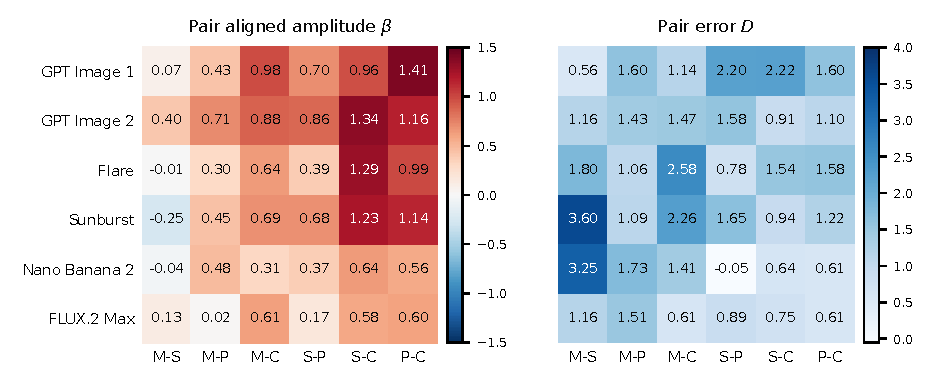
\includegraphics[width=\linewidth]{fig_pairs.pdf}
\caption{여섯 화가 쌍 각각의 정렬 진폭과 오차(M: 모네, S: 시슬레, P: 피사로, C: 세잔). 31개 특징을 모두
쓰고, 각 쌍의 참조 거리 제곱으로 정규화했다. 진폭 1은 참조와 일치하고 음수는 반대 방향을 가리키며,
오차 1은 화가를 구분하지 않는 경우에 해당한다. 반복 보정 때문에 오차가 음수가 될 수 있다.}
\label{fig:pairs}
\end{figure}

\paragraph{전체 분해.} 표~\ref{tab:decomposition-full}에 모든 성분을 실었다. 화가 미지정 기준선 대비 공통
성분은 $N_{\mathrm{free}}=G+N+I$이며, 여기서 $G$는 일반 출력과 화가 미지정 출력 사이 이동의 제곱 크기이고
$I$는 부호가 있는 교차항이다(부록~\ref{app:estimators}). 화가 미지정 기준선 대비로는 제곱 변화량의
82.5--95.7\%가 공통이다. 여기에는 유화 지시 자체가 포함되며, 두 성분을 장면 안에서 계산하면
88.6--97.2\%가 된다. 일반 기준선 대비 장면 내 공통 비율은 52.8--93.6\%이다. 표~\ref{tab:robustness}에는
표준화 단위의 제곱으로 나타낸 중심 근접도를 실었다.

\paragraph{특징군.} 표~\ref{tab:families}는 특징군별 공통 비율을 충실 기준값과 정확 차이 기준값의 평균과
함께 보여 준다. 텍스처는 색채보다 충실 기준이 높고(+2.1포인트) 정확 차이 기준은 낮으므로($-$3.2포인트;
둘 다 반올림 전 값으로 계산), 어느 기준도 텍스처와 색채의 차이를 혼자 설명하지 못한다. 31개 특징의
가중치를 바꾸면 공통 비율은 66.1--89.8\%(특징군별 동일 가중)와 65.8--86.9\%(개발 패널 공분산)가 되고,
특징을 하나씩 빼도 비율은 64.8--89.6\% 안에 머문다. 특징군의 분모가 양수가 아니었던 장면 재표집 표본은
버렸다. 그런 표본은 5,000개 가운데 공간 특징 평균에서 32개, 텍스처 평균에서 4개, 짝지은 특징군 차이에서
35개였다.

\paragraph{실제 회화 대조군.} 무작위 분할 1,000회 각각에서, 각 화가의 컬렉션(또는 화가와 내용 범주의 각
조합)에 속한 작품을 서로 겹치지 않는 두 절반으로 나눈다. 작은 쪽 절반으로 목표를 추정하고, 다른 절반에서는
의사 장면 14개(내용 범주를 쓸 때는 11개) 각각에 화가마다 서로 다른 작품 두 점을 뽑는다. 이렇게 만든 의사
장면을 각 표현에서 같은 오차 $D$로 채점한다(표~\ref{tab:genuine}). 이 대조군의 이전 판은 두 작품을 복원
추출했기 때문에 두 의사 반복이 같은 그림일 수 있었다. 한 작품과 그 자신의 곱은 화가 내 분산을 더하므로,
그 판의 평균이 부풀려졌다(첫 열의 0.234, 0.753, 0.731). 서로 다른 작품을 쓰면 의사 반복이 화가 평균의
비편향 추정이 되므로, 통합 대조군의 기댓값은 목표 자체의 잡음뿐이다. 각 컬렉션의 약 절반으로 추정한
목표라면 부록~\ref{app:estimators}의 항 $\frac34\sum_a\operatorname{tr}(\Sigma_a)/n_a$는 전체 컬렉션에서
구한 $H$의 6.7\%의 약 두 배가 되어, 관측된 0.125에 가깝다. 내용 범주별 표집은 범주 평균과 통합 평균의
차이를 더하고(0.185), 범주별 목표는 더 적은 작품에 기대어 추정된다(0.328). 생성 이미지의 오차는 전체
컬렉션을 기준으로 채점하며, 그 목표 잡음은 $H$ 보정으로 제거한 6.7\%에 해당한다(표~\ref{tab:robustness}).
따라서 이 대조군은 이 설계에서 실제 회화가 받는 점수를 기술할 뿐, 생성기가 도달할 수 있는 값의 한계를
정하지는 않는다.

\paragraph{특징의 분리 능력.} 개발 작품 221점을 표준화한 31개 특징에서 가장 가까운 참조 평균에 배정하면
매크로 정확도는 49.8\%이며, 모네 작품은 39.6\%, 시슬레 작품은 30.6\%만 맞게 분류된다. 임베딩에서는
79.8\%(CLIP)와 79.6\%(CSD)이다.

\paragraph{화가 쌍과 참조 성분.} 표~\ref{tab:coverage}를 보면, 전체 정렬 반응은 참조 산포의 66.3\%를
차지하는 첫 번째 참조 성분에 대부분 기대고 있으며, 세잔을 빼면 그 상당 부분이 사라진다. 쌍의 정렬이
강하다고 해서 쌍의 오차가 낮아지는 것은 아니다. GPT Image 1은 GPT Image 2보다 모네--시슬레 정렬이
약하지만 그 쌍의 오차는 더 낮다(그림~\ref{fig:pairs}). Flare, Sunburst, Nano Banana 2에서는 모네와
시슬레의 참조 라벨을 맞바꾸면 전체 오차가 낮아지는데, 쌍의 정렬이 음수이면 반드시 그렇게 된다.

\paragraph{장면 집계와 배율 조정.} 장면 간 변동은 Nano Banana 2가 가장 크고 FLUX.2 Max가 가장 작으며,
이 때문에 두 구성의 순서가 $D$와 $D_{\mathrm{agg}}$에서 뒤바뀐다. GPT Image 2의 차이는 제곱 크기로
참조의 약 두 배(노름으로는 1.49배)이므로, 크기의 약 0.45로 줄이면 정렬 반응보다 패턴 밖 차이가 더 많이
제거된다. 장면을 하나씩 빼고 전체 절차를 다시 적합해도, 배율 조정 후 GPT Image 2의 우위는 유지된다.

\paragraph{분포.} 표~\ref{tab:diversity}에 사전 지정된 분포 진단을 실었다. 한 화가의 이름으로 생성한
이미지 28장은 14개 장면에 걸쳐 있는데도, 총분산은 그 화가 참조 작품의 0.25--0.88배에 그친다. 에너지
거리로 보면 구성--화가 조합 24개 가운데 21개에서 이름 지정 이미지가 일반 이미지보다 그 화가의 작품에 더
가깝다. 그림~\ref{fig:projection}은 각 구성의 장면 평균한 중심화 이름 지정 평균을, $H$의 87.0\%를 담는
첫 두 참조 축 위에서 참조 차이와 나란히 보여 준다.

% 한국어판: paper/tmlr_ko/build_korean.py 가 생성한다. 직접 고치지 않는다.
% Generated by paper/tmlr/build_assets.py; do not edit by hand.
% input data/manifests/painter_specificity_v2/psv2-20260911/analysis.json sha256 c1d21b16f840a10fd253c1d558743a09671acf3d4e48601ddcc96625a5a90be0
\begin{table}[t]
\caption{사전 지정한 분포 진단(특징 31개). 대각합 비: 한 화가의 이름으로 생성한 이미지 28개(장면 14개, 반복 두 번)의 총분산을 그 화가 참조 작품의 총분산과 비교한 비. 에너지 거리: 그 이미지들과 화가의 참조 작품 사이의 거리를 화가에 걸쳐 평균한 값으로, 이름 지정 이미지와 일반 이미지 각각에 대해 계산했다. 이름 우세: 이름 지정 이미지가 더 가까운 화가의 수(네 명 중).}
\label{tab:diversity}
\vspace{2pt}
\centering\small
\begin{tabular}{@{}lrrrrrrr@{}}
\toprule
 & \multicolumn{4}{c}{대각합 비} & \multicolumn{3}{c}{에너지 거리}\\
\cmidrule(lr){2-5}\cmidrule(l){6-8}
구성 & 모네 & 시슬레 & 피사로 & 세잔 & 이름 지정 & 일반 & 이름 우세\\
\midrule
GPT Image 1 & 0.48 & 0.69 & 0.60 & 0.60 & 2.64 & 4.94 & 4\\
GPT Image 2 & 0.28 & 0.31 & 0.30 & 0.30 & 2.20 & 2.76 & 4\\
Flare & 0.27 & 0.37 & 0.32 & 0.27 & 2.11 & 2.01 & 2\\
Sunburst & 0.25 & 0.27 & 0.27 & 0.32 & 1.81 & 2.36 & 3\\
Nano Banana 2 & 0.83 & 0.71 & 0.57 & 0.88 & 2.50 & 3.43 & 4\\
FLUX.2 Max & 0.34 & 0.42 & 0.57 & 0.62 & 1.35 & 2.37 & 4\\
\bottomrule
\end{tabular}
\end{table}


\begin{figure}[ht]
\centering
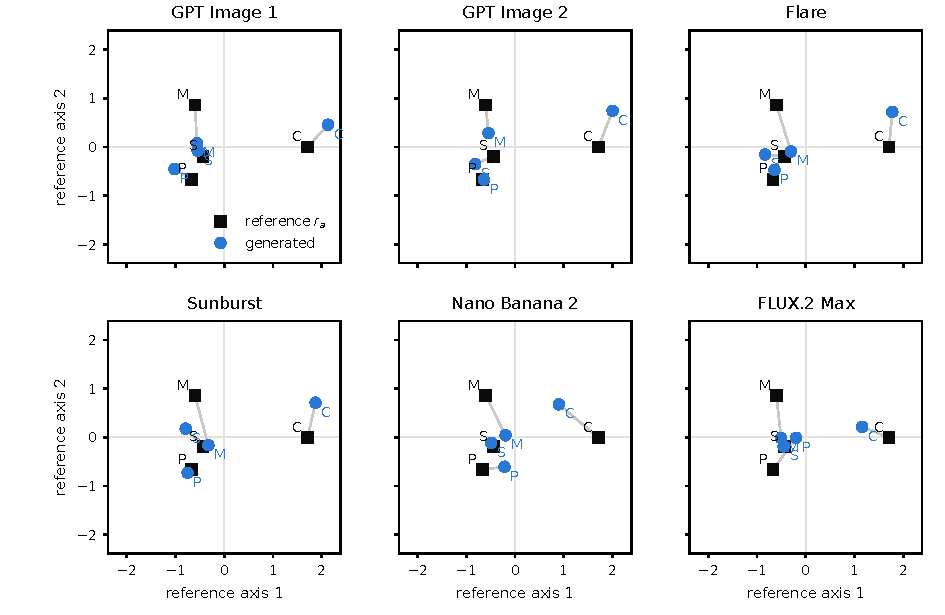
\includegraphics[width=\linewidth]{fig_projection.pdf}
\caption{31개 특징 참조 차이의 첫 두 주축 위에 나타낸 참조 차이 $r_a$(사각형)와, 각 구성에서 장면과
반복에 걸쳐 평균한 중심화 이름 지정 평균(원). M: 모네, S: 시슬레, P: 피사로, C: 세잔이며, 회색 선은 각
화가의 두 점을 잇는다. 점추정값이며, 나머지 축은 표시하지 않았다.}
\label{fig:projection}
\end{figure}

\paragraph{참조 민감도.} 내용 일치 목표는 혼합 장면이 아닌 11개 장면에 대해 제목 기반의 물, 건축, 땅
범주를 쓴다. 길 범주의 작품은 그 범주에 속하는 장면이 없으므로 통합 목표에는 들어가지만 어떤 범주
목표에도 들어가지 않는다. 출처 점검에서는 제거할 수 있는 액자, 여백, 라벨, 색 보정 띠를 기록했고, 경계가
불확실한 43곳은 그대로 두었다. 같은 복제 이미지를 시각적으로 살핀 내용 점검은 230점에서 제목 기반 범주와
달랐다. 제목 기반 라벨을 시각 라벨로 바꿔도 오차가 가장 낮은 구성은 FLUX.2 Max이다. 어떤 보정에서도 모든
작품과 특징을 유지한다.

\FloatBarrier
\section{특징군과 민감도}\label{app:sensitivity}

\paragraph{특징군.} 구성 평균으로 보면 공통 비율은 색채 특징에서 74.3\%, 공간 특징에서 71.5\%,
텍스처 특징에서 68.2\%이다. 그러나 정확 차이 기준도 텍스처에서 더 낮고(74.7\%, 색채 77.8\%, 공간
79.1\%), 모든 특징군이 각자의 기준보다 3.6--7.6포인트 아래에 있다(표~\ref{tab:families}). 따라서
텍스처--색채 차이($-$6.1포인트, [$-$13.5, $-$2.0])는 참조 차이로부터 어느 정도 예상되는 것이며,
텍스처--공간 순서는 판별되지 않는다(대응 장면 재표집의 65.2\%에서 텍스처가 더 낮다). GPT Image 1의
텍스처 비율 48.6\%는 50\%에 못 미치는 유일한 값으로, 지나치게 큰 텍스처 차이에서 비롯된다($B/H=$
3.11; 정확 차이 기준값 74.6\%). 다른 템플릿과 시드 설계로 생성한 SD-Turbo 이미지 2,000장의 이전
수집에서는 전체 특징에서 변화의 64.2\%, 텍스처에서 36.6\%가 공통이며, 전체 특징의 충실 기준값과 정확
차이 기준값은 92.5\%와 67.4\%이다(부록~\ref{app:sdturbo}). 이 수집은 같은 참조를 다시 쓰며, 회고적
점검의 역할을 한다.

\paragraph{참조 출처.} 공통 비율은 참조 컬렉션에 의존하지 않지만, 그 기준들과 일치도 점수는 참조
컬렉션에 의존한다. AI 어시스턴트가 참조 패널과 개발 패널의 복제 이미지 870장을 모두 점검하고, 그중
131장에서 액자나 색 보정 띠 같은 가장자리 요소를 잘라 냈다. 잘라 낸 결과는 사람이 확인하지 않았다.
잘라 낸 영역에 원래의 특징 척도화를 적용하면 FLUX.2 Max의 오차는 0.832가 되고, 정렬 진폭 여섯 개는
모두 양수로 남으며, 쌍별 차이 가운데 판별된 상태로 남는 것은 Flare--FLUX.2 Max뿐이다. 특징 척도화까지
다시 적합하면 FLUX.2 Max의 오차는 0.872이고, 진폭은 여전히 양수이며, Flare--FLUX.2 Max와 GPT Image
1--FLUX.2 Max가 판별된다.

\paragraph{기타 점검.} FLUX.2 Max는 장면을 하나씩 뺀 모든 경우와 정사각형 측정 창, 내용 일치 참조
목표, 두 가지 대안 특징 가중치, 두 가지 출처 보정에서 모두 31개 특징 오차 추정값이 가장 낮다
(표~\ref{tab:sensitivity}). 다만 텍스처 특징만 쓰면 Nano Banana 2가 0.886으로 FLUX.2 Max의 0.906보다
낮다(부록 표~\ref{tab:family-agreement}). 참조 화가 산포 $H$를 유한 표본 편향(6.7\%)만큼 보정하면
$\beta$, $Q$, $D-1$이 모두 같은 배수로 바뀐다. 정렬 진폭은 0.474--1.071, FLUX.2 Max의 오차는 0.787이
되고, 순서는 하나도 바뀌지 않으며, 정확 차이 비율은 59.3--85.1\%로 오른다(표~\ref{tab:robustness}).
모든 구성에서 이름 지정 이미지는 해당 화가의 참조 작품보다 덜 다양하며(대각합 비 0.25--0.88),
구성--화가 조합 24개 중 21개에서 일반 이미지보다 그 화가의 작품에 더 가깝다(표~\ref{tab:diversity}).

\FloatBarrier
\section{학습된 임베딩}\label{app:learned}

\paragraph{추출.} 공개 체크포인트
\texttt{openai/\allowbreak clip-\allowbreak vit-\allowbreak large-\allowbreak patch14}와
\texttt{tomg-\allowbreak group-\allowbreak umd/\allowbreak CSD-\allowbreak ViT-\allowbreak L}을 사용했다.
CSD는 CLIP 시각 백본에 공개된 화풍 투영을 얹은 모델이다. CSD 공개본은 논문에 보고된 벤치마크 수치와
차이가 있다고 밝히고 있으므로, 그 수치를 재현했다고 주장하지 않고 공개된 체크포인트 자체의 특성을
기술한다. 모든 이미지는 앞에서와 같이 방향과 색을 보정한 뒤, 짧은 변이 224픽셀이 되도록 바이큐빅
보간으로 크기를 조정하고, $224\times224$로 중앙을 잘라 CLIP 채널 통계로 정규화한다. 임베딩은 단위
길이로 정규화한 768차원 벡터이며, 척도 조정이나 차원 선택 없이 그 유클리드 기하와 코사인 기하를 그대로
쓴다. 고정된 시험 사례로 백엔드와 배치 크기를 바꿔 본 점검에서 결과는 좌표당 $1.3\times10^{-6}$
이내로 일치했다.

\paragraph{프로토타입 이득.} 정규화하지 않은 프로토타입 $\mu_a$(단위 참조 임베딩의 평균)를 쓰면,
$g_a^\top\mu_b$는 이미지와 참조 작품 사이의 평균 코사인 유사도이다. $g_a=\bar g+d_a$,
$\mu_a=\bar\mu+r_a$로 쓰면
\begin{equation}
\frac14\sum_a g_a^\top\mu_a-g_{\mathrm g}^\top\bar\mu
=(\bar g-g_{\mathrm g})^\top\bar\mu+\frac14\sum_a d_a^\top r_a
=(\bar g-g_{\mathrm g})^\top\bar\mu+\frac{H\widehat\beta}{4}
\end{equation}
이 성립한다. $\sum_a r_a=\sum_a d_a=0$이기 때문이다. 첫째 항은 어떤 이름이 어떤 이미지를 만들었는지에
의존할 수 없으며, 생성 이미지의 화가 라벨을 뒤섞으면 $\widehat\beta$만 바뀐다. 충실 기준값은
$g_a=\mu_a$로 두어 공통 비율 $(\bar\mu-g_{\mathrm g})^\top\bar\mu/[(\bar\mu-g_{\mathrm
g})^\top\bar\mu+H/4]$를 얻는다. $\mu_a$를 단위 프로토타입 $u_a=\mu_a/\|\mu_a\|$로 바꾸어도 점수는
이미지 임베딩에 대해 선형이므로, $\mu_a$ 대신 $u_a$를 넣은 같은 항등식이 성립한다
(표~\ref{tab:learned-settings}).

% 한국어판: paper/tmlr_ko/build_korean.py 가 생성한다. 직접 고치지 않는다.
% Generated by paper/tmlr/build_assets.py; do not edit by hand.
% input reports/painter_tmlr_diagnostics_v1/analysis.json sha256 76792fa35f90e3d8fec1a75b0eec27d69cac14ed875fce8b64096b8e2525a4d4
% input reports/painter_tmlr_diagnostics_v5/analysis.json sha256 5747902e4fae5ff111a52b5f2b8da112bc26c611555e82314b278de953981f6b
\begin{table}[t]
\caption{14개 장면을 복원 재표집할 때 각 지표에서 가장 좋은 구성(대응 재표집 5,000회; 모든 구성에 같은 장면). 백분율은 직접 작성한 장면에 대한 의존성을 나타낸다. 인식에서 생기는 동률은 먼저 나열된 구성에 귀속한다. 아래쪽 행: 정렬 비와 $D_{\mathrm{held}}$(별도의 재표집).}
\label{tab:stability}
\vspace{2pt}
\centering\small
\begin{tabular}{@{}llrlr@{}}
\toprule
지표 & 가장 자주 최고 & \% & 그다음 & \%\\
\midrule
근접도 이득, CLIP & Nano Banana 2 & 85.8 & Sunburst & 9.5\\
근접도 이득, CSD & FLUX.2 Max & 33.6 & GPT Image 1 & 26.2\\
인식, CLIP & GPT Image 2 & 98.7 & GPT Image 1 & 0.8\\
인식, CSD & GPT Image 2 & 80.4 & GPT Image 1 & 19.6\\
오차 $D$, 31개 특징 & FLUX.2 Max & 84.7 & Nano Banana 2 & 15.3\\
오차 $D$, CLIP & GPT Image 1 & 99.3 & GPT Image 2 & 0.6\\
오차 $D$, CSD & FLUX.2 Max & 47.2 & GPT Image 1 & 26.8\\
\midrule
정렬 비, 31개 특징 & GPT Image 2 & 98.0 & Nano Banana 2 & 0.7\\
정렬 비, CLIP & GPT Image 2 & 99.7 & GPT Image 1 & 0.3\\
정렬 비, CSD & GPT Image 2 & 100.0 & FLUX.2 Max & 0.0\\
$D_{\mathrm{held}}$, 31개 특징 & GPT Image 2 & 99.0 & GPT Image 1 & 0.6\\
$D_{\mathrm{held}}$, CLIP & GPT Image 2 & 99.8 & GPT Image 1 & 0.2\\
$D_{\mathrm{held}}$, CSD & GPT Image 2 & 100.0 & FLUX.2 Max & 0.0\\
\bottomrule
\end{tabular}
\end{table}

% 한국어판: paper/tmlr_ko/build_korean.py 가 생성한다. 직접 고치지 않는다.
% Generated by paper/tmlr/build_assets.py; do not edit by hand.
% input reports/painter_learned_audit_v1/analysis.json sha256 06c77de4be133afc203dda122b2816d4f866e1389999f18bc94b3d9c668f28f7
% input reports/painter_tmlr_diagnostics_v3/analysis.json sha256 2aa36a87cd6d23ee909cdf94bd9f512d5743138f1d8a8f7c236d56f33fbceb57
\begin{table}[t]
\caption{대안적 참조 설정에서 근접도 이득 가운데 공통 항이 차지하는 비율(\%). 주: 주 참조 컬렉션의 전체 복제 이미지(표~\ref{tab:learned}). 크롭: 참조 복제 이미지를 감사한 회화 영역으로 대체. 개발: 개발 패널을 참조 목표로 사용. 둘 다: 개발 패널의 감사한 영역. 단위: 인식에서처럼 단위 길이로 정규화한 주 프로토타입.}
\label{tab:learned-settings}
\vspace{2pt}
\centering\small\setlength{\tabcolsep}{3.5pt}
\begin{tabular}{@{}lrrrrrrrrrr@{}}
\toprule
 & \multicolumn{5}{c}{CLIP} & \multicolumn{5}{c}{CSD}\\
\cmidrule(lr){2-6}\cmidrule(l){7-11}
구성 & 주 & 크롭 & 개발 & 둘 다 & 단위 & 주 & 크롭 & 개발 & 둘 다 & 단위\\
\midrule
GPT Image 1 & 74.5 & 74.5 & 74.3 & 74.4 & 74.6 & 72.7 & 72.9 & 73.4 & 73.0 & 72.8\\
GPT Image 2 & 73.2 & 73.0 & 72.8 & 72.7 & 73.4 & 54.2 & 54.7 & 53.5 & 53.2 & 54.7\\
Flare & 78.8 & 78.7 & 78.9 & 79.0 & 79.0 & 65.0 & 65.5 & 65.1 & 64.9 & 65.4\\
Sunburst & 77.7 & 77.7 & 78.0 & 78.1 & 78.0 & 67.4 & 67.6 & 68.0 & 67.8 & 67.7\\
Nano Banana 2 & 83.8 & 83.9 & 83.5 & 83.7 & 83.9 & 79.7 & 79.9 & 81.3 & 81.0 & 79.6\\
FLUX.2 Max & 81.7 & 81.7 & 81.5 & 81.9 & 81.9 & 77.6 & 77.7 & 78.7 & 78.5 & 77.7\\
\bottomrule
\end{tabular}
\end{table}

% 한국어판: paper/tmlr_ko/build_korean.py 가 생성한다. 직접 고치지 않는다.
% Generated by paper/tmlr/build_assets.py; do not edit by hand.
% input reports/painter_tmlr_diagnostics_v5/analysis.json sha256 5747902e4fae5ff111a52b5f2b8da112bc26c611555e82314b278de953981f6b
\begin{table}[t]
\caption{각 표현에서 오차의 성분과 반복 의존성. $\beta$: 미보정 장면 대응 95\% 스튜던트 구간. $D$의 분해: 사전 지정한 참조 패턴 방향 부분과 패턴 외 부분(표~\ref{tab:calibration}), 그리고 패턴 외 부분의 비율. 반복 잡음: 두 반복의 중심화한 대조값 차이 제곱의 절반을 $H$에 대한 상대값으로 나타낸 것. $D=1$의 $\rho$: 두 반복이 잡음의 그만큼을 공유할 때 1보다 높은 오차가 1로 떨어지는 공통 반복 상관(부록~\ref{app:provenance}). 1보다 낮은 오차는 더 낮아질 뿐이다.}
\label{tab:embedding-calibration}
\vspace{2pt}
\centering\small\setlength{\tabcolsep}{4pt}
\begin{tabular}{@{}lcrrrrrr@{}}
\toprule
 & $\beta$ & & \multicolumn{3}{c}{$D$의 분해} & 반복 &\\
\cmidrule(lr){4-6}
구성 & 장면 & $D$ & 패턴 방향 & 패턴 외 & 패턴 외 (\%) & 잡음 $/H$ & $D=1$의 $\rho$\\
\midrule
\multicolumn{8}{@{}l}{\textit{31개 특징}}\\
GPT Image 1 & [0.806, 1.070] & 1.572 & 0.029 & 1.543 & 98.2 & 2.02 & 0.22\\
GPT Image 2 & [0.938, 1.059] & 1.226 & $-$0.003 & 1.229 & 100.2 & 0.96 & 0.19\\
Flare & [0.719, 0.824] & 1.738 & 0.054 & 1.683 & 96.9 & 0.42 & 0.64\\
Sunburst & [0.741, 0.907] & 1.641 & 0.044 & 1.598 & 97.3 & 0.58 & 0.52\\
Nano Banana 2 & [0.335, 0.549] & 1.109 & 0.317 & 0.793 & 71.5 & 2.60 & 0.04\\
FLUX.2 Max & [0.337, 0.603] & 0.801 & 0.304 & 0.497 & 62.0 & 1.67 & ---\\
\midrule
\multicolumn{8}{@{}l}{\textit{CLIP}}\\
GPT Image 1 & [0.468, 0.585] & 0.847 & 0.231 & 0.616 & 72.8 & 1.20 & ---\\
GPT Image 2 & [0.716, 0.825] & 1.061 & 0.057 & 1.004 & 94.6 & 1.13 & 0.05\\
Flare & [0.511, 0.606] & 1.057 & 0.201 & 0.856 & 81.0 & 0.80 & 0.07\\
Sunburst & [0.594, 0.709] & 1.136 & 0.129 & 1.007 & 88.6 & 0.83 & 0.14\\
Nano Banana 2 & [0.472, 0.574] & 1.078 & 0.230 & 0.848 & 78.7 & 1.59 & 0.05\\
FLUX.2 Max & [0.385, 0.490] & 1.058 & 0.316 & 0.743 & 70.2 & 1.78 & 0.03\\
\midrule
\multicolumn{8}{@{}l}{\textit{CSD}}\\
GPT Image 1 & [0.654, 0.803] & 0.735 & 0.085 & 0.650 & 88.4 & 0.73 & ---\\
GPT Image 2 & [0.889, 0.982] & 0.741 & 0.005 & 0.736 & 99.4 & 0.54 & ---\\
Flare & [0.768, 0.841] & 0.819 & 0.041 & 0.778 & 95.0 & 0.36 & ---\\
Sunburst & [0.813, 0.906] & 0.944 & 0.024 & 0.920 & 97.4 & 0.42 & ---\\
Nano Banana 2 & [0.463, 0.588] & 0.999 & 0.231 & 0.768 & 76.9 & 1.04 & ---\\
FLUX.2 Max & [0.540, 0.656] & 0.714 & 0.162 & 0.551 & 77.3 & 1.01 & ---\\
\bottomrule
\end{tabular}
\end{table}

% 한국어판: paper/tmlr_ko/build_korean.py 가 생성한다. 직접 고치지 않는다.
% Generated by paper/tmlr/build_assets.py; do not edit by hand.
% input reports/painter_tmlr_diagnostics_v1/analysis.json sha256 76792fa35f90e3d8fec1a75b0eec27d69cac14ed875fce8b64096b8e2525a4d4
\begin{table}[t]
\caption{각 임베딩에서 계산한, 이름이 더하는 제곱 변화량의 공통 비율 $N/(N+B)$ (\%)와 그 충실 모방값.}
\label{tab:learned-squared}
\vspace{2pt}
\centering\small
\begin{tabular}{@{}lrrrr@{}}
\toprule
 & \multicolumn{2}{c}{CLIP} & \multicolumn{2}{c}{CSD}\\
\cmidrule(lr){2-3}\cmidrule(l){4-5}
구성 & 관측 & 충실 & 관측 & 충실\\
\midrule
GPT Image 1 & 76.1 & 86.1 & 76.5 & 89.2\\
GPT Image 2 & 76.6 & 87.1 & 68.8 & 82.4\\
Flare & 81.7 & 88.7 & 74.6 & 86.4\\
Sunburst & 77.6 & 88.9 & 69.9 & 86.9\\
Nano Banana 2 & 82.3 & 91.2 & 77.4 & 89.7\\
FLUX.2 Max & 80.8 & 88.5 & 75.1 & 87.7\\
\bottomrule
\end{tabular}
\end{table}

% 한국어판: paper/tmlr_ko/build_korean.py 가 생성한다. 직접 고치지 않는다.
% Generated by paper/tmlr/build_assets.py; do not edit by hand.
% input reports/painter_tmlr_diagnostics_v2/analysis.json sha256 bed891f767a98f4b281b6783b1021956f4d2c3ff80becbf6b2693ee45987ef1a
\begin{table}[t]
\caption{프롬프트에 지정한 화가별로 따로 계산한 근접도 이득의 공통 부분(\%): $(\bar g-g_{\mathrm g})^\top\mu_a$를 $(g_a-g_{\mathrm g})^\top\mu_a$로 나눈 값. 100\%를 넘는 값은 그 화가의 화가 특이 항이 음수라는 뜻이다.}
\label{tab:per-painter}
\vspace{2pt}
\centering\small\setlength{\tabcolsep}{4pt}
\begin{tabular}{@{}lrrrrrrrr@{}}
\toprule
 & \multicolumn{4}{c}{CLIP} & \multicolumn{4}{c}{CSD}\\
\cmidrule(lr){2-5}\cmidrule(l){6-9}
구성 & 모네 & 시슬레 & 피사로 & 세잔 & 모네 & 시슬레 & 피사로 & 세잔\\
\midrule
GPT Image 1 & 75.4 & 85.7 & 81.2 & 59.5 & 73.8 & 79.6 & 73.1 & 62.0\\
GPT Image 2 & 78.1 & 85.5 & 91.9 & 51.6 & 68.8 & 62.1 & 64.1 & 34.6\\
Flare & 84.7 & 93.3 & 102.9 & 55.1 & 74.1 & 68.1 & 85.8 & 47.5\\
Sunburst & 90.2 & 83.7 & 93.5 & 57.2 & 75.3 & 70.4 & 78.4 & 53.4\\
Nano Banana 2 & 87.6 & 90.0 & 87.6 & 73.2 & 79.1 & 79.1 & 73.4 & 85.8\\
FLUX.2 Max & 80.5 & 105.3 & 97.0 & 57.6 & 70.6 & 86.4 & 96.9 & 64.0\\
\bottomrule
\end{tabular}
\end{table}


\paragraph{오차 성분과 반복 간 의존성.} 세 표현 모두에 대한 $D$의 분해, $\beta$의 스튜던트 $t$ 구간,
반복 잡음은 표~\ref{tab:embedding-calibration}에 있다. 임베딩에서도 패턴 밖 성분이 지배적이며, 패턴
방향 진폭이 차지하는 몫은 특징에서보다 크다.

\paragraph{잘라내기.} 생성 이미지는 정사각형이어서 인코더의 중앙 잘라내기가 이미지의 거의 전체를
보지만, 정사각형이 아닌 참조 복제 이미지는 가장자리를 잃는다. 31개 특징에서 이에 대응하는 정사각형
창 민감도 분석에서도 FLUX.2 Max의 오차가 가장 낮다(부록 표~\ref{tab:sensitivity}).

\paragraph{범위.} CSD는 CLIP 백본 위에 만들어졌고 두 인코더는 같은 이미지를 보므로, 두 인코더의 결과가
일치한다는 것은 서로 독립적인 표현 사이의 일치보다 약한 증거이다. 네 화가 모두 CSD의 화풍 태그
어휘에 들어 있으며, 두 인코더의 학습 데이터가 우리 참조와 얼마나 겹치는지는 알 수 없다. 참조 패널에
대한 점검으로, 주 프로토타입은 개발 작품 221점을 매크로 정확도 79.8\%(CLIP)와 79.6\%(CSD)로
분류한다.

\FloatBarrier
\section{홀드아웃 장면에서의 프롬프트 이름 인식}\label{app:transfer}

% 한국어판: paper/tmlr_ko/build_korean.py 가 생성한다. 직접 고치지 않는다.
% Generated by paper/tmlr/build_assets.py; do not edit by hand.
% input reports/painter_prototype_transfer_v1/analysis.json sha256 e1d1fbb924feb797f67e0907677511ed7c745335a4f2827e99d2f286e6be5448
\begin{table}[t]
\caption{홀드아웃 장면에서 프롬프트에 지정한 화가의 인식 정확도(\%; 구성당 화가 지정 이미지 112개, 우연 수준 25\%). Ref.: 가장 가까운 참조 프로토타입. Shift: 생성 이미지와 참조의 혼합 평균을 맞추는 고정된 평행이동 하나를 화가 라벨 없이 나머지 13개 장면에서 적합해 더한 뒤 같은 규칙을 적용. Gen.: 나머지 13개 장면에서 화가 라벨로 적합한 생성 이미지 프로토타입 가운데 가장 가까운 것. Shift와 Gen.은 Ref.보다, Gen.은 Shift보다 더 많은 정보를 사용한다.}
\label{tab:transfer}
\vspace{2pt}
\centering\small
\begin{tabular}{@{}lrrrrrr@{}}
\toprule
 & \multicolumn{3}{c}{CLIP} & \multicolumn{3}{c}{CSD}\\
\cmidrule(lr){2-4}\cmidrule(l){5-7}
구성 & Ref. & Shift & Gen. & Ref. & Shift & Gen.\\
\midrule
GPT Image 1 & 60.7 & 55.4 & 80.4 & 72.3 & 73.2 & 84.8\\
GPT Image 2 & 68.8 & 66.1 & 75.0 & 75.9 & 76.8 & 94.6\\
Flare & 59.8 & 59.8 & 77.7 & 62.5 & 74.1 & 92.9\\
Sunburst & 58.9 & 62.5 & 69.6 & 61.6 & 70.5 & 90.2\\
Nano Banana 2 & 51.8 & 59.8 & 63.4 & 50.9 & 61.6 & 75.0\\
FLUX.2 Max & 41.1 & 53.6 & 71.4 & 39.3 & 66.1 & 75.0\\
\midrule
Ref.\ 대비 평균 변화 (pp) & & +2.7 & +16.1 & & +10.0 & +25.0\\
\bottomrule
\end{tabular}
\end{table}


각 구성과 홀드아웃 장면 $s$에 대해, $x$를 장면 $s$에서 나온 이름 지정 이미지의 단위 임베딩,
$u_a=\mu_a/\|\mu_a\|$를 정규화한 참조 프로토타입이라 하자. 참조 규칙(표의 `참조')은 $\arg\max_a x^\top u_a$이다.
이동 규칙(표의 `이동')은 $t_{-s}=\frac14\sum_a\mu_a-\bar g_{-s}$를 계산해 $\arg\max_a(x+t_{-s})^\top u_a$로
예측한다. 여기서 $\bar g_{-s}$는 나머지 13개 장면에서 나온 이름 지정 임베딩 104개의 평균이다. 이 평행
이동은 화가 $a$의 점수에 $t_{-s}^\top u_a$를 더하는데, 이 값이 화가마다 다르기 때문에 인식 결과가 바뀔
수 있다. 모든 이름 지정 이미지에 같은 벡터를 더하므로, 중심화한 대비 $d_{sak}$와 그에 따라 $\beta$,
$Q$, $D$는 변하지 않는다. 생성 프로토타입 규칙(표의 `생성')은 화가마다 라벨이 붙은 학습 임베딩 26개의 평균을
정규화해 쓴다. 홀드아웃 장면의 반복 생성은 적합에 전혀 들어가지 않으며, 화가 미지정 이미지와 일반
이미지는 쓰지 않는다. 이 질문은 참조 규칙의 혼동 양상을 안 뒤에 정했지만, 규칙은 평행 이동 결과를
계산하기 전에 고정했다. 폴드가 서로 겹치고 장면은 직접 작성한 것이므로, 이 결과는 서술적인 폴드 외
결과이다. 참조 규칙 대비 이동 규칙의 평균 변화는 +2.7포인트(CLIP)와 +10.0포인트(CSD)이며, CSD의
FLUX.2 Max에서는 이동이 112개 판정 중 39개를 바로잡고 9개를 그르친다. 생성 프로토타입 규칙은
구성--인코더 조합 12개 모두에서 두 참조 기반 규칙보다 낫다. 즉 프롬프트에 쓴 이름은 역사적 참조를
기준으로 할 때보다 각 생성기 자신의 출력 안에서 더 잘 구분된다. 참조 출처(전체 복제 이미지 또는 점검한
회화 영역)와 참조 목표(주 컬렉션 또는 개발 패널)의 네 가지 조합에서, 평행 이동의 평균 이득은
2.2--4.0포인트(CLIP), 9.7--10.1포인트(CSD)이다.

\FloatBarrier
\section{SD-Turbo 수집}\label{app:sdturbo}

이 수집은 같은 프로젝트의 이전 미공개 거리 분석을 위해 2026년 9월 5일에 \texttt{stabilityai/sd-turbo}로
생성했으며, 해상도는 $512\times512$픽셀, 디노이징은 한 단계, 가이던스 척도는 0이다. 장면 16개, 반복
블록 25개, 다섯 조건(기준 조건과 네 이름)을 교차해 조건마다 이미지 400장을 얻었다. 각 장면과 블록
안에서 다섯 조건은 모두 같은 시드를 쓴다. 이미지 해시는 주 수집과 겹치지 않는다. 장면 설명 16개는 주
수집의 장면 설명 14개와 다른, 더 짧은 범주 수준의 문장이며(예: ``a riverbank landscape, with water
organizing the composition''), 기준 프롬프트가 이미 유화를 요청하고 이름은 ``by [painter]'' 형태로
끼워 넣는다.

블록 벡터 $v_b$, $b=1,\dots,K$ ($K=25$)에 대해, 추정량
$U(v)=[K(K-1)]^{-1}\sum_{b\ne b'}\ip{v_b}{v_{b'}}$가 두 반복 간 곱을 대신한다. 각 블록 안에서 장면을
평균하고, $\delta_{ba}$를 이름 지정 조건에서 기준 조건을 뺀 이동, $c_b$를 그 이동의 이름 평균,
$e_{ba}=\delta_{ba}-c_b$라 하자. 공통 성분은 $4U(c)$, 이름 간 성분은 $\sum_aU(e_a)$이다. 곱은 서로 다른
블록 사이에서만 만들므로, 한 블록 안에서 시드를 공유하는 다섯 조건 사이의 상관은 허용된다. 참조 평균과
척도화는 주 실험의 것을 그대로 쓴다. 보고한 범위는 블록을 한 번에 하나씩 뺀 결과로, 블록 하나에 대한
민감도를 나타낸다. 충실 기준과 정확 차이 기준은 기준 조건의 블록 평균과 같은 블록 간 곱을 쓴다.
특징군별 값은 표~\ref{tab:sdturbo}에 있다. 전체 특징에서 공통 비율은 64.2\%(블록 삭제에 따라
63.9--64.6\%)이고, 색채 특징에서 57.5\%, 공간 특징에서 84.9\%이지만 텍스처에서는 36.6\%(36.2--36.9\%)이다.
장면 안에서 계산하면 전체 72.4\%, 텍스처 48.5\%이다. 텍스처의 정확 차이 기준값은 46.5\%이다. SD-Turbo의
정렬 진폭은 0.618, 장면 평균 오차는 0.917, 장면별 오차는 1.637이고, 모네--시슬레 정렬은 0.471이다. 이
수집은 같은 참조를 다시 쓰며, 이전에 다른 방식으로 분석된 적이 있다.

% 한국어판: paper/tmlr_ko/build_korean.py 가 생성한다. 직접 고치지 않는다.
% Generated by paper/tmlr/build_assets.py; do not edit by hand.
% input reports/painter_cross_cohort_v1/analysis.json sha256 9488dfafa5779b8b065cc756804e67ad64c2841a5c62c2f9b0105f8fef13973e
% input reports/painter_tmlr_diagnostics_v2/analysis.json sha256 bed891f767a98f4b281b6783b1021956f4d2c3ff80becbf6b2693ee45987ef1a
\begin{table}[t]
\caption{SD-Turbo 수집에서 특징군별 공통 비율(\%): 장면을 통합한 값, 단일 블록 삭제 25가지에 걸친 범위, 장면 내 계산값, 그리고 충실 기준과 정확 차이 기준.}
\label{tab:sdturbo}
\vspace{2pt}
\centering\small
\begin{tabular}{@{}lrcrrr@{}}
\toprule
특징 & 공통 (\%) & 블록 삭제 & 장면 내 & 충실 & 정확 차이\\
\midrule
31개 전체 & 64.2 & 63.9--64.6 & 72.4 & 92.5 & 67.4\\
색채 (11) & 57.5 & 57.3--57.8 & 66.6 & 79.7 & 56.4\\
공간 (8) & 84.9 & 84.4--85.3 & 81.2 & 96.8 & 83.3\\
텍스처 (12) & 36.6 & 36.2--36.9 & 48.5 & 89.8 & 46.5\\
\bottomrule
\end{tabular}
\end{table}


\FloatBarrier
\section{두 번째 수집}\label{app:second}

\paragraph{프로토콜과 수정.} 네 화가 결과가 알려진 뒤, 두 번째 수집의 프로토콜은 두 추가 집단을 정하고
검정 H1과 H2(\ref{sec:inference}절) 및 집단별 분석을 고정했으며, 어떤 이미지도 생성되기 전에 요청
목록과 함께 동결되었다. 동결 기록은 승인된 시점의 프로토콜 파일과 분석 코드의 해시를 묶어 두기 때문에,
프로토콜 머리말에는 아직 ``draft''(초안)라고 적혀 있다. H2의 패널 크기 보정은 그 동결된 코드에 들어
있다. 임베딩 지표(공통 비율 구간, 인식, 근접도)에 대한 계획은 이미지를 수집하는 동안, 어떤 이미지도
측정하기 전에 고정했다. 참조 규칙은 첫 요청 전에 두 번 수정되었다. 첫째, 화가당 최소 60점이라는
프로토콜의 하한을 철회해, 그런 하한이 없던 네 화가 컬렉션과 새 컬렉션을 똑같이 다루도록 했다. 허드슨강
화파 화가 세 명과 키르히너가 이 하한에 못 미친다(표~\ref{tab:v3-panels}). 둘째, Wikimedia Commons가
이제 표준 섬네일 너비만 제공하므로, 렌더링된 파일의 너비는 1,280, 1,920, 3,840픽셀(또는 원본)이며
측정을 위해 모두 짧은 변 512픽셀로 줄였다. 제목 어휘집은 네 화가 어휘집의 용어를 모두 유지하면서, 새
화가들의 제목에 맞는 장소·풍경 용어(예: Yosemite, Catskill, piazza, wheatfield)와, 이 단어들 때문에
잘못 포함될 수 있는 인물·실내 제목을 거르는 제외 용어를 추가했다. 이 용어들은 어떤 이미지도 요청하기
전에 제목들을 보고 정했다. 관련 집단의 첫 후보였던 러시아 풍경화가 네 명은 참조를 하나도 확보하기 전에
교체했는데, 그중 세 명은 Wikidata에 기록된 유화가 너무 적었기 때문이다.

% 한국어판: paper/tmlr_ko/build_korean.py 가 생성한다. 직접 고치지 않는다.
% Generated by paper/tmlr/build_assets.py; do not edit by hand.
% input data/manifests/painter_specificity_v3/refs-20261002/determination_receipt.json sha256 39e289f1ba44c7d5fe8ae18d59d076a07eb1cefd6d105859b3565bb6576fa982
% input data/manifests/painter_specificity_v3/refs-20261002/measurement_receipt.json sha256 debf37377410a96cd64f1714a277ade667d959714c0c13bbd7af986de0795c16
\begin{table}[t]
\caption{추가한 두 화가 집단의 참조 패널: 공용(Commons) 이미지가 있는 위키데이터 회화와, 네 화가 패널과 같은 순서로 적용한 각 관문(단일 작가, 캔버스에 유화, 소장처, 공개 라이선스, 짧은 변 1,024픽셀 이상, 야외 제목) 뒤에 남은 수. 이어서 중복을 합치고 읽을 수 없는 파일을 제외한 뒤 측정한 작품 수. 분류는 제목에 따른 물/건축/길/땅이다.}
\label{tab:v3-panels}
\vspace{2pt}
\centering\footnotesize
\begin{tabular}{lrrrrrrrrr}
\toprule
화가 & 발견 & 작가 & 매체 & 소장 & 권리 & 크기 & 제목 & 측정 & W/B/R/L \\
\midrule
\multicolumn{10}{l}{\emph{세기 집단}} \\
판 라위스달 & 485 & 470 & 261 & 219 & 218 & 127 & 123 & 123 & 58/31/3/31 \\
카날레토 & 408 & 404 & 342 & 306 & 306 & 166 & 158 & 157 & 120/37/0/1 \\
반 고흐 & 887 & 887 & 818 & 638 & 638 & 587 & 255 & 255 & 25/95/12/123 \\
키르히너 & 273 & 273 & 207 & 190 & 187 & 153 & 43 & 41 & 10/17/2/14 \\
\multicolumn{10}{l}{\emph{허드슨강 화파}} \\
비어슈타트 & 481 & 481 & 228 & 138 & 138 & 103 & 92 & 92 & 36/5/0/51 \\
처치 & 153 & 152 & 101 & 81 & 81 & 51 & 47 & 47 & 11/3/0/33 \\
콜 & 172 & 172 & 108 & 99 & 99 & 63 & 36 & 36 & 7/7/0/22 \\
듀랜드 & 204 & 204 & 183 & 163 & 163 & 57 & 38 & 37 & 9/2/1/26 \\
\bottomrule
\end{tabular}
\end{table}


\paragraph{참조와 예측.} 중복 두 건을 합친 뒤 채택된 작품 790점 가운데, 지원하지 않는 형식의 파일
하나는 읽을 수 없었고, 색 프로파일이 없는 비RGB 색 공간의 파일 하나는 네 화가 컬렉션에서와 마찬가지로
측정할 수 없어서 788점이 남았다(표~\ref{tab:v3-panels}). 수집 전에 기록한 예측
(표~\ref{tab:v3-predictions})은 첫 번째 수집의 일반 출력을 사용하며, 네 화가 행은 이 논문의 값을
재현한다. 첫 번째 수집의 추출 후 삭제했던 CLIP과 CSD 체크포인트는 같은 리비전으로 다시 내려받았고,
기록된 해시와 일치했다.

% 한국어판: paper/tmlr_ko/build_korean.py 가 생성한다. 직접 고치지 않는다.
% Generated by paper/tmlr/build_assets.py; do not edit by hand.
% input data/manifests/painter_specificity_v3/refs-20261002/predictions.json sha256 65a12c297f2f2e0c2d6d7afbb313e590bf7360001cbe82c5edc5fed20040414f
\begin{table}[t]
\caption{두 번째 수집 전에 기록한 예측: 각 집단의 참조 산포 $H$와, 첫 번째 수집의 일반 출력으로 계산한 여섯 구성의 충실 기준 $N^*/(N^*+H)$. 네 화가 행은 이 논문의 값을 재현한다.}
\label{tab:v3-predictions}
\vspace{2pt}
\centering\small
\begin{tabular}{lrrrrrr}
\toprule
& \multicolumn{2}{c}{특징 31개} & \multicolumn{2}{c}{CLIP} & \multicolumn{2}{c}{CSD} \\
\cmidrule(lr){2-3}\cmidrule(lr){4-5}\cmidrule(lr){6-7}
집단 & $H$ & 충실 (\%) & $H$ & 충실 (\%) & $H$ & 충실 (\%) \\
\midrule
인상파 화가 네 명 & 5.92 & 84.8--95.2 & 0.139 & 86.1--91.2 & 0.325 & 82.4--89.7 \\
세기 집단 & 34.61 & 47.0--73.3 & 0.460 & 67.4--74.8 & 1.048 & 63.4--70.3 \\
허드슨강 화파 & 6.24 & 90.1--96.9 & 0.082 & 92.7--94.3 & 0.142 & 92.2--95.5 \\
\bottomrule
\end{tabular}
\end{table}


\paragraph{수집.} 여섯 구성은 첫 번째 수집의 경로와 요청 필드를 그대로 유지했다. 코드의 테스트는 모든
구성과 장면에서 지시문 없음 요청과 일반 요청이 첫 번째 수집의 요청과 동일한지 확인하며, 수집 당일
게이트웨이에는 모든 경로가 가격 변동 없이 올라 있었다. 요청 1,680건은 120건 단위의 장면 블록 안에서 새
시드로 순서를 무작위화했다. 듀랜드와 비어슈타트의 이름을 평범한 풍경 장면과 함께 쓴 프롬프트 두 건은
공급자의 안전 시스템이 거부했으며(HTTP 400, 요금 없음), 프로토콜에 따라 기록만 하고 다시 요청하지
않았다. 게이트웨이 시간 초과 두 건(HTTP 503)은 다시 요청해 성공했다. 새로 발생한 요금은 \$72.93이다.
수집기는 요금이 확인될 때까지 요청마다 \$5를 예약해 두고, 실패한 요청이 요금을 보고하지 않으면 그
예약을 그대로 유지한다. 그래서 두 시간 초과가 \$10을 묶어 두었고, 장부에서는 이 금액이 끝내 해제되지
않았다. 이 때문에 기록된 수정을 통해 지출 상한을 \$200에서 \$220으로 올렸으며, 이 수정은 다른 규칙을
바꾸지 않았다.

% 한국어판: paper/tmlr_ko/build_korean.py 가 생성한다. 직접 고치지 않는다.
% Generated by paper/tmlr/build_assets.py; do not edit by hand.
% input reports/painter_specificity_v3/analysis.json sha256 75ef2a23c04a5c570fd224a0ada396271ad7026ef0657a1908023daca709cbc4
\begin{table}[t]
\caption{모든 표현에서의 두 사전 지정 검정(전체 화면의 31개 특징이 주 분석이다). H1: 구성에 걸쳐 평균한, 세기 집단의 공통 비율에서 허드슨강 화파의 공통 비율을 뺀 값(퍼센트포인트)과 짝지은 장면 재표집 5,000회에서 구한 95\% 구간. H2: 화가 쌍 28개에 걸친 이름 간 거리와 참조 거리 사이의 스피어만 상관을 구성에 걸쳐 평균한 값과, 여덟 화가의 이름표 재배열 40,320가지 전부에 대한 정확 단측 $p$값. 참조 거리는 패널 크기에 대해 보정했으며, 보정하지 않은 검정을 옆에 함께 보인다. 마지막 열: 패널 크기에 대해 보정한 참조 산포.}
\label{tab:v3-tests}
\vspace{2pt}
\centering\small\setlength{\tabcolsep}{4pt}
\begin{tabular}{@{}lrcrrrrrr@{}}
\toprule
 & \multicolumn{2}{c}{H1: 세기 $-$ 허드슨} & \multicolumn{2}{c}{H2: 맨텔} & \multicolumn{2}{c}{H2, 보정 없음} & \multicolumn{2}{c}{$H$, 잡음 보정}\\
\cmidrule(lr){2-3}\cmidrule(lr){4-5}\cmidrule(lr){6-7}\cmidrule(l){8-9}
표현 & 차이 & 95\% & $\rho$ & $p$ & $\rho$ & $p$ & 세기 & 허드슨\\
\midrule
31개 특징 & $-$72.7 & [$-$76.5, $-$62.6] & 0.85 & $<$0.001 & 0.84 & $<$0.001 & 33.80 & 4.21\\
31개 특징, 중앙 정사각형 & $-$72.7 & [$-$76.5, $-$62.6] & 0.85 & 0.001 & 0.85 & 0.001 & 35.30 & 5.07\\
CLIP & $-$40.1 & [$-$41.4, $-$37.3] & 0.86 & $<$0.001 & 0.86 & $<$0.001 & 0.452 & 0.070\\
CSD & $-$47.4 & [$-$48.9, $-$44.9] & 0.92 & $<$0.001 & 0.92 & $<$0.001 & 1.034 & 0.116\\
\bottomrule
\end{tabular}
\end{table}


\paragraph{검정과 민감도.} H1과 H2는 모든 표현에서 성립하며, H2는 중앙 정사각형 창에서도, 패널 크기
보정 없이도 성립한다(표~\ref{tab:v3-tests}). 생성 이미지가 정사각형이고 공통 비율은 참조를 쓰지
않으므로, 중앙 정사각형 창에서 H1이 바뀌지 않는 것은 구성상 당연하다. 구성별 공통 비율 차이는 모든
구성에서 크다. FLUX.2 Max의 보정 구간이 넓은 것은 두 비율이 모두 재표집에서 불안정하기 때문이다. 사전
지정된 H1 코드는 분모가 양수가 아닌 재표집도 그대로 두는데, 허드슨강 화파에 대한 FLUX.2 Max에서는
5,000번의 추출 중 90번에서 $N+B\le0$이고, 비율이 $[0,1]$ 밖에 놓이는 경우는 세기 집단에서 150번,
허드슨강 화파에서 237번이다(표~\ref{tab:v3-shared}). 다른 구성에서는 분모가 양수가 아닌 경우가 없다.

\paragraph{심사 후 정의한 세부 분석.} 표~\ref{tab:v3-closeness}에서는 이 결과에 대한 첫 심사 후에
작성한 계획에 따라 두 검정을 서술적으로 나누어 본다. 점추정값은 심사자들이 이미 계산해 두었으며, 구간은
새로 계산한 것이다. H2는 세기 집단 안과 집단 사이에서 성립하지만, 참조 차이가 작고 쌍이 여섯 개뿐인
허드슨강 화파 안에서는 약하다. 충실한 모방자라면 특징에서 세기 집단과 허드슨강 화파의 차이가
30.9포인트일 것이므로, 나머지 41.8포인트는 생성기가 이름을 얼마나 강하게 구분하는지에서 나온다.
표~\ref{tab:v3-readouts}에는 본문에서 인용하지 않은 임베딩 계획의 지표를 더했다.

% 한국어판: paper/tmlr_ko/build_korean.py 가 생성한다. 직접 고치지 않는다.
% Generated by paper/tmlr/build_assets.py; do not edit by hand.
% input reports/painter_specificity_v3/analysis.json sha256 75ef2a23c04a5c570fd224a0ada396271ad7026ef0657a1908023daca709cbc4
\begin{table}[t]
\caption{각 집단의 참조 차이와 이름 간 차이의 일치(31개 특징, 두 번째 수집). 표~\ref{tab:agreement}에서처럼, 보정하지 않은 짝지은 장면 스튜던트 구간과 함께 정렬 진폭 $\beta$와 오차 $D$, 상대 크기 $Q$, 정렬 비, 보류 재척도 오차, 그리고 중심점 근접도 이득(식~\ref{eq:prototype-gain}, 여기서는 특징에서)에서 공통 항이 차지하는 비율.}
\label{tab:v3-detail}
\vspace{2pt}
\centering\small\setlength{\tabcolsep}{4pt}
\begin{tabular}{@{}lrcrrrcrr@{}}
\toprule
구성 & $\beta$ & 95\% & $Q$ & $\beta/\sqrt{Q}$ & $D$ & 95\% & $D_{\mathrm{held}}$ & 공통 이득 (\%)\\
\midrule
\multicolumn{9}{l}{\emph{세기 집단}}\\
GPT Image 1 & 1.28 & [1.11, 1.45] & 3.13 & 0.72 & 1.58 & [0.74, 2.41] & 0.50 & 100.7\\
GPT Image 2 & 1.14 & [1.06, 1.22] & 2.22 & 0.76 & 0.94 & [0.75, 1.13] & 0.42 & 73.0\\
Flare & 1.29 & [1.21, 1.38] & 2.58 & 0.80 & 0.99 & [0.76, 1.23] & 0.35 & 76.2\\
Sunburst & 1.24 & [1.19, 1.30] & 2.61 & 0.77 & 1.12 & [0.84, 1.40] & 0.41 & 89.1\\
Nano Banana 2 & 1.04 & [0.93, 1.15] & 2.21 & 0.70 & 1.13 & [0.50, 1.77] & 0.53 & 86.2\\
FLUX.2 Max & 0.84 & [0.75, 0.93] & 1.41 & 0.71 & 0.73 & [0.60, 0.85] & 0.50 & 31.5\\
\multicolumn{9}{l}{\emph{허드슨강 화파}}\\
GPT Image 1 & $-$0.01 & [$-$0.12, 0.09] & 0.22 & $-$0.03 & 1.25 & [0.86, 1.64] & 1.00 & --\\
GPT Image 2 & 0.04 & [$-$0.06, 0.15] & 0.12 & 0.13 & 1.03 & [0.75, 1.31] & 1.05 & 100.2\\
Flare & $-$0.01 & [$-$0.09, 0.06] & 0.61 & $-$0.01 & 1.63 & [1.32, 1.95] & 1.00 & 103.3\\
Sunburst & 0.11 & [0.01, 0.22] & 0.48 & 0.16 & 1.26 & [1.04, 1.47] & 0.98 & 101.4\\
Nano Banana 2 & 0.20 & [$-$0.01, 0.40] & 0.65 & 0.24 & 1.26 & [0.27, 2.25] & 1.14 & 99.7\\
FLUX.2 Max & 0.12 & [$-$0.01, 0.25] & 0.22 & 0.26 & 0.98 & [0.69, 1.26] & 1.14 & 86.7\\
\bottomrule
\end{tabular}
\end{table}

% 한국어판: paper/tmlr_ko/build_korean.py 가 생성한다. 직접 고치지 않는다.
% Generated by paper/tmlr/build_assets.py; do not edit by hand.
% input reports/painter_specificity_v3/analysis.json sha256 75ef2a23c04a5c570fd224a0ada396271ad7026ef0657a1908023daca709cbc4
% input reports/painter_tmlr_diagnostics_v6/analysis.json sha256 16b91e3b0151ab29ef142cdea4a5951a2df40e87d4058ff255eeb20094f4f4af
\begin{table}[t]
\caption{임베딩에서 본 추가한 두 집단: 장면 재표집 5,000회에서 구한 95\% 구간을 붙인 공통 비율과 충실한 모방자 벤치마크, 정렬 진폭, 정렬 비, 오차, 근접도 이득에서 공통 항이 차지하는 비율(식~\ref{eq:prototype-gain}), 네 화가 중 선택 인식(매크로 정확도, 우연 수준 25\%).}
\label{tab:v3-embeddings}
\vspace{2pt}
\centering\footnotesize\setlength{\tabcolsep}{3.5pt}
\begin{tabular}{@{}lrcrrrrrr@{}}
\toprule
구성 & 공통 (\%) & 95\% & 충실 (\%) & $\beta$ & $\beta/\sqrt{Q}$ & $D$ & 공통 이득 (\%) & 인식 (\%)\\
\midrule
\multicolumn{9}{l}{\emph{CLIP, 세기 집단}}\\
GPT Image 1 & 47.0 & [44.7, 50.4] & 64.6 & 0.58 & 0.57 & 0.86 & 29.5 & 71.9\\
GPT Image 2 & 47.9 & [46.5, 51.9] & 68.6 & 0.69 & 0.61 & 0.89 & 45.5 & 85.4\\
Flare & 51.8 & [50.0, 55.3] & 71.1 & 0.57 & 0.53 & 1.04 & 48.7 & 83.3\\
Sunburst & 52.0 & [50.0, 55.3] & 71.6 & 0.67 & 0.58 & 0.98 & 46.2 & 85.4\\
Nano Banana 2 & 60.7 & [57.3, 64.6] & 74.3 & 0.62 & 0.59 & 0.86 & 49.0 & 81.2\\
FLUX.2 Max & 53.9 & [51.2, 57.6] & 70.9 & 0.63 & 0.59 & 0.89 & 46.2 & 76.0\\
\multicolumn{9}{l}{\emph{CLIP, 허드슨강 화파}}\\
GPT Image 1 & 97.5 & [95.1, 99.6] & 92.1 & 0.14 & 0.25 & 1.02 & 96.2 & 35.4\\
GPT Image 2 & 98.1 & [96.7, 99.0] & 92.3 & 0.10 & 0.21 & 1.01 & 98.2 & 29.2\\
Flare & 89.7 & [85.3, 93.4] & 93.2 & 0.25 & 0.26 & 1.44 & 95.0 & 38.5\\
Sunburst & 88.6 & [83.5, 92.7] & 93.6 & 0.31 & 0.29 & 1.51 & 94.5 & 43.8\\
Nano Banana 2 & 87.4 & [84.0, 90.9] & 94.1 & 0.39 & 0.39 & 1.24 & 92.5 & 50.0\\
FLUX.2 Max & 93.0 & [87.0, 96.3] & 92.8 & 0.18 & 0.24 & 1.19 & 95.7 & 35.4\\
\multicolumn{9}{l}{\emph{CSD, 세기 집단}}\\
GPT Image 1 & 46.2 & [44.8, 48.2] & 66.2 & 0.75 & 0.67 & 0.74 & 6.5 & 76.0\\
GPT Image 2 & 40.6 & [39.8, 42.7] & 62.8 & 0.95 & 0.76 & 0.67 & 15.4 & 89.6\\
Flare & 44.3 & [43.2, 46.5] & 69.2 & 0.83 & 0.69 & 0.77 & 23.4 & 83.3\\
Sunburst & 44.2 & [43.0, 46.6] & 68.6 & 0.93 & 0.74 & 0.72 & 25.9 & 85.4\\
Nano Banana 2 & 55.4 & [52.1, 58.6] & 70.6 & 0.74 & 0.68 & 0.71 & 40.7 & 76.0\\
FLUX.2 Max & 51.7 & [48.9, 54.9] & 63.6 & 0.75 & 0.71 & 0.61 & 32.6 & 72.9\\
\multicolumn{9}{l}{\emph{CSD, 허드슨강 화파}}\\
GPT Image 1 & 97.3 & [96.1, 98.2] & 93.2 & 0.12 & 0.21 & 1.08 & 95.1 & 31.2\\
GPT Image 2 & 98.3 & [97.2, 99.0] & 93.6 & 0.11 & 0.23 & 1.02 & 98.3 & 32.3\\
Flare & 93.2 & [91.8, 94.4] & 95.3 & 0.19 & 0.21 & 1.45 & 96.5 & 34.4\\
Sunburst & 92.3 & [90.4, 93.9] & 95.4 & 0.30 & 0.31 & 1.37 & 95.4 & 45.8\\
Nano Banana 2 & 92.3 & [89.4, 94.6] & 95.4 & 0.38 & 0.40 & 1.15 & 94.3 & 44.8\\
FLUX.2 Max & 93.2 & [88.5, 96.7] & 92.1 & 0.20 & 0.35 & 0.94 & 94.9 & 38.5\\
\bottomrule
\end{tabular}
\end{table}

% 한국어판: paper/tmlr_ko/build_korean.py 가 생성한다. 직접 고치지 않는다.
% Generated by paper/tmlr/build_assets.py; do not edit by hand.
% input reports/painter_tmlr_diagnostics_v7/analysis.json sha256 385f089c29f6853d79c9560dd80243b6ac331583334f03801e4e11b6722aac74
\begin{table}[t]
\caption{심사 후에 정의한 사전 지정 검정의 두 가지 분해(서술적). 왼쪽: 구성에 걸쳐 평균한 H2 스피어만 상관을 28쌍 전체, 각 집단 안의 6쌍, 두 집단 사이의 16쌍에 대해 계산했다. 오른쪽: H1의 세기 집단 대 허드슨강 화파 평균 차이를 관측값과 충실한 모방자(가까움만 반영)에 대해 제시하고, 관측 차이에서 충실 차이를 뺀 초과분을 함께 제시한다. 구간은 대응 장면 재표집 5,000회로 얻은 95\% 구간이다.}
\label{tab:v3-closeness}
\vspace{2pt}
\centering\footnotesize\setlength{\tabcolsep}{3.5pt}
\begin{tabular}{@{}lrrrrrrcrc@{}}
\toprule
 & \multicolumn{4}{c}{쌍 유형별 H2 (스피어만)} & \multicolumn{5}{c}{세기 $-$ 허드슨 공통 비율 (포인트)}\\
\cmidrule(lr){2-5}\cmidrule(l){6-10}
표현 & 전체 & 세기 & 허드슨 & 집단 간 & 관측 & 충실 & 95\% & 초과분 & 95\%\\
\midrule
특징 31개 & 0.85 & 0.78 & 0.09 & 0.74 & $-$72.7 & $-$30.9 & [$-$32.9, $-$26.6] & $-$41.8 & [$-$47.2, $-$34.9]\\
CLIP & 0.86 & 0.73 & 0.49 & 0.76 & $-$40.1 & $-$22.9 & [$-$23.5, $-$20.4] & $-$17.3 & [$-$19.2, $-$15.7]\\
CSD & 0.92 & 0.88 & 0.27 & 0.85 & $-$47.4 & $-$27.3 & [$-$28.5, $-$25.0] & $-$20.0 & [$-$21.7, $-$18.7]\\
\bottomrule
\end{tabular}
\end{table}

% 한국어판: paper/tmlr_ko/build_korean.py 가 생성한다. 직접 고치지 않는다.
% Generated by paper/tmlr/build_assets.py; do not edit by hand.
% input reports/painter_specificity_v3/analysis.json sha256 75ef2a23c04a5c570fd224a0ada396271ad7026ef0657a1908023daca709cbc4
% input reports/painter_tmlr_diagnostics_v6/analysis.json sha256 16b91e3b0151ab29ef142cdea4a5951a2df40e87d4058ff255eeb20094f4f4af
\begin{table}[t]
\caption{두 번째 수집의 추가 임베딩 지표로, 이미지를 측정하기 전에 정했다. 위: 여덟 화가 전체 중 인식(매크로 정확도, \%, 우연 수준 12.5\%). 아래, 여섯 구성에 걸쳐: 정렬 비와 네 화가 중 인식 사이의 스피어만 상관, 그리고 근접도 이득과 그 두 항 사이의 피어슨 상관(식~\ref{eq:prototype-gain}).}
\label{tab:v3-readouts}
\vspace{2pt}
\centering\small
\begin{tabular}{@{}lrrrr@{}}
\toprule
 & \multicolumn{2}{c}{CLIP} & \multicolumn{2}{c}{CSD}\\
\cmidrule(lr){2-3}\cmidrule(l){4-5}
 & 세기 & 허드슨 & 세기 & 허드슨\\
\midrule
GPT Image 1 & 65.6 & 34.4 & 64.6 & 31.2\\
GPT Image 2 & 78.1 & 29.2 & 87.5 & 32.3\\
Flare & 62.5 & 38.5 & 76.0 & 34.4\\
Sunburst & 69.8 & 43.8 & 83.3 & 45.8\\
Nano Banana 2 & 74.0 & 50.0 & 75.0 & 44.8\\
FLUX.2 Max & 68.8 & 35.4 & 69.8 & 38.5\\
\midrule
스피어만: 정렬 비와 네 화가 중 인식 & 0.29 & 0.94 & 0.64 & 0.66\\
이득과 공통 항의 상관 & 0.97 & 0.99 & 0.83 & 1.00\\
이득과 화가 특이 항의 상관 & 0.75 & 0.54 & 0.34 & 0.54\\
\bottomrule
\end{tabular}
\end{table}


\paragraph{두 수집 사이의 변화.} 두 수집의 지시문 없음 요청과 일반 요청은 동일하다. 반복 잡음 없이
추정한 두 수집의 장면 평균 사이 제곱 거리는, 첫 번째 수집의 반복 잡음에 대한 상대값으로 31개 특징에서
구성과 조건에 걸쳐 $-$0.61에서 0.48까지, 임베딩에서 $-$0.29에서 0.24까지이다(표~\ref{tab:v3-drift}).
영에 가까운 값은 두 반복 사이의 잡음을 넘어서는 변화가 없음을 뜻한다.

% 한국어판: paper/tmlr_ko/build_korean.py 가 생성한다. 직접 고치지 않는다.
% Generated by paper/tmlr/build_assets.py; do not edit by hand.
% input reports/painter_specificity_v3/analysis.json sha256 75ef2a23c04a5c570fd224a0ada396271ad7026ef0657a1908023daca709cbc4
\begin{table}[t]
\caption{동일한 요청에 대한 두 수집 사이의 변화: 지시문 없음 조건과 일반 조건에서 첫 번째 수집과 두 번째 수집의 장면 평균 사이 제곱 거리를 반복 잡음 없이 추정해 첫 번째 수집의 반복 잡음으로 나눈 값(0은 변화 없음, 1 근처나 그 이상은 두 반복이 서로 다른 만큼 큰 변화).}
\label{tab:v3-drift}
\vspace{2pt}
\centering\small
\begin{tabular}{@{}lrrrrrr@{}}
\toprule
 & \multicolumn{2}{c}{특징 31개} & \multicolumn{2}{c}{CLIP} & \multicolumn{2}{c}{CSD}\\
\cmidrule(lr){2-3}\cmidrule(lr){4-5}\cmidrule(l){6-7}
구성 & 없음 & 일반 & 없음 & 일반 & 없음 & 일반\\
\midrule
GPT Image 1 & $-$0.15 & 0.22 & $-$0.25 & 0.04 & $-$0.29 & 0.18\\
GPT Image 2 & 0.17 & 0.24 & 0.22 & 0.03 & 0.22 & $-$0.00\\
Flare & $-$0.15 & 0.15 & 0.03 & 0.07 & $-$0.15 & 0.01\\
Sunburst & 0.48 & $-$0.13 & $-$0.05 & $-$0.09 & 0.03 & $-$0.03\\
Nano Banana 2 & $-$0.27 & $-$0.14 & $-$0.06 & $-$0.18 & $-$0.14 & $-$0.14\\
FLUX.2 Max & $-$0.10 & $-$0.61 & 0.14 & 0.24 & $-$0.09 & 0.16\\
\bottomrule
\end{tabular}
\end{table}


\FloatBarrier
\section{증거와 재현}\label{app:replay}

이 논문의 모든 분석은 보관된 특징 벡터나 임베딩을 읽고, 입력을 SHA-256으로 기록한 버전별 결과 파일을
쓴다. 모든 표와 그림~\ref{fig:benchmark}, \ref{fig:v3-pairs}, \ref{fig:pairs}, \ref{fig:projection}은
이 결과 파일에서 생성되며, 그림~\ref{fig:schematic}도 같은 스크립트가 만든다. 그림~\ref{fig:examples}만은
정적 이미지 패널이며, 그 바이트와 선정 목록을 해시로 확인한다. 점검 스크립트는 입력 해시를 검증하고,
생성되는 모든 표와 그림을 바이트 단위까지 똑같이 다시 만들며, 본문에 인용된 등록 수치마다 다시 계산한
값과 같은지, 그리고 그 수치에 대해 기록된 문장에 실제로 나오는지 확인한다. 이 점검은 보고된 수치가
보관된 측정값에서 나온다는 것을 보장할 뿐, 픽셀에서 특징을 다시 추출하지는 않는다.


\end{document}
